\documentclass[10pt,twoside,lineno]{article}
% Use the lineno option to display guide line numbers if required.

% pdftk grammar_optim_paper.pdf pnas-word-order-si.pdf cat output submission.pdf


%\usepackage{lineno}
%\linenumbers

%\templatetype{pnassupportinginfo}

% \readytosubmit %% Uncomment this line before submitting, so that the instruction page is removed.

\usepackage{amsmath}
\usepackage{tikz-dependency}
\DeclareMathOperator*{\argmax}{arg\,max}
\DeclareMathOperator*{\argmin}{arg\,min}
\DeclareMathOperator{\E}{\mathop{\mathbb{E}}}



\usepackage{footnote}
\makesavenoteenv{tabular}
\makesavenoteenv{table}

\usepackage{siunitx}

\usepackage[cm]{fullpage}

\usepackage{longtable}


\usepackage[numbers]{natbib}

\usepackage{hyperref}

\usepackage{amssymb}% http://ctan.org/pkg/amssymb
\usepackage{pifont}% http://ctan.org/pkg/pifont
\newcommand{\cmark}{\ding{51}}%
\newcommand{\xmark}{\ding{55}}%

\usepackage[english]{babel}
\usepackage[utf8]{inputenc}
\usepackage{bm}
\usepackage{graphicx}
\usepackage{tikz}
\usepackage{xcolor}
\usepackage{url}
\usepackage{rotating}
\usepackage{multirow}
\usepackage{natbib}
\usepackage{arydshln}

\newcommand{\key}[1]{\textbf{#1}}



\renewcommand{\thefigure}{S\arabic{figure}}
\renewcommand{\thetable}{S\arabic{table}}
\renewcommand{\thesection}{S\arabic{section}}

\newcommand{\utterance}{\mathcal{U}}
\newcommand{\tree}{\mathcal{T}}



\usepackage{mathtools}
\DeclarePairedDelimiter{\ceiling}{\lceil}{\rceil}

\title{Supplemental Materials for ``Universals of word order result from optimization of grammars for efficient communication''}
\author{
        Michael Hahn \\
                Department of Linguistics\\
       Stanford University
            \and
       Daniel Jurafsky\\
       Department of Linguistics\\
       Stanford University \\
       \and
       Richard Futrell\\
       Department of Language Science\\
       University of California, Irvine
}
%\author{
%Michael Hahn, Daniel Jurafsky, Richard Futrell}

%\correspondingauthor{Michael Hahn.\\E-mail: mhahn2@stanford.edu}

\begin{document}
\maketitle




\tableofcontents


\section{Formalization of Greenberg Correlation Universals}\label{sec:correlations}


Here we describe how we selected the word order correlations in Table 1 of the main paper, and how we formalized these using syntactic relations defined by Universal Dependencies.

We base our formalization on the comprehensive study by Dryer \cite{dryer1992greenbergian}.\footnote{Regarding the objections by \citet{dunn2011evolved}, we refer to the follow-ups by \citet{levy2011computational}, and \citet{croft2011greenbergian}.}
Greenberg's original study was based on 30 languages; more recently, Dryer \cite{dryer1992greenbergian} documented the word order correlations based on typological data from 625 languages.
\citet{dryer1992greenbergian} formulated these universals as correlations between the order of objects and verbs and the orders of other syntactic relations.
We test our ordering grammars for these correlations by testing whether the coefficients for these syntactic relations have the same sign as the coefficient of the verb-object relation.
Testing correlations is therefore constrained by the degree to which these relations are annotated in UD.
The verb--object relation corresponds to the  \emph{obj} relation defined by UD.
While most of the other relations also correspond to UD relations, some are not annotated reliably.
We were able formalize eleven out of Dryer's sixteen correlations in UD.
Six of these could not be expressed individually in UD, and were collapsed into three coarse-grained correlations:
First, tense/aspect and negative auxiliaries are together represented by the \emph{aux} relation in UD.
Second, the relation between complementizers and adverbial subordinators with their complement clauses is represented by the \emph{mark} relation.
Third, both the verb-PP relation and the relation between adjectives and their standard of comparison is captured by the \emph{obl} relation.

The resulting operationalization is shown in Table~\ref{table:greenberg-dryer}.
For each relation, we show the direction of the UD syntactic relation: $\rightarrow$ indicates that the verb patterner is the head; $\leftarrow$ indicates that the object patterner is the head.

As described in \emph{Materials and Methods}, we follow \citet{futrell2015largescale} in converting the Universal Dependencies format to a format closer to standard syntactic theory, promoting adpositions, copulas, and complementizers to heads.
As a consequence, the direction of the relations \emph{case}, \emph{cop}, and \emph{mark} is reversed compared to Universal Dependencies.
For clarity, we refer to these reversed relations as \emph{lifted\_case}, \emph{lifted\_cop}, and \emph{lifted\_mark}.



\begin{table*}[ht]
	\begin{center}
\small{
\begin{tabular}{|l|ll|l|l|}
	\hline
&	\multicolumn{2}{c|}{Correlates with...}   &          \multirow{2}{*}{UD Relation}   & \multirow{2}{*}{\citet{greenberg1963universals}}    \\ 
&	verb & object & &   \\ \hline \hline % \textsc{verb} $\xrightarrow{obj}$ \textsc{noun}
%adp. &
\raisebox{.5pt}{\textcircled{\raisebox{-.9pt} {1}}}&adposition    &    NP    &  $\xrightarrow{lifted\_case}$   & 3, 4   \\ \hline
\raisebox{.5pt}{\textcircled{\raisebox{-.9pt} {2}}}&copula  verb  &    predicate    &    $\xrightarrow{lifted\_cop}$   & --    \\\hline
\multirow{2}{*}{\raisebox{.5pt}{\textcircled{\raisebox{-.9pt} {3}}}}&tense/aspect auxiliary    &    VP    &    \multirow{2}{*}{$\xleftarrow{aux}$}   & 16, 13  \\
&	negative auxiliary    &    VP    &    & -- \\ \hline
\raisebox{.5pt}{\textcircled{\raisebox{-.9pt} {4}}}&noun    &    genitive    &   $\xrightarrow{nmod}$ & 2, 23   \\ \hline
\raisebox{.5pt}{\textcircled{\raisebox{-.9pt} {5}}}&noun    &    relative clause    &    $\xrightarrow{acl}$ &  24    \\ \hline
\multirow{2}{*}{\raisebox{.5pt}{\textcircled{\raisebox{-.9pt} {6}}}}&complementizer    &    S    &   \multirow{2}{*}{$\xrightarrow{lifted\_mark}$}  & --    \\
&	adverbial subordinator & S &  & -- \\ \hline
\multirow{2}{*}{\raisebox{.5pt}{\textcircled{\raisebox{-.9pt} {7}}}}&	adjective & std. of comp. & \multirow{2}{*}{$\xrightarrow{obl}$} & --\\
&verb    &    PP    &    & 22   \\\hline
\raisebox{.5pt}{\textcircled{\raisebox{-.9pt} {8}}}&`want'    &    VP    &    $\xrightarrow{xcomp}$   & 15   \\\hline
\end{tabular}
}
	\end{center}
	\caption{Greenbergian Correlations based on Dryer \cite{dryer1992greenbergian}, with operationalizations with Universal Dependencies using the modified format of \cite{futrell2015largescale} (see text).
	For reference, we also provide the numbers of the closest corresponding universals stated in Greenberg's original study, to the extent that this is possible.
	}\label{table:greenberg-dryer}
\end{table*}



\paragraph{Excluded Correlations}
Here, we discuss in more detail the five correlations from Dryer's study that we had to exclude.
First, we excluded three correlations that are not annotated reliably in UD, and are only relevant to some of the world's languages: Question particles, plural words (i.e., independent plural markers), and articles.
All three types of elements occur at most in parts of the 51 UD languages, and none of them is annotated reliably in those languages where they occur.
Among these three types of elements, the one most prominent in our sample of 51 languages is articles, which occur in many European languages.
However, UD subsumes them under the \emph{det} relation, which is also used for other highly frequent elements, such as demonstratives and quantifiers.
%Testing this correlation would require augmenting these corpora with detailed annotation of articles, which is beyond the scope of this study.
The other elements (question particles and plural words) are found at most in a handful of UD languages, and are not specifically annotated in these either.

We also excluded the verb-manner adverb correlation.
UD does not distinguish manner adverbs from other elements labeled as adverbs, such as sentence-level adverbs and negation markers, whose ordering is very different from manner adverbs.
All types of adverbs are unified under the \emph{advmod} relation.
In the real orderings in our sample of 51 UD languages, the dominant ordering of \emph{advmod} almost always matches that of subjects -- that is, \emph{advmod} dependents are predominantly ordered after the verb only in VSO languages.
This observed ordering behavior in the 51 languages is very different from that documented for manner adverbs by Dryer, showing that a large part of \emph{advmod} dependencies as annotated in UD consists of elements that are not manner adverbs.



We further excluded the verb-subject correlation, which is not satisfied by much more than half of the world's languages (51 \% among those with annotation in the \emph{World Atlas of Language Structures} \cite{wals-81}, with clear violation in 35.4 \%).
It is satisfied only in 33\% of our sample of 51 UD languages, as quantified using the grammars we extracted.
Dryer \cite{dryer1992greenbergian} counts this as a correlation since he describes the distribution of subject order as an interaction between a weak correlation with object order, and a very strong dominance principle favoring SV orderings.
We focus on the modeling of correlations, and leave dominance principles to future research.
We therefore excluded this correlation here.
%We note that efficiency makes predictions compatible with the pattern observed in our sample of 51 languages, potentially in line with the noisy-channel explanation of SVO described by~\cite{gibson2013noisy} (see Table~\ref{tab:all-predictions}).



%croft2011greenbergian
%dryer2011evidence


\paragraph{Other Greenberg Universals}
Greenberg~\cite{greenberg1963universals} stated a total of 45 universals.
Twenty of these concern the structure of individual words (as opposed to word order, which we focus on here), and many of those have been argued to be explained by the ``dual pressures'' idea \cite{haspelmath2006against}.
The other 25 universals concern word order; Dryer \cite{dryer1992greenbergian} reformulated most of these as correlations with verb-object order; these form the basis of our formalization in Table~\ref{table:greenberg-dryer}. %, finding 16 correlations to likely be universal.
%Excluding universals not annotated in available databases, and merging some that can only be tested together we arrived at the eight correlations shown in Table~\ref{table:greenberg-dryer}.
%Testing efficiency on the excluded correlations would be feasible with additional annotation of data.
%For instance, one of these could be tested by labeling the existing databases for the distinction between manner adverbs from other kinds of adverbs.
%For another one, it would be necessary to annotate databases for additional languages that have independent plural markers (e.g., Hawaiian).
There are a few other well-supported word order universals that are not correlations with verb-object order.
This includes dominance principles~\cite{croft2003typology} such as the strong preference for subjects to precede objects.
Furthermore, there has been interest in Greenberg's universals 18 and 20, which describe correlations not with verb-object order, but of different elements of noun phrases~\cite{cinque2005deriving, culbertson2014language, dryer2018order}.
Future work should examine whether these universals can also be linked to efficiency optimization.


\paragraph{Evaluating Accuracy of Formalization}
An anonymous reviewer notes that the mapping between Dryer's relations and UD is not perfect, since some of the UD relations subsume other relations.
Here we show that this is not a problem, since the ordering of the various relations subsumed under the UD label strongly agree typologically.

\begin{enumerate}
	\item Correlation \raisebox{.5pt}{\textcircled{\raisebox{-.9pt} {3}}} captures correlations with inflected tense, aspect, and negation auxiliaries as stated by \citet{dryer1992greenbergian}; however, \emph{aux} aso encompasses other types of auxiliaires, such as modals.
We note that other authors, including \citet{greenberg1963universals}, have stated the correlation for all inflected auxiliaries; for further references, we refer to \citet[Number 501]{plank2000universals}.

We used the UD treebanks to confirm that different auxiliaries tend to pattern together, and that the most frequent order of the \emph{aux} relation coincides with that of inflected tense-aspect or negation auxiliaries.

We collected, for each UD language, all dependents of the \emph{aux} dependency, occurring at least 10 times, and compared their dominant orders, which we operationalized as their more common order in the treebank (auxiliary--head or head--auxiliary).
The dependency occurs in all but two very small treebanks (Telugu and Irish).
In 43 languages, all extracted auxiliaries had the same dominant order, with the possible exception of uninflected particles labeled \emph{aux} (Croatian, German, Polish, Ukrainian).
In three languages (Ancient Greek, Russian), there were other auxiliaries with different dominant order, but these were modal or passive auxiliaries.
Finally, in three languages (Afrikaans, Old Church Slavonic, and Persian), not all tense-aspect auxiliaries showed the same dominant order as the \emph{aux} dependency overall.
For instance, in Persian, the perfect auxiliary \emph{budan} follows the main verb, whereas the future auxiliary \emph{xaastan xaah-} precedes it~\citep[pp. 117, 121]{mace2015persian}.
%		(1) In Afrikaans, the past auxiliary \emph{het} shows dominant aux-head order, whereas the overall most common order of auxiliaries is head-aux (e.g. future auxiliary \emph{sal}).
%		Finally, in Old Church Slavonic, most aux dependencies have the reflexive \emph{sebe} which tends to precede the head, whereas inflected verbal auxiliaries (primarily, forms of \emph{byti}) have opposite order, leading to a seeming violation of the correlation  \raisebox{.5pt}{\textcircled{\raisebox{-.9pt} {3}}}.


Taken together, this shows that the dominant order of the \emph{aux} relation strongly coincides with that of inflected tense-aspect auxiliaries, except for a small number of languages where different tense-aspect auxiliaries show different orders.



\item Correlation \raisebox{.5pt}{\textcircled{\raisebox{-.9pt} {4}}} is formalized using \emph{nmod} which covers not only genitives, but also all other noun-modifying NPs and PPs.
	The evaluation of extracted grammars against WALS (Table~\ref{tab:grammars-wals}) shows that, among the 37 languages where WALS has an entry, the dominant direction of \emph{nmod} agrees with that of genitives, with two exceptions (Danish and Swedish).

TODO figure out why

\item Correlation \raisebox{.5pt}{\textcircled{\raisebox{-.9pt} {5}}} is formalized using \emph{acl}, which covers not just relative clauses, but also other adnominal clauses.
	In the WALS evaluation (Table~\ref{tab:grammars-wals}), the dominant order of \emph{acl} agrees with the WALS entry for relative clauses in all but three languages (Estonian, Finnish, Tamil) out of the 36 languages for which WALS has an entry.
		Also, UD provides a specific \emph{acl:relcl} sub-label for relative clauses in 21 of the languages.
		In all but three languages, the dominant order is the same for the general \emph{acl} label as for the specific \emph{acl:relcl} one (exceptions: Estonian, Finnish, Hindi).

TODO figure out why

	\item Correlation \multirow{2}{*}{\raisebox{.5pt}{\textcircled{\raisebox{-.9pt} {7}}}} is formalized using \emph{nmod}, which covers not only PPs and standards of comparison, but also adjunct NPs.
		In the WALS evaluation (Table~\ref{tab:grammars-wals}), the dominant order of \emph{nmod} agrees with that annotated for obliques in all 18 languages for which WALS has an entry.
	
	\item Correlation \multirow{2}{*}{\raisebox{.5pt}{\textcircled{\raisebox{-.9pt} {8}}}} is formalized using \emph{xcomp}, which covers other control verbs, not just verbs of volition (`want').

		We used the UD treebanks to investigate whether there are differences in the ordering of `want' and other verbs using the \emph{xcomp} dependency.

		The dependency is annotated in all but two languages (Japanese and Turkish).

		For each language, we extracted all lemmas of words heading an \emph{xcomp} dependency, occurring at least 2 times.
In 39 languages, all extracted words had the same dominant order.
Additionally, in four Germanic languages (Afrikaans, Danish, Dutch, and German), the verb of volition (Afrikaans \emph{wil}, Danish \emph{ville}, Dutch \emph{willen}, German \emph{wollen}) is mostly annotated with the \emph{aux} relation due to UD annotation guidelines, but in all languages, its dominant order (verb of volition before its complement) agrees with the dominant order of the \emph{xcomp} dependency (head-initial).
		In three historical languages (Ancient Greek, Latin, and Old Church Slavonic), verbs of volition agree with the dominant order of \emph{xcomp}, while several other verbs that do not indicate volition show opposite dominant order.
Finally, in Gothic, the verb of volition (\emph{wiljan}) has opposite order, resulting in an apparent violation of Correlation \raisebox{.5pt}{\textcircled{\raisebox{-.9pt} {8}}}.

		Taken together, the order of the xcomp dependency tends to agree with that of most other \emph{xcomp} dependencies, with the sole exception of Gothic.
\end{enumerate}

\section{Formalizing Communicative Efficiency}
\subsection{Derivation and Relation to Other Work}



%The efficiency of any information-theoretic communication protocol depends on (1) how costly encoding and transmission are, and (2) how precisely messages can be recovered from codes~\cite{shannon1948mathematical}.
%Accordingly, computational tests of functional explanations in linguistics have formalized the overall efficiency of language as a weighted combination of terms representing the amount of information that utterances contain about the underlying messages, and the cost of communication.

Here we discuss how our formalization of communicative efficiency relates to formalizations that have been proposed in the information-theoretic literature on language.
Across the literature, the core idea is to maximize the \key{amount of information} that linguistic forms provide about meanings, while constraining \key{complexity and diversity} of forms:
\begin{equation}\label{eq:eff-basic}
\text{Informativity} - \lambda \cdot \text{Complexity},
\end{equation}
with some differences in the precise formalization of these two quantities \cite{ferreri2003least,ferrericancho2007global,kemp2012kinship,frank2012predicting,goodman2013knowledge,kao2014nonliteral,xu2014numeral,kirby2015compression,regier2015word,xu2016historical,futrell2017memory,zaslavsky2018efficient,bennett2018extremely,hahn2018information, peloquin2019interactions,zaslavsky2019semantic}.

\paragraph{Derivation of our Formalization}
The basis for our precise formalization is the function proposed in \cite{ferreri2003least,ferrericancho2007global,futrell2017memory,peloquin2019interactions} as a general efficiency metric for communicative systems.
%The key idea is to maximize the \key{amount of information} that linguistic forms provide about meanings, while constraining \key{complexity and diversity} of forms. %; there are some differences in the formalization of complexity.
If $S$ denotes signals (e.g., words, sentences) and $R$ denotes their referents (e.g., objects in a reference game), then this efficiency metric takes the form (notation slightly varies across these publications):
\begin{equation}\label{eq:eff-general}
\operatorname{I}[S, R] - \lambda \cdot \operatorname{H}[S],
\end{equation}
where $\operatorname{I}[S, R]$ describes the \key{informativity} of the signals $S$ about their referents $R$, and $\operatorname{H}[S]$ describes the \key{complexity} of the communication system, and $\lambda \geq 0$ trades off the two aspects of efficiency.
While prior studies \cite{ferreri2003least, kemp2012kinship,regier2015word,zaslavsky2018efficient} mostly considered settings where the signals $S$ are individual words without further structure, the signals are entire sentences $\utterance$ in our setting.
The underlying messages $R$ which the speaker aims to convey are the syntactic structures $\tree$.
By the principle of compositionality \cite{frege1892sinn}, the meaning of a sentence is a function of the meanings of the parts and how they are combined.
The syntactic structure specifies how the meanings of words are combined; therefore, recovering the syntactic structure is a prerequisite to understanding a sentence correctly.
%The idea that efficient languages will permit the listener to infer grammati
Hence, substituting utterances $\utterance$ for signals $S$, and syntactic structures $\tree$ for underlying messages $R$, into (\ref{eq:eff-general}), we  arrive at the following efficiency metric for word order:
\begin{equation}\label{eq:efficiency-derived}
	R_{\textit{Eff}} := R_{\textit{Pars}} + \lambda \cdot R_\textit{Pred},
\end{equation}
where \key{parseability} is the amount of information that utterances provide about their underlying syntactic structures:
\begin{equation}
	R_{Pars} := \operatorname{I}[\utterance,\tree] = \sum_{t,u} p(t,u) \log \frac{p(t|u)}{p(t)},
\end{equation}
and \key{predictability} is the negative entropy or surprisal of the language:
\begin{equation}
	R_{Pred} := - \operatorname{H}[\utterance] = \sum_{u} p(u) \log p(u).
\end{equation}
Parseability $\operatorname{I}[\utterance,\tree]$ is higher if utterances provide more information about their underlying syntactic structure.
Due to the identity $\operatorname{I}[\utterance, \tree] = \operatorname{H}[\tree] - \operatorname{H}[\tree|\utterance]$, parseability is maximized if every utterance can be parsed unambiguously---that is, if the listener's uncertainty about syntactic structures given received utterances, $\operatorname{H}[\tree|\utterance]$, is zero.
Predictability $- \operatorname{H}[\utterance]$ is higher if the distribution over utterances is concentrated on a few utterances, and is maximized if there is just a single utterance.
It is also equal to the negative average of surprisal, which is a strong and linear predictor of human language processing effort~\cite{hale2001probabilistic,levy2008expectation,smith2013effect}.


\paragraph{Relation to Models of Semantic Typology}
Our model of language efficiency is closely related to models of semantic typology that quantify the efficiency of mappings between concepts and individual words, applied with great success across different domains such color words, container names, and kinship terms~\cite{kemp2012kinship,xu2014numeral,regier2015word,xu2016historical,zaslavsky2018efficient,zaslavsky2019semantic}.
We discuss how our metric~(\ref{eq:eff-general}-\ref{eq:efficiency-derived}) relates to metrics assumed in this literature, and describe why~(\ref{eq:eff-general}-\ref{eq:efficiency-derived}) is most appropriate to our setting.

This efficiency metric~(\ref{eq:eff-general}-\ref{eq:efficiency-derived}) is part of the Information Bottleneck family of models.
The Information Bottleneck was introduced by \citet{tishby1999information} and has recently been applied to modeling word meaning across different domains by \citet{zaslavsky2018efficient} and \citet{zaslavsky2019semantic}.
In the standard Information Bottleneck, complexity is modeled using a mutual information term, instead of the entropy term appearing in~(\ref{eq:eff-general}).
The setting for the standard Information Bottleneck is a case where there is a random variable $X$ which contains information about some underlying variable of interest $Y$; the goal of the Information Bottleneck is to find a representation $\hat{X}$ of $X$ which maximizes $\operatorname{I}[\hat{X},Y]$ while minimizing $\operatorname{I}[\hat{X},X]$.
One key property of the standard Information Bottleneck is that it results in codes $\hat{X}$ that are nondeterministic.

The variant of the Information Bottleneck that we use has been explored in the machine learning literature by \citet{strouse2017deterministic} and dubbed the ``Deterministic Information Bottleneck'' because, in the setting studied by \citet{strouse2017efficient}, it results in codes that are a deterministic function of the information to be expressed.
We use this version of the Information Bottleneck because (1) it has been proposed in previous literature as a generic formalization of efficiency \citep{ferreri2003least}, and (2) it is not clear what would count as the three variables $Y$, $X$, and $\hat{X}$ in our setting. In our setting we have unordered tree structures $\mathcal{T}$ to be conveyed, and utterances $\mathcal{U}$ representing them. It is not currently clear what would count as a third variable for the application of the standard Information Bottleneck, although we believe such formulations may be fruitful in the future.

%We assume deterministic grammars that transduce every underlying syntactic structure into one surface order; our model therefore corresponds to the deterministic version of the Information Bottleneck, which arises when the encoder is deterministic, and which uses the entropy as the complexity measure~\cite{strouse2017deterministic}.

A few other approaches to formalizing efficiency share the mutual information term for informativity in (\ref{eq:eff-general}), while using complexity measures that are not explicitly information-theoretic.
In studies of semantic typology by \citet{regier2007color, xu2014numeral, xu2016historical}, the complexity function is the number of different forms.
As the entropy of a finite and uniform distribution is the logarithm of the number of objects, this complexity function arises from the entropy measure $\operatorname{H}[S]$~(\ref{eq:eff-general}) in the special case where all forms are used at equal frequency.
%In \citet{kemp2012kinship} it is the complexity of defining the concepts that are encoded.
%The number of forms is not applicable as a complexity metric in our case, as languages will typically have infinitely many sentences.
%As the logarithm of the number of forms upper-bounds the entropy, entropy $\operatorname{H}[S]$ can nevertheless be seen as a generalization of 
Notably, the models of \citet{regier2007color} and \citet{xu2016historical} have since been reformulated successfully in the Information Bottleneck formalism \cite{zaslavsky2018efficient, zaslavsky2019semantic}, bringing them even closer to our formalization of efficiency.

\paragraph{Relation to Models of Language Evolution}
Our model is also related to models of language evolution.
Most closely related to our work, \citet{kirby2015compression} model language evolution as balancing the pressure towards simple languages with the pressure for languages to be informative about the intended meanings.
Formally, their model studies a Bayesian language learner who infers a language $h$ from data $d$ according to $P(h|d) \propto P(d|h) P(h)$, where $P(h)$ defines a prior distribution over languages, and $P(d|h)$ is the likelihood of observed data $d$ under the grammar $h$, assuming that speakers produce utterances pragmatically.
The prior $P(h)$ favors less complex languages; the likelihood $P(d|h)$ favors languages that communicate meanings unambiguously.
We now show that this model instantiates the basic objective~(\ref{eq:eff-basic}). 
If the dataset $d$ consists of observed pairs $(t,f)$ of meanings $t$ and forms $f$, and the language $h$ defines a set of possible pairs $(t,f)$, then the log-likelihood as defined by their model can be written as follows (up to constants)\footnote{We assume for simplicity that the error probability $\epsilon$ in the model is equal to $0$.}
\begin{equation}
\log P(d|h) = \sum_{(t,f) \in d} \log P(f|h,t) = \sum_{(t,f) \in d} \log P(f|h,t) \propto \sum_{(t,f) \in d} \log \frac{1}{|\{t' : (t', f) \in h\}|} = \sum_{(t,f) \in d} \log P(t|f)
\end{equation}
where $P(t|f)$ is the probability that the observed form $f$ referred to meaning $t$, as the model assumes uniform meaning distributions and uniform choice of appropriate forms.
Replacing the sum over the dataset $d$ by the expectation over the idealized full distribution over meaning-form pairs, this can be rewritten as 
\begin{equation}
- \operatorname{H}[t|f] = \operatorname{I}[t, f] - \operatorname{H}[t]
\end{equation}
where the first term is the mutual information between forms and meanings, as in our efficiency metric~(\ref{eq:eff-general}-\ref{eq:efficiency-derived}).
The second term, the entropy of meanings, is a constant independent of the form-meaning mapping.
The overall log probablity assigned by the Bayesian learner thus comes out to (up to constants)
\begin{equation}
\log P(h|d) = \operatorname{I}[t, f] + \lambda \log P(h)
\end{equation}
where the prior $P(h)$ favors simpler languages.
This result shows that the model of \citet{kirby2015compression} predicts that language evolution favors languages optimizing a function of the form~(\ref{eq:eff-basic}), with an informativity term identical to that of our model~(\ref{eq:eff-general}-\ref{eq:efficiency-derived}).

\paragraph{Relation to Formalizations of Pragmatics}
In addition to these models, which model the efficiency and evolution of communication systems, there is closely related work formalizing the optimal choice of specific utterances in context.
Our work is most closely related to the Rational Speech Acts model of pragmatic reasoning \cite{frank2012predicting,goodman2013knowledge, kao2014nonliteral}.
In line with the other models discussed here, it assumes that rational speakers choose utterances to optimize informativity about the referent object, and trade this off with the cost of the utterance, which is partly chosen to be the surprisal of the utterance \cite{bennett2018extremely, hahn2018information, peloquin2019interactions}.
\citet{peloquin2019interactions} provide further discussion of the links between pragmatics and the efficiency metric (\ref{eq:eff-general}-\ref{eq:efficiency-derived}).

\paragraph{Relation to Models in Other Disciplines}
Beyond the study of natural language, the efficiency metric (\ref{eq:eff-general}) is also closely related to information-theoretic models in other disciplines.
The tradeoff between informativity and complexity of communication systems is studied extensively in rate--distortion theory \cite{berger1971rate}.
Our efficiency metric is closely related to the the \emph{Infomax principle} from theoretical neuroscience, which is a theory of how information is encoded in neuronal signals.
The Infomax principle derives parsimonious data representations by maximizing the mutual information between data and representations, subject to constraints on the representations~\cite{linsker1988self}; a constraint on the representation entropy leads to a metric equivalent to (\ref{eq:eff-general}) and to a version of the Free-Energy principle (see Section S3 in \citet{friston2010free}).
A family of Infomax models called ``Coherent Infomax'' has been proposed by \citet{kay2011coherent}; our efficiency metric is a special case within this framework.


% J. W. Kay, W. A. Phillips, Coherent Infomax as a computational goal for neural systems., Bull Math Biol 73 (2) (2011) 344–372. doi:10.1007/s11538-010-9564-x. URL http://dx.doi.org/10.1007/s11538-010-9564-x

%\textcolor{red}{also mention \cite{piantadosi2012communicative,fedzechkina2012language}}


%Other metrics very similar to~(\ref{eq:eff-general}) have been proposed in other computational work formalizing Zipf's ideas~\cite{frank2012predicting,zaslavsky2018efficient,kemp2012kinship,regier2015word,goodman2013knowledge,piantadosi2012communicative}.
%The idea of formalizing informativity using the mutual information $\operatorname{I}[S, R]$ is common to all these approaches.

%These information-theoretic accounts vary somewhat in the formalizations of complexity.
%Like our model, \cite{ferreri2003least,ferrericancho2007global,futrell2017memory} model the complexity as the \key{entropy} of the distribution of forms, which .
%This model is closely related to the Information Bottleneck approach \cite{zaslavsky2018efficient, zaslavsky2019semantic}, which models complexity as the mutual information between forms (e.g., words) and their referents (e.g., individual objects).



\subsection{Choice of $\lambda$}\label{sec:lambda}

In the efficiency objective (\ref{eq:efficiency-derived})
\begin{equation}\label{eq:efficiency}
	R_{\textit{Eff}} := R_{\textit{Pars}} + \lambda R_\textit{Pred},
\end{equation}
the value of $\lambda$ is constrained to be in $[0,1)$.
This means, surprisal must be weighted less strongly than parseability.

The reason is that greater values of $\lambda$ can mathematically result in degenerate solutions.
To show this, note that the following inequality always holds:
\begin{equation}
\operatorname{I}[\utterance; \tree] \leq \operatorname{H}[\utterance].
\end{equation}
Therefore, if $\lambda \geq 1$, the efficiency objective satisfies 
%\begin{equation}
$R_{\textit{Eff}} = \operatorname{I}[\utterance; \tree] - \lambda \operatorname{H}[\utterance] \leq 0$,
%\end{equation}
and it takes the maximal possible value of zero if there is only a single utterance $\utterance$, in which case both $\operatorname{I}[\utterance; \tree]$ and $\operatorname{H}[\utterance]$ are zero.
This is a degenerate language with only a single utterance, which is simultaneously used to convey all meanings.
While the design of our word order grammars (see \emph{Materials and Methods}) precludes a collapse of all syntactic structures to a single utterance, this shows that an objective with $\lambda \geq 1$ cannot be a generally applicable description of the efficiency of communication systems.
In conclusion, $\lambda$ is constrained to be in $[0,1)$, with values closer to $1$ placing similar weights on both predictability and parseability, whereas values closer to $0$ diminish the role of predictability.

In our experiments, we chose $\lambda = 0.9$ as a mathematically valid value that puts similar weight on both predictability and parseability.
While the computational cost of grammar optimization precluded repeating the experiment for many values of $\lambda$, we also examined word order predictions for grammars optimized for only parseability or only predictability, in order to tease apart predictions made by these two components.
As shown in Table~\ref{tab:all-predictions-1}, each of the eight correlations is predicted by at least parseability or predictability, without any contradictory predictions.
That is, at $\lambda$ close to its maximal value, the predictions of optimizing the two scoring functions individually add up to the predictions of efficiency optimization.\footnote{Results from one of the preliminary experiments reported in Figure~\ref{table:corr-resu-previous} show that results are stable to small variation of $\lambda$: Essentially equivalent predictions are obtained for $\lambda=1.0$. While $\lambda=1.0$ is not a valid choice for communicative efficiency in general due to the possibility of collapse to a single utterance, our setting does not allow such a collapse, as the syntactic structure already determines which words are present in the sentence.}
Small values of $\lambda$ correspond to the case where predictability plays no role, and only parseability is optimized (Table~\ref{tab:all-predictions-1}), in which case not all correlations are predicted (Figure~\ref{fig:posterior}).
This is confirmed by converging evidence from our preregistered preliminary experiments in Figure~\ref{table:corr-resu-previous}.



%Finally, the robustness of our results to small variations of $\lambda$ is confime by reporting results with $\lambda=1$ in Table~\ref{table:corr-resu-previous}.


%In terms of information theory \cite{shannon1948mathematical}, this corresponds to the notion of the rate-distortion tradeoff.
%In classical rate-distortion theory, the cost of a code is its rate, the mutual information between codes and underlying messages (as in the Information Bottleneck model).
% classical models of distortion are the Hamming distortion and 
%TODO also mention rate-distortion theory 



%- our function



%similar: RSA, there it's utterance-level


%- number of different forms 
%
%- complexity of the mapping 
%
%- MI between
%
%
%
%We model the first term as the 
% degree to which listeners can reconstruct dependency parse structures from an utterance, i.e., the \key{parseability} if the language. This is formalized as the amount of information that utterances $u$ provide about their underlying syntactic structures $t$:
%\begin{equation}
%	R_{Pars} := \operatorname{I}[\utterance,\tree] = \sum_{t,u} p(t,u) \log \frac{p(t|u)}{p(t)}
%\end{equation}
%where the sum runs over all possible pairs of sentences $l$ and syntactic structures $t$ in the language.
%%This quantity describes the degree to which syntactic structures can be unambiguously recovered from sentences, and quantifies how successful communication is (cf. Figure~\ref{fig:comm}).
%
%
%
%We formalize the complexity of a language as its entropy~\cite{ferreri2003least,ferrericancho2007global,futrell2017memory}.
%In our setting, this corresponds to the average word-by-word surprisal, the degree to which sentences are unpredictable from the general statistics of the language.
%Surprisal has been found to be a highly accurate and general predictor of human online processing difficulty \cite{hale2001probabilistic,levy2008expectation,smith2013effect}.
%%and can be justified  in terms of predictive coding theories of information processing in the brain \cite{friston2009predictive} as well as the general algorithmic complexity of language generation and comprehension \cite{li2008introduction}.
%
%In expectation over all utterances $u$ in a language, the negative surprisal describes the \key{predictability}, or negative entropy, of the utterances:
%\begin{equation}
%	R_{Pred} := - \operatorname{H}[\utterance] = \sum_{u} p(u) \log p(u)
%\end{equation}
%where the sum runs over all possible sentences $u$ that belong to the language.
%%In keeping with Zipf's Force of Unification, this quantity describes how homogeneous the language is, i.e., it is larger if the distribution over sentences is concentrated on a smaller number of frequent sentences. 
%
%
%
%The efficiency of a language is the weighted combination of these two scoring functions~\cite{ferreri2003least,frank2012predicting,zaslavsky2018efficient,kemp2012kinship,regier2015word,goodman2013knowledge}:
%\begin{equation}\label{eq:efficiency}
%	R_{\textit{Eff}} := R_{\textit{Parseability}} + \lambda R_\textit{Pred}
%\end{equation}
%with an interpolation weight $\lambda \in [0,1)$.
%In all results from Study 2 reported here, we set $\lambda := 0.9$ in Equation~\ref{eq:efficiency}.
%See SI appendix section 5 for mathematical discussion of $\lambda$, and robustness to other choices.
%
%

%\section{Relation to the Information Bottleneck}
%
%Our efficiency objective (Equation~\ref{eq:efficiency}), to be maximized for word order grammars $L$, is restated below.
%\begin{equation}
%    \label{eq:efficiency-again}
%    J_T(L) = \operatorname{I}[L(T); T] - \lambda \operatorname{H}[L(T)].
%\end{equation}
%This equation can be seen as a special case of the objective function proposed in \citet{tishby1999information} for general lossy compression, based on rate-distortion theory \citep{cover2006elements,harremoes2007information}. In that theory, the goal is to derive an encoding $\hat{X}=L(X)$ of some variable $X$ which preserves the information in $X$ relevant to some third variable $Y$, while minimizing irrelevant information. The three variables $Y$,$X$, and $\hat{X}$ are assumed to form a Markov chain $Y \rightarrow X \underrightarrow{L} \hat{X}$. Given those variables, the information bottleneck objective to be maximized is given in Eq.~\ref{eq:ib}.
%\begin{equation}
%    \label{eq:ib}
%    J_{X,Y}(L) = \operatorname{I}[\hat{X}; Y] - \lambda \operatorname{I}[\hat{X}; X].
%\end{equation}
%In this equation, the joint distribution of $X$ and $Y$ is seen as fixed, and the conditional distribution $L=\hat{X}|X$ is optimized.
%
%In our setting we consider a language $L$ expressing trees $T$ as utterances $U$: $T \underrightarrow{L} U$. To make our formulation more parallel to the information bottleneck, we assume the utterances $U$ are passed through a channel from producer to comprehender, and received as $\hat{U}=U$. We have the Markov chain $T \underrightarrow{L} U \rightarrow \hat{U}$, where we are assuming the conditional channel distribution $\hat{U}|U$ is fixed and the conditional distribution $L=U|T$ is to be optimized. Then our objective is parallel to Eq.~\ref{eq:ib}:
%\begin{equation}
%    \label{eq:efficiency-kinda-ib}
%    J_T(L) = \operatorname{I}[U;T] - \lambda \operatorname{I}[U;\hat{U}]. % TODO should this be \operatorname{I}[\hat{U};T]?
%\end{equation}
%Assuming the channel $U \rightarrow \hat{U}$ is noiseless, we have $U=\hat{U}$, and thus $\operatorname{I}[U;\hat{U}]=\operatorname{I}[U;U] = \operatorname{H}[U]$. Then Eq.~\ref{eq:efficiency-kinda-ib} reduces to a form of Eq.~\ref{eq:efficiency-again}:
%\begin{equation*}
%    J_T(L) = \operatorname{I}[U;T] - \lambda \operatorname{H}[U].
%\end{equation*}
%
%Our efficiency objective is thus closely related to the information bottleneck; the difference is that we are optimizing the mapping from underlying meanings to representations (strings) assuming that these strings will be transmitted in a fixed noiseless channel.
%
%





\section{Supplementary Analyses for Study 1}


In Figure~\ref{fig:pareto-per-lang}, we show the predictability-parseability planes for every one the 51 languages, together with Pareto frontiers estimated from optimized grammars.
We also provide the raw numerical values, before $z$-scoring, in Figure~\ref{fig:pareto-per-lang-raw}.


We z-transformed on the level of individual languages, normalizing the mean and SD parseability and predictability of the (1) real grammar, (2) the mean of predictability and parseability of all random grammars, (3) the grammar optimized for efficiency (at $\lambda =0.9$, see Section~\ref{sec:lambda}), (4) grammar optimized for parseability only, and (5) grammar optimized for predictability only.

Within each language, we estimate the Pareto curve based on the points obtained by optimizing for (1) efficiency (at $\lambda = 0.9$, see Section~\ref{sec:lambda}), (2) parseability, and (3) predictability.

Figure 4 in the main paper shows the average of these per-language plots, with a kernel density estimate of the distribution of baseline grammars. 






\begin{figure}
\centering
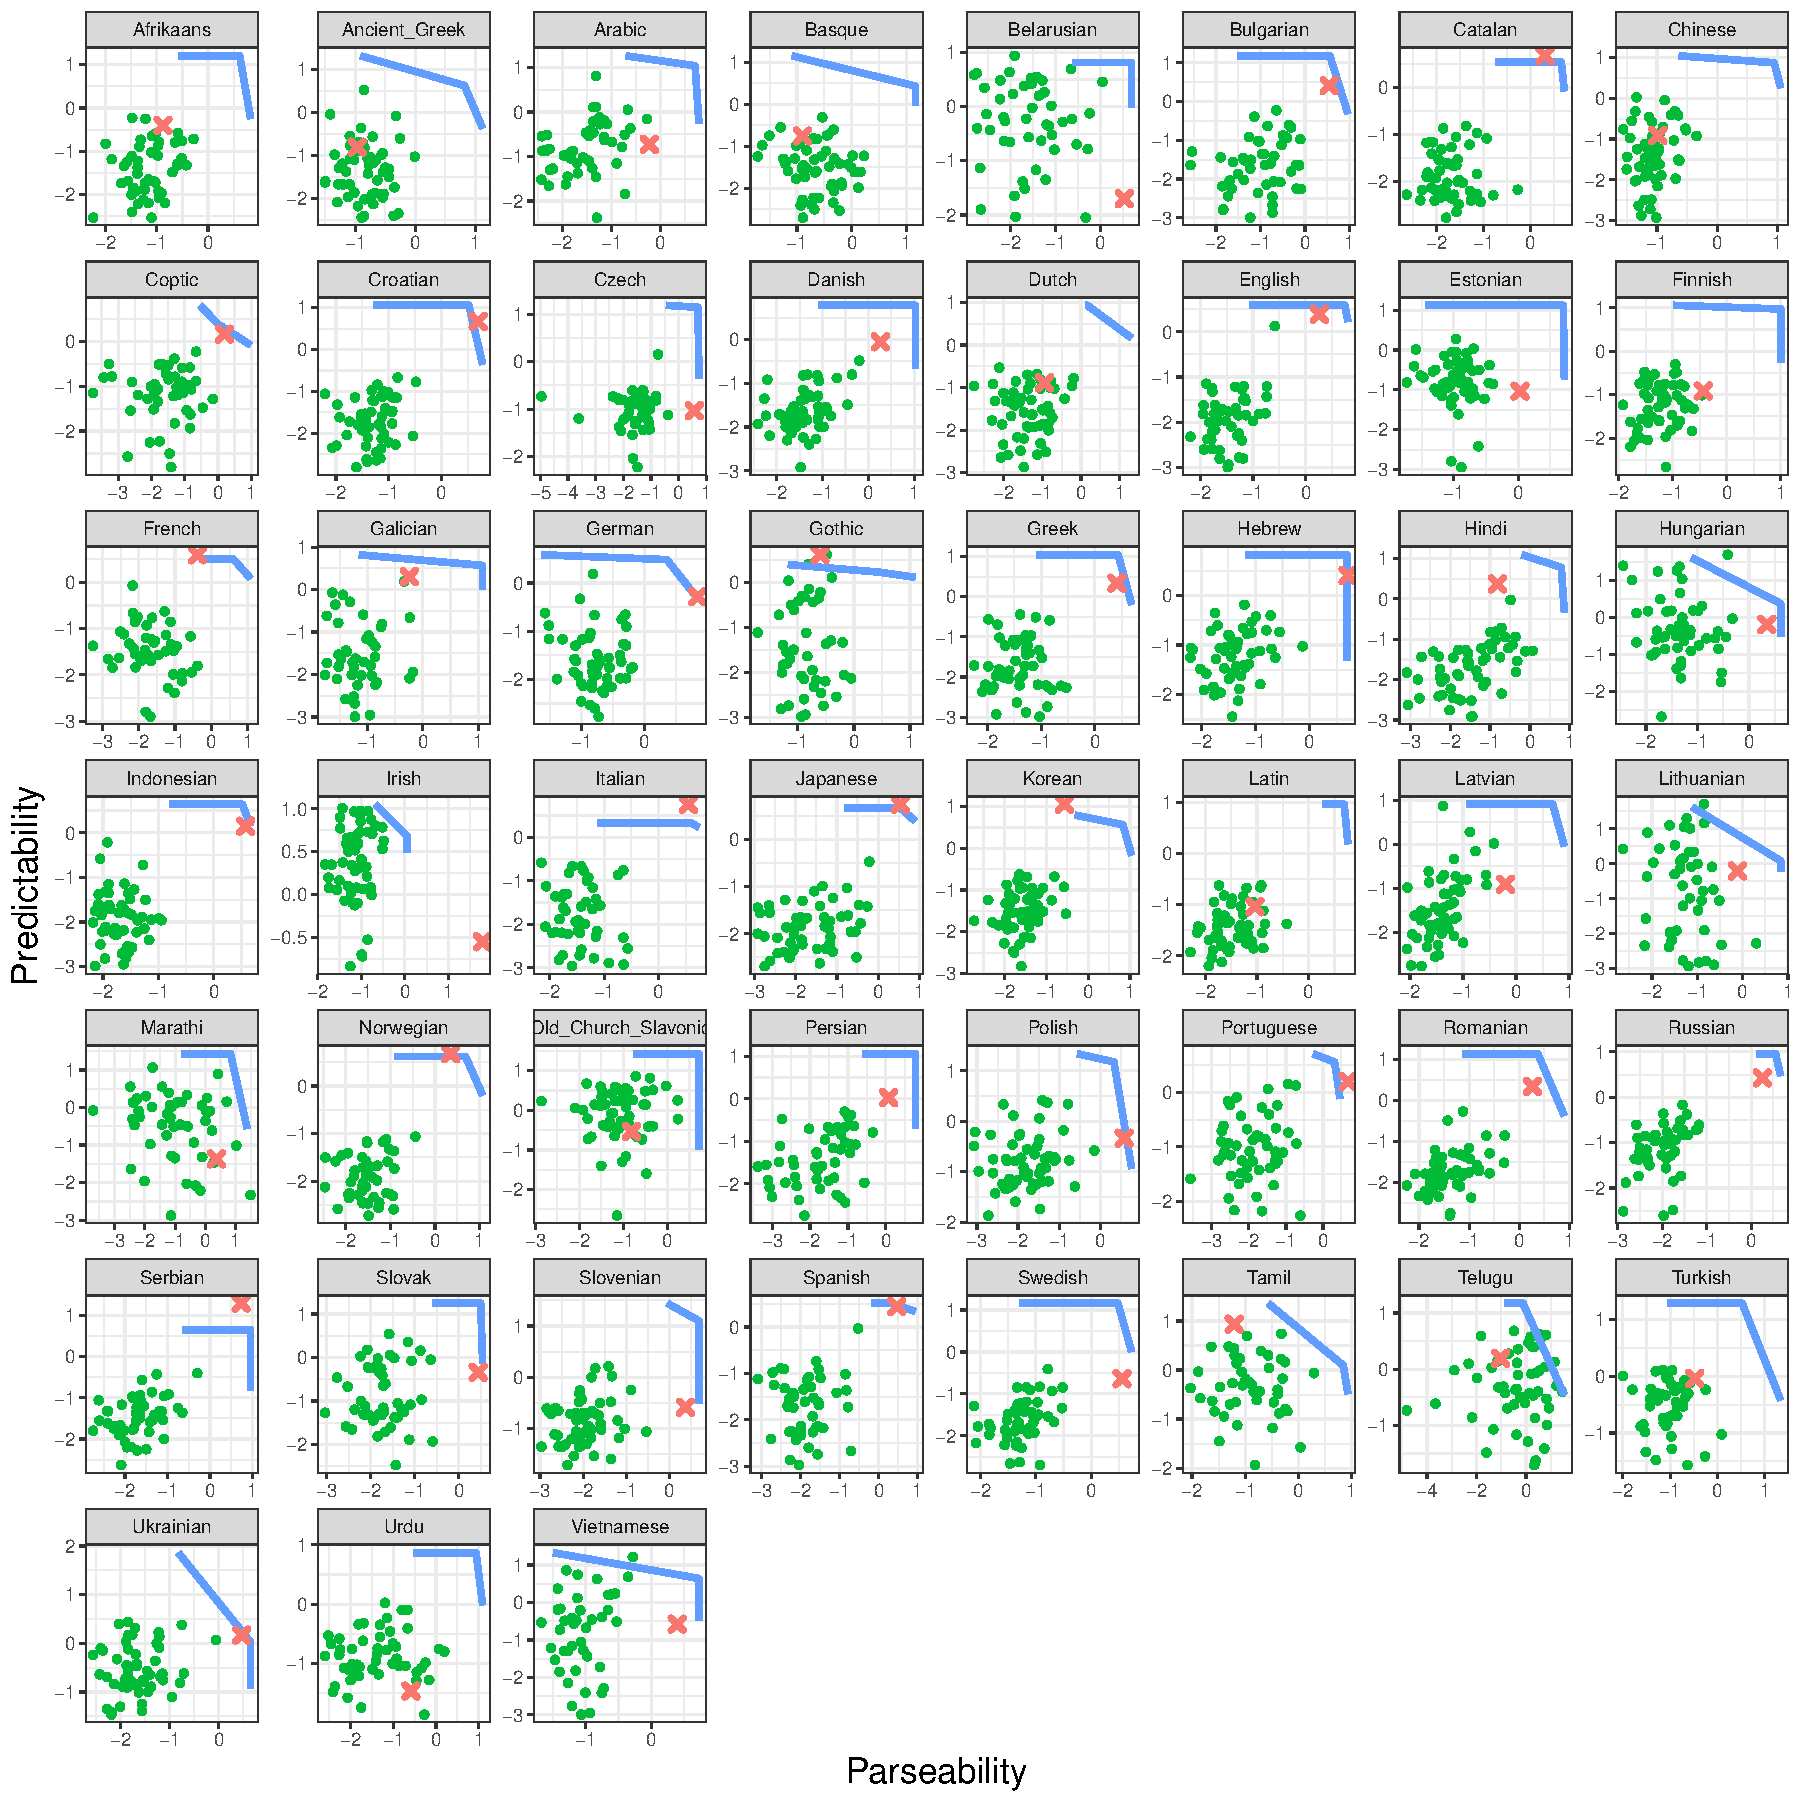
\includegraphics[width=\textwidth]{../results/plane/pareto-plane-perLanguage.pdf}
\caption[Predictability and Parseability]{Predictability and parseability of 51 languages. Green: random baselines, Red: real grammar, blue: approximate Pareto frontier, computed from the optimized grammars.\footnotemark All data are $z$-scored.}\label{fig:pareto-per-lang}
\end{figure}


\begin{figure}
\centering
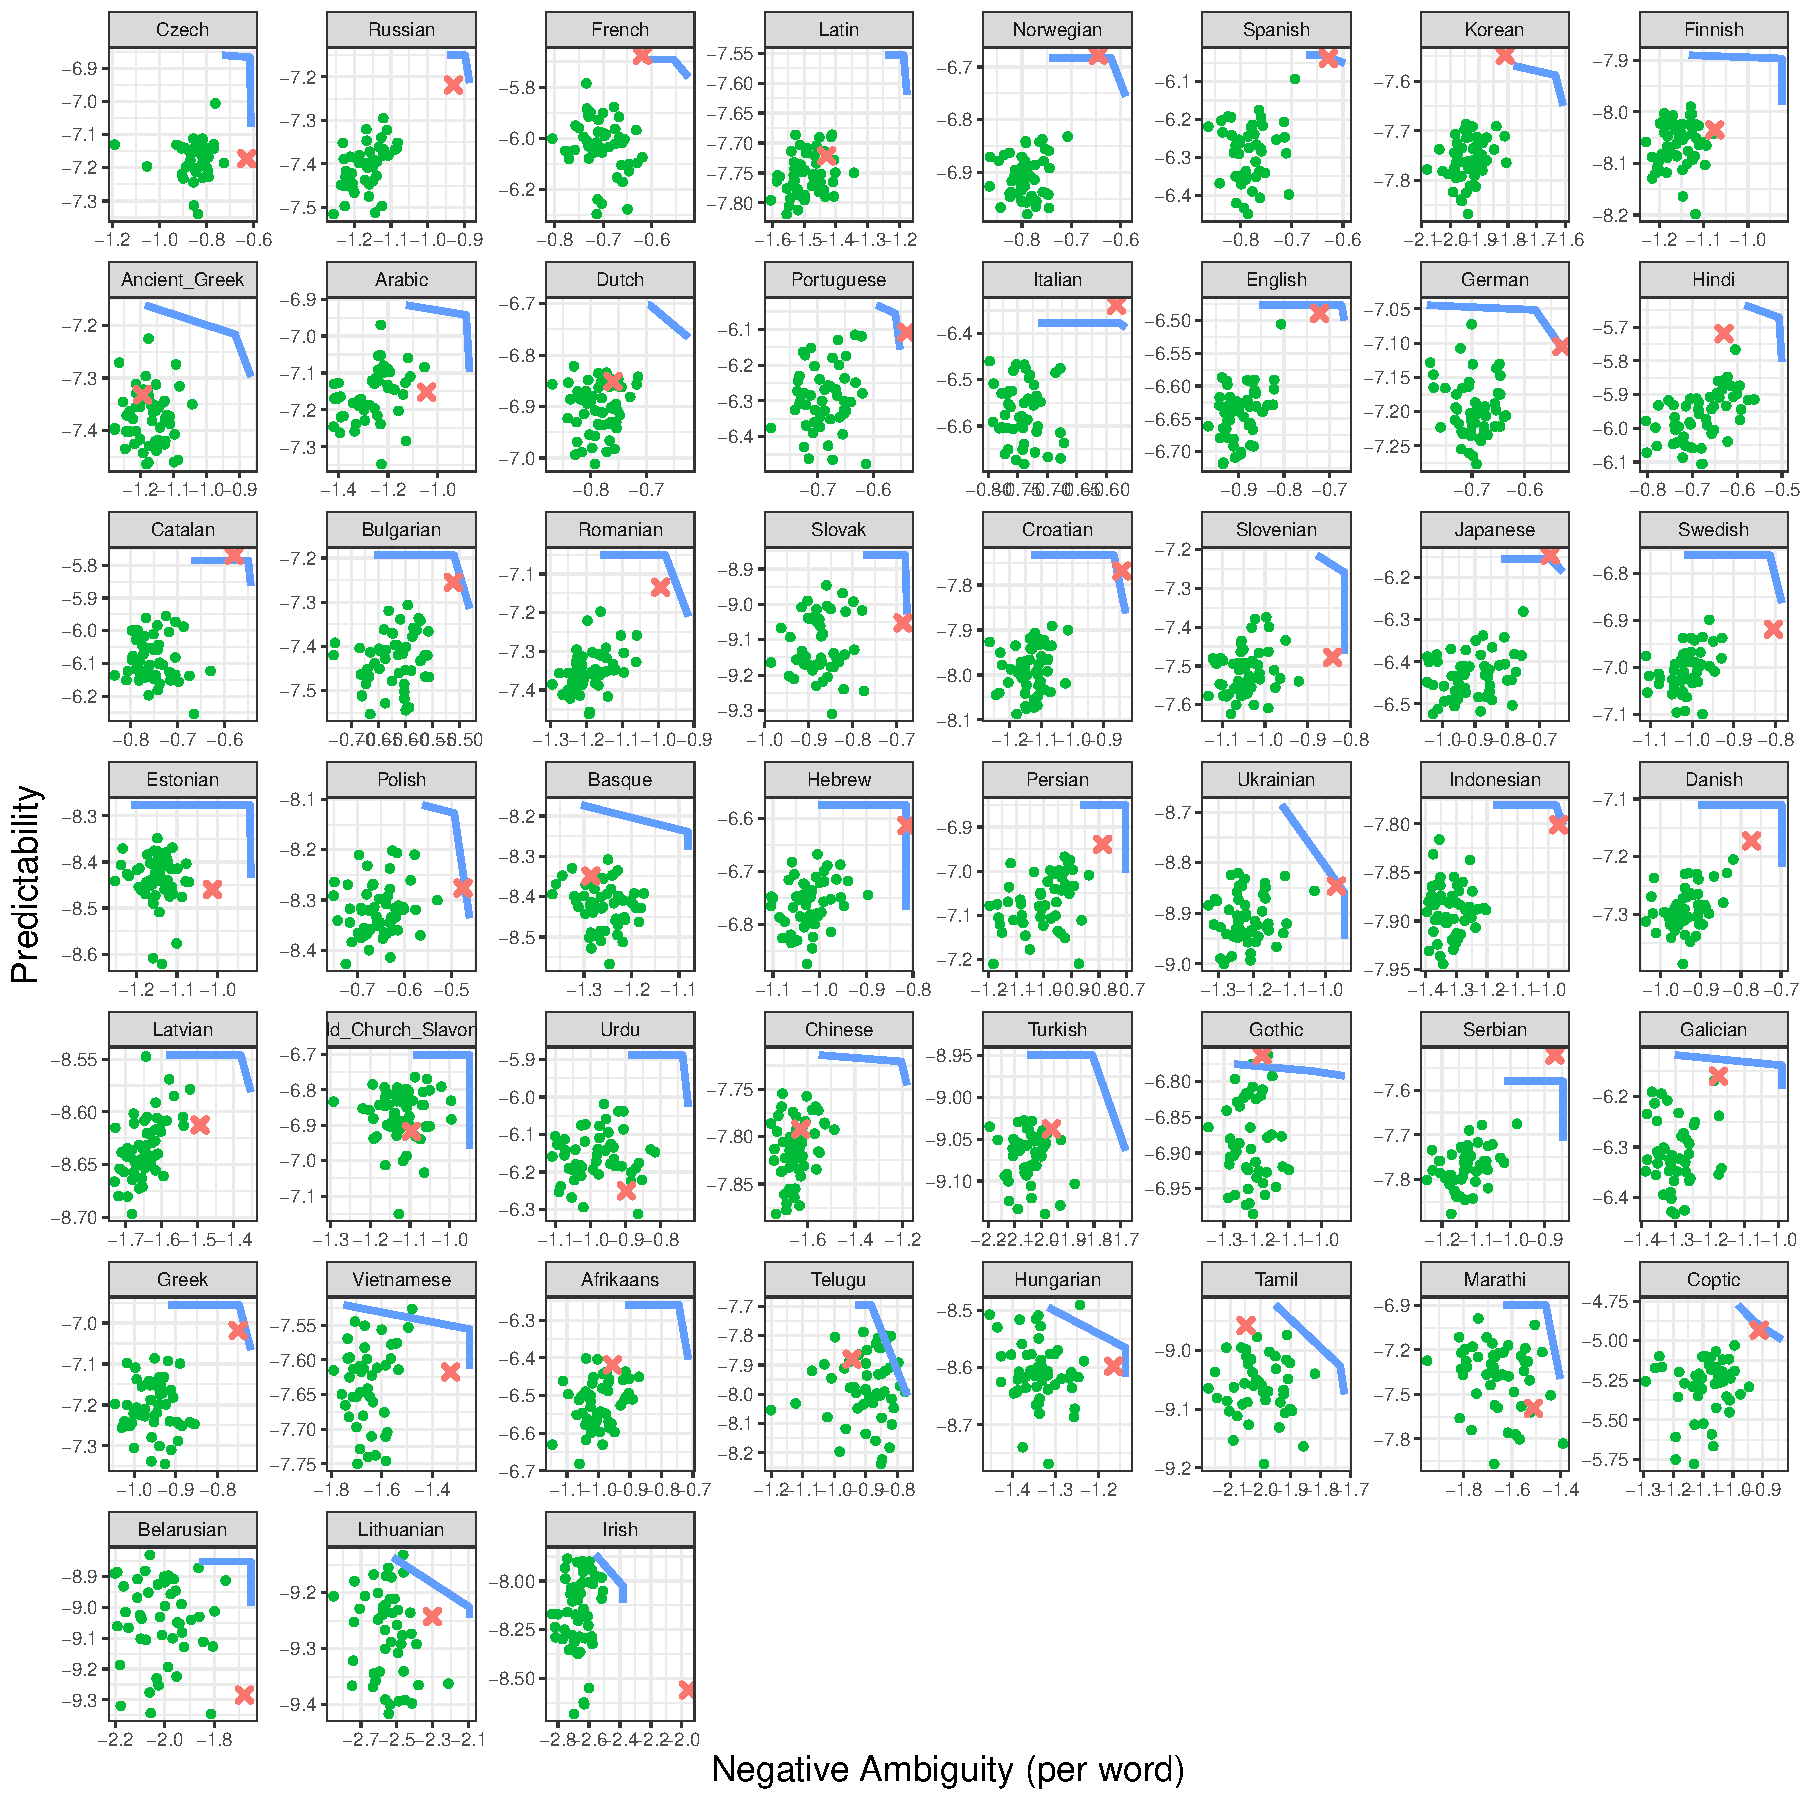
\includegraphics[width=\textwidth]{../results/plane/pareto-plane-perLanguage-raw.pdf}
	\caption[Predictability and Parseability]{Raw numerical values estimated for Predictability (negative surprisal), and negative syntactic ambiguity $-H[T|U]$, before $z$-scoring. For more meaningful comparison, both quantities are normalized by the number of words in the corpus, i.e., we plot per-word negative surprisal and per-word difficulty in recovering syntactic structures.  Note that the negative syntactic ambiguity $-H[T|U]$ equals parseability $I[T,U] = H[T] - H[T|U]$ up to a per-language constant $H[T]$, which we do not attempt to estimate.}\label{fig:pareto-per-lang-raw}
\end{figure}





\footnotetext{Note that, in a few languages, the real grammar is at a position slightly \emph{beyond} the estimated Pareto frontier. This can be attributed to two reasons: First, stochastic gradient descent introduces noise due to its stochasticity and will only approximately find an optimal solution; second, for some corpora, there may be some degree of distributional mismatch between the training partitions (on which grammars are optimized) and held-out partitions (on which efficiency is estimated). This in particular applies to very small corpora such as Irish (121 training sentences).}


In the main paper, we tested whether real grammars are more efficient than the mean of random grammars, using a $t$-test.
We also conducted the analysis using a Binomial test (one-sided), testing whether the real gramar is more efficient than the \emph{median} of random grammars, avoiding any distributional assumption on the random grammars.
As before, we used Hochberg's step-up procedure (Note that the tests for different languages are independent, as different random grammars are evaluated for each language), with $\alpha=0.05$.
In this analysis, real grammars improved in parseability for 80\% of languages, in predictability for 69\% of languages, and in either of both in 92\% of languages ($p<0.05$, with Bonferroni correction).
In Table~\ref{fig:pareto-per-lang-stats}, we provide per-language results for the $t$-tests and binomial tests.




\begin{table}
\centering
\small{
\begin{tabular}{l||ll|lll|lll}
Language & Pred. (t) & Parse. (t) & \multicolumn{3}{c|}{Pred. (Binomial)} & \multicolumn{3}{c}{Parseab. (Binomial)} \\ 
&  $p$ & $p$ &  Est. &CI & $p$ & Est. & CI & $p$  \\ \hline \hline
Afrikaans  & \num{5.29e-13} & \num{9.35e-06} & $0.96$ & $[0.89,1]$ & \num{1.59e-13} & $0.72$ & $[0.6,1]$ & \num{0.000748}\\ 
Ancient Greek  & \num{1.17e-07} & \num{1} & $0.8$ & $[0.69,1]$ & \num{7.01e-06} & $0.29$ & $[0.19,1]$ & \num{0.999}\\ 
Arabic  & \num{0.0774} & \num{<2e-16} & $0.57$ & $[0.44,1]$ & \num{0.196} & $0.96$ & $[0.89,1]$ & \num{4.28e-14}\\ 
Basque  & \num{2.69e-13} & \num{1} & $0.89$ & $[0.79,1]$ & \num{2.9e-09} & $0.24$ & $[0.15,1]$ & \num{1}\\ 
Belarusian  & \num{1} & \num{<2e-16} & $0.14$ & $[0.07,1]$ & \num{1} & $1$ & $[0.95,1]$ & \num{<2e-16}\\ 
Bulgarian  & \num{<2e-16} & \num{<2e-16} & $1$ & $[0.94,1]$ & \num{8.88e-16} & $1$ & $[0.95,1]$ & \num{<2e-16}\\ 
Catalan  & \num{<2e-16} & \num{<2e-16} & $1$ & $[0.95,1]$ & \num{<2e-16} & $1$ & $[0.95,1]$ & \num{<2e-16}\\ 
Chinese  & \num{1.56e-06} & \num{0.00084} & $0.75$ & $[0.64,1]$ & \num{0.000117} & $0.73$ & $[0.62,1]$ & \num{0.000343}\\ 
Coptic  & \num{0.00175} & \num{<2e-16} & $1$ & $[0.94,1]$ & \num{1.78e-15} & $1$ & $[0.95,1]$ & \num{<2e-16}\\ 
Croatian  & \num{<2e-16} & \num{<2e-16} & $1$ & $[0.94,1]$ & \num{4.44e-16} & $1$ & $[0.95,1]$ & \num{<2e-16}\\ 
Czech  & \num{0.438} & \num{<2e-16} & $0.46$ & $[0.34,1]$ & \num{0.756} & $1$ & $[0.94,1]$ & \num{4.44e-16}\\ 
Danish  & \num{<2e-16} & \num{<2e-16} & $1$ & $[0.95,1]$ & \num{<2e-16} & $1$ & $[0.95,1]$ & \num{<2e-16}\\ 
Dutch  & \num{1.41e-11} & \num{1} & $0.87$ & $[0.77,1]$ & \num{6.54e-09} & $0.27$ & $[0.18,1]$ & \num{1}\\ 
English  & \num{<2e-16} & \num{<2e-16} & $1$ & $[0.94,1]$ & \num{1.78e-15} & $1$ & $[0.95,1]$ & \num{<2e-16}\\ 
Estonian  & \num{0.942} & \num{<2e-16} & $0.27$ & $[0.18,1]$ & \num{1} & $1$ & $[0.95,1]$ & \num{<2e-16}\\ 
Finnish  & \num{8.85e-06} & \num{<2e-16} & $0.7$ & $[0.58,1]$ & \num{0.00274} & $1$ & $[0.95,1]$ & \num{<2e-16}\\ 
French  & \num{4.22e-09} & \num{<2e-16} & $1$ & $[0.94,1]$ & \num{8.88e-16} & $0.98$ & $[0.91,1]$ & \num{1.18e-14}\\ 
Galician  & \num{8.48e-15} & \num{<2e-16} & $1$ & $[0.94,1]$ & \num{1.78e-15} & $0.95$ & $[0.87,1]$ & \num{4.07e-13}\\ 
German  & \num{<2e-16} & \num{<2e-16} & $0.98$ & $[0.91,1]$ & \num{1.18e-14} & $1$ & $[0.95,1]$ & \num{<2e-16}\\ 
Gothic  & \num{9.98e-16} & \num{0.64} & $0.98$ & $[0.91,1]$ & \num{6e-15} & $0.48$ & $[0.36,1]$ & \num{0.658}\\ 
Greek  & \num{<2e-16} & \num{<2e-16} & $1$ & $[0.95,1]$ & \num{<2e-16} & $1$ & $[0.95,1]$ & \num{<2e-16}\\ 
Hebrew  & \num{<2e-16} & \num{<2e-16} & $1$ & $[0.95,1]$ & \num{<2e-16} & $1$ & $[0.95,1]$ & \num{<2e-16}\\ 
Hindi  & \num{<2e-16} & \num{1.41e-10} & $1$ & $[0.95,1]$ & \num{<2e-16} & $0.87$ & $[0.77,1]$ & \num{2e-08}\\ 
Hungarian  & \num{0.127} & \num{<2e-16} & $0.66$ & $[0.54,1]$ & \num{0.0135} & $1$ & $[0.95,1]$ & \num{<2e-16}\\ 
Indonesian  & \num{<2e-16} & \num{<2e-16} & $1$ & $[0.95,1]$ & \num{<2e-16} & $1$ & $[0.95,1]$ & \num{<2e-16}\\ 
Irish  & \num{0.982} & \num{<2e-16} & $0.09$ & $[0.04,1]$ & \num{1} & $1$ & $[0.96,1]$ & \num{<2e-16}\\ 
Italian  & \num{<2e-16} & \num{<2e-16} & $1$ & $[0.94,1]$ & \num{4.44e-16} & $1$ & $[0.94,1]$ & \num{4.44e-16}\\ 
Japanese  & \num{<2e-16} & \num{<2e-16} & $1$ & $[0.95,1]$ & \num{<2e-16} & $1$ & $[0.95,1]$ & \num{<2e-16}\\ 
Korean  & \num{<2e-16} & \num{<2e-16} & $1$ & $[0.95,1]$ & \num{<2e-16} & $0.98$ & $[0.92,1]$ & \num{1.55e-15}\\ 
Latin  & \num{3.97e-09} & \num{2.37e-07} & $0.79$ & $[0.67,1]$ & \num{1.79e-05} & $0.8$ & $[0.69,1]$ & \num{7.01e-06}\\ 
Latvian  & \num{1.14e-06} & \num{<2e-16} & $0.76$ & $[0.65,1]$ & \num{5.68e-05} & $1$ & $[0.95,1]$ & \num{<2e-16}\\ 
Lithuanian  & \num{0.000234} & \num{<2e-16} & $0.62$ & $[0.5,1]$ & \num{0.0492} & $0.98$ & $[0.91,1]$ & \num{6e-15}\\ 
Marathi  & \num{1} & \num{<2e-16} & $0.18$ & $[0.1,1]$ & \num{1} & $1$ & $[0.95,1]$ & \num{<2e-16}\\ 
Norwegian  & \num{<2e-16} & \num{<2e-16} & $1$ & $[0.94,1]$ & \num{1.42e-14} & $1$ & $[0.94,1]$ & \num{2.22e-16}\\ 
Old Church Slavonic  & \num{1} & \num{1.6e-05} & $0.19$ & $[0.1,1]$ & \num{1} & $0.73$ & $[0.62,1]$ & \num{0.000343}\\ 
Persian  & \num{<2e-16} & \num{<2e-16} & $1$ & $[0.94,1]$ & \num{2.22e-16} & $1$ & $[0.95,1]$ & \num{<2e-16}\\ 
Polish  & \num{3.57e-08} & \num{<2e-16} & $0.8$ & $[0.69,1]$ & \num{4.35e-06} & $1$ & $[0.95,1]$ & \num{<2e-16}\\ 
Portuguese  & \num{0.00814} & \num{<2e-16} & $1$ & $[0.95,1]$ & \num{<2e-16} & $1$ & $[0.95,1]$ & \num{<2e-16}\\ 
Romanian  & \num{<2e-16} & \num{<2e-16} & $1$ & $[0.95,1]$ & \num{<2e-16} & $1$ & $[0.95,1]$ & \num{<2e-16}\\ 
Russian  & \num{<2e-16} & \num{<2e-16} & $1$ & $[0.94,1]$ & \num{4.44e-16} & $1$ & $[0.95,1]$ & \num{<2e-16}\\ 
Serbian  & \num{<2e-16} & \num{<2e-16} & $1$ & $[0.94,1]$ & \num{2.22e-16} & $1$ & $[0.95,1]$ & \num{<2e-16}\\ 
Slovak  & \num{6.14e-06} & \num{<2e-16} & $0.67$ & $[0.54,1]$ & \num{0.0129} & $1$ & $[0.95,1]$ & \num{<2e-16}\\ 
Slovenian  & \num{1.79e-05} & \num{<2e-16} & $0.8$ & $[0.69,1]$ & \num{7.01e-06} & $1$ & $[0.95,1]$ & \num{<2e-16}\\ 
Spanish  & \num{5.09e-13} & \num{<2e-16} & $1$ & $[0.94,1]$ & \num{8.88e-16} & $1$ & $[0.95,1]$ & \num{<2e-16}\\ 
Swedish  & \num{<2e-16} & \num{<2e-16} & $0.98$ & $[0.91,1]$ & \num{6e-15} & $1$ & $[0.95,1]$ & \num{<2e-16}\\ 
Tamil  & \num{5.43e-13} & \num{<2e-16} & $1$ & $[0.94,1]$ & \num{1.78e-15} & $0.94$ & $[0.86,1]$ & \num{1.46e-12}\\ 
Telugu  & \num{8.2e-07} & \num{0.00797} & $0.8$ & $[0.69,1]$ & \num{7.01e-06} & $0.59$ & $[0.47,1]$ & \num{0.11}\\ 
Turkish  & \num{6.95e-07} & \num{5.06e-16} & $0.88$ & $[0.78,1]$ & \num{1.62e-08} & $0.92$ & $[0.84,1]$ & \num{3.53e-11}\\ 
Ukrainian  & \num{5.79e-15} & \num{<2e-16} & $0.87$ & $[0.77,1]$ & \num{6.54e-09} & $1$ & $[0.95,1]$ & \num{<2e-16}\\ 
Urdu  & \num{1} & \num{4.84e-11} & $0.1$ & $[0.04,1]$ & \num{1} & $0.83$ & $[0.72,1]$ & \num{1.02e-06}\\ 
Vietnamese  & \num{0.00274} & \num{<2e-16} & $0.54$ & $[0.41,1]$ & \num{0.333} & $1$ & $[0.95,1]$ & \num{<2e-16}\\ 

\end{tabular}
}
\caption{Per-language results in Study 1. For each language, we show the following: (1) $p$-values obtained from a one-sided $t$-test, for the null that the mean predictability/parseability of random grammars is at least as high as that of the real grammar. (2) Results from one-sided binomial tests, for the null that the the real grammar is better than at most $50 \%$ of random grammars. In addition to the $p$-value, we report point estimate and 95\% confidence interval for the fraction of random grammars that have values below real grammars.}\label{fig:pareto-per-lang-stats}
\end{table}



\begin{table}
\centering
\small{
\begin{tabular}{l||ll|lll|lll}
Language & Pred. (t) & Parse. (t) & \multicolumn{3}{c|}{Pred. (Binomial)} & \multicolumn{3}{c}{Parseab. (Binomial)} \\ 
&  $p$ & $p$ &  Est. &CI & $p$ & Est. & CI & $p$  \\ \hline \hline
Afrikaans  & \num{0.00945} & \num{0.97} & $1$ & $[0.95,1]$ & \num{<2e-16} & $0.44$ & $[0.33,1]$ & \num{0.83}\\ 
Ancient Greek  & \num{2.4e-10} & \num{1} & $0.84$ & $[0.73,1]$ & \num{2.17e-07} & $0.29$ & $[0.19,1]$ & \num{0.999}\\ 
Arabic  & \num{1} & \num{<2e-16} & $0.04$ & $[0.01,1]$ & \num{1} & $0.96$ & $[0.89,1]$ & \num{4.28e-14}\\ 
Basque  & \num{6.39e-12} & \num{1} & $0.93$ & $[0.84,1]$ & \num{1.02e-11} & $0.27$ & $[0.18,1]$ & \num{1}\\ 
Belarusian  & \num{0.0417} & \num{<2e-16} & $0.56$ & $[0.44,1]$ & \num{0.209} & $1$ & $[0.95,1]$ & \num{<2e-16}\\ 
Bulgarian  & \num{<2e-16} & \num{<2e-16} & $1$ & $[0.95,1]$ & \num{<2e-16} & $1$ & $[0.95,1]$ & \num{<2e-16}\\ 
Catalan  & \num{1.27e-05} & \num{<2e-16} & $1$ & $[0.95,1]$ & \num{<2e-16} & $1$ & $[0.95,1]$ & \num{<2e-16}\\ 
Chinese  & \num{0.000172} & \num{0.00271} & $0.66$ & $[0.54,1]$ & \num{0.0111} & $0.73$ & $[0.62,1]$ & \num{0.000343}\\ 
Coptic  & \num{4.06e-06} & \num{<2e-16} & $0.85$ & $[0.75,1]$ & \num{6.92e-08} & $1$ & $[0.95,1]$ & \num{<2e-16}\\ 
Croatian  & \num{<2e-16} & \num{<2e-16} & $1$ & $[0.95,1]$ & \num{<2e-16} & $1$ & $[0.95,1]$ & \num{<2e-16}\\ 
Czech  & \num{<2e-16} & \num{3.41e-12} & $1$ & $[0.94,1]$ & \num{2.22e-16} & $1$ & $[0.83,1]$ & \num{1.53e-05}\\ 
Danish  & \num{<2e-16} & \num{<2e-16} & $1$ & $[0.95,1]$ & \num{<2e-16} & $1$ & $[0.95,1]$ & \num{<2e-16}\\ 
Dutch  & \num{<2e-16} & \num{<2e-16} & $0.98$ & $[0.92,1]$ & \num{1.55e-15} & $0.96$ & $[0.89,1]$ & \num{4.28e-14}\\ 
English  & \num{<2e-16} & \num{<2e-16} & $1$ & $[0.95,1]$ & \num{<2e-16} & $1$ & $[0.95,1]$ & \num{<2e-16}\\ 
Estonian  & \num{<2e-16} & \num{<2e-16} & $1$ & $[0.95,1]$ & \num{<2e-16} & $1$ & $[0.95,1]$ & \num{<2e-16}\\ 
Finnish  & \num{3.92e-13} & \num{<2e-16} & $0.92$ & $[0.84,1]$ & \num{3.53e-11} & $1$ & $[0.95,1]$ & \num{<2e-16}\\ 
French  & \num{7.81e-08} & \num{<2e-16} & $1$ & $[0.95,1]$ & \num{<2e-16} & $1$ & $[0.95,1]$ & \num{<2e-16}\\ 
Galician  & \num{0.343} & \num{<2e-16} & $0.18$ & $[0.1,1]$ & \num{1} & $0.98$ & $[0.92,1]$ & \num{7.91e-16}\\ 
German  & \num{8.14e-16} & \num{<2e-16} & $0.93$ & $[0.84,1]$ & \num{5.5e-12} & $1$ & $[0.95,1]$ & \num{<2e-16}\\ 
Gothic  & \num{1} & \num{0.332} & $0.07$ & $[0.03,1]$ & \num{1} & $0.57$ & $[0.45,1]$ & \num{0.17}\\ 
Greek  & \num{<2e-16} & \num{<2e-16} & $1$ & $[0.95,1]$ & \num{<2e-16} & $1$ & $[0.95,1]$ & \num{<2e-16}\\ 
Hebrew  & \num{0.000744} & \num{<2e-16} & $1$ & $[0.95,1]$ & \num{<2e-16} & $1$ & $[0.95,1]$ & \num{<2e-16}\\ 
Hindi  & \num{<2e-16} & \num{1.32e-15} & $1$ & $[0.95,1]$ & \num{<2e-16} & $0.91$ & $[0.82,1]$ & \num{1.95e-10}\\ 
Hungarian  & \num{1.28e-07} & \num{<2e-16} & $0.79$ & $[0.68,1]$ & \num{1.12e-05} & $1$ & $[0.95,1]$ & \num{<2e-16}\\ 
Indonesian  & \num{<2e-16} & \num{<2e-16} & $0.98$ & $[0.92,1]$ & \num{1.55e-15} & $1$ & $[0.95,1]$ & \num{<2e-16}\\ 
Italian  & \num{9.09e-11} & \num{<2e-16} & $1$ & $[0.94,1]$ & \num{4.44e-16} & $1$ & $[0.94,1]$ & \num{8.88e-16}\\ 
Japanese  & \num{<2e-16} & \num{<2e-16} & $1$ & $[0.95,1]$ & \num{<2e-16} & $1$ & $[0.95,1]$ & \num{<2e-16}\\ 
Korean  & \num{<2e-16} & \num{6.52e-13} & $0.98$ & $[0.92,1]$ & \num{1.55e-15} & $0.87$ & $[0.77,1]$ & \num{1.15e-08}\\ 
Latin  & \num{4.92e-11} & \num{<2e-16} & $0.85$ & $[0.75,1]$ & \num{6.92e-08} & $0.98$ & $[0.92,1]$ & \num{3.05e-15}\\ 
Latvian  & \num{0.0107} & \num{<2e-16} & $0.52$ & $[0.4,1]$ & \num{0.446} & $1$ & $[0.95,1]$ & \num{<2e-16}\\ 
Lithuanian  & \num{5.64e-05} & \num{1.4e-12} & $0.75$ & $[0.64,1]$ & \num{0.000134} & $0.91$ & $[0.81,1]$ & \num{3.54e-10}\\ 
Marathi  & \num{1.07e-05} & \num{8.79e-09} & $0.74$ & $[0.62,1]$ & \num{0.000268} & $0.78$ & $[0.66,1]$ & \num{2.6e-05}\\ 
Norwegian  & \num{<2e-16} & \num{<2e-16} & $1$ & $[0.94,1]$ & \num{2.22e-16} & $1$ & $[0.94,1]$ & \num{2.22e-16}\\ 
Old Church Slavonic  & \num{<2e-16} & \num{4.93e-13} & $0.96$ & $[0.89,1]$ & \num{2.22e-14} & $0.89$ & $[0.8,1]$ & \num{5.09e-10}\\ 
Persian  & \num{<2e-16} & \num{<2e-16} & $0.94$ & $[0.86,1]$ & \num{2.76e-12} & $1$ & $[0.95,1]$ & \num{<2e-16}\\ 
Polish  & \num{1.4e-05} & \num{<2e-16} & $0.73$ & $[0.61,1]$ & \num{0.000508} & $1$ & $[0.95,1]$ & \num{<2e-16}\\ 
Portuguese  & \num{0.0269} & \num{<2e-16} & $1$ & $[0.95,1]$ & \num{<2e-16} & $1$ & $[0.95,1]$ & \num{<2e-16}\\ 
Romanian  & \num{<2e-16} & \num{<2e-16} & $1$ & $[0.95,1]$ & \num{<2e-16} & $1$ & $[0.95,1]$ & \num{<2e-16}\\ 
Russian  & \num{<2e-16} & \num{<2e-16} & $1$ & $[0.95,1]$ & \num{<2e-16} & $1$ & $[0.95,1]$ & \num{<2e-16}\\ 
Serbian  & \num{<2e-16} & \num{<2e-16} & $1$ & $[0.95,1]$ & \num{<2e-16} & $1$ & $[0.95,1]$ & \num{<2e-16}\\ 
Slovak  & \num{<2e-16} & \num{<2e-16} & $0.93$ & $[0.84,1]$ & \num{1.9e-11} & $1$ & $[0.95,1]$ & \num{<2e-16}\\ 
Slovenian  & \num{<2e-16} & \num{<2e-16} & $0.98$ & $[0.91,1]$ & \num{1.18e-14} & $1$ & $[0.95,1]$ & \num{<2e-16}\\ 
Spanish  & \num{1.87e-12} & \num{<2e-16} & $1$ & $[0.95,1]$ & \num{<2e-16} & $1$ & $[0.95,1]$ & \num{<2e-16}\\ 
Swedish  & \num{<2e-16} & \num{<2e-16} & $1$ & $[0.95,1]$ & \num{<2e-16} & $1$ & $[0.95,1]$ & \num{<2e-16}\\ 
Tamil  & \num{0.0113} & \num{0.000641} & $0.58$ & $[0.46,1]$ & \num{0.136} & $0.7$ & $[0.59,1]$ & \num{0.00192}\\ 
Telugu  & \num{<2e-16} & \num{1.95e-15} & $1$ & $[0.95,1]$ & \num{<2e-16} & $0.93$ & $[0.84,1]$ & \num{1.9e-11}\\ 
Turkish  & \num{0.711} & \num{<2e-16} & $0.47$ & $[0.35,1]$ & \num{0.708} & $0.96$ & $[0.89,1]$ & \num{1.59e-13}\\ 
Ukrainian  & \num{<2e-16} & \num{<2e-16} & $0.98$ & $[0.92,1]$ & \num{1.55e-15} & $1$ & $[0.95,1]$ & \num{<2e-16}\\ 
Urdu  & \num{0.0205} & \num{1.63e-14} & $1$ & $[0.94,1]$ & \num{4.44e-16} & $0.88$ & $[0.78,1]$ & \num{5.16e-09}\\ 
Vietnamese  & \num{1} & \num{<2e-16} & $0.02$ & $[0,1]$ & \num{1} & $1$ & $[0.95,1]$ & \num{<2e-16}\\ 

\end{tabular}
}
	\caption{Per-language results in Study 1, with \emph{lexicalized} parsers and word-level-only language models. Compare Table~\ref{fig:pareto-per-lang-stats}}
\end{table}





\section{Supplementary Analyses for Study 2}
\subsection{Correlation between Universals and Efficiency}

In Figure~\ref{fig:corr-eff-corr}, we plot efficiency, parseability, and predictability (all are $z$-scored within language, as in Study 1) as a function of the number of satisfied correlations, for the real grammars of the 51 languages.

We found very similar results using Spearman's rank correlation (Efficiency: $\rho=0.59$, $p = 9.8 \cdot 10^{-6}$; Parseability: $\rho=0.55$, $p=4.7 \cdot 10^{-5}$; Predictability: $\rho=0.36$, $p=0.012$).


\begin{figure}[ht]
    \centering
    
    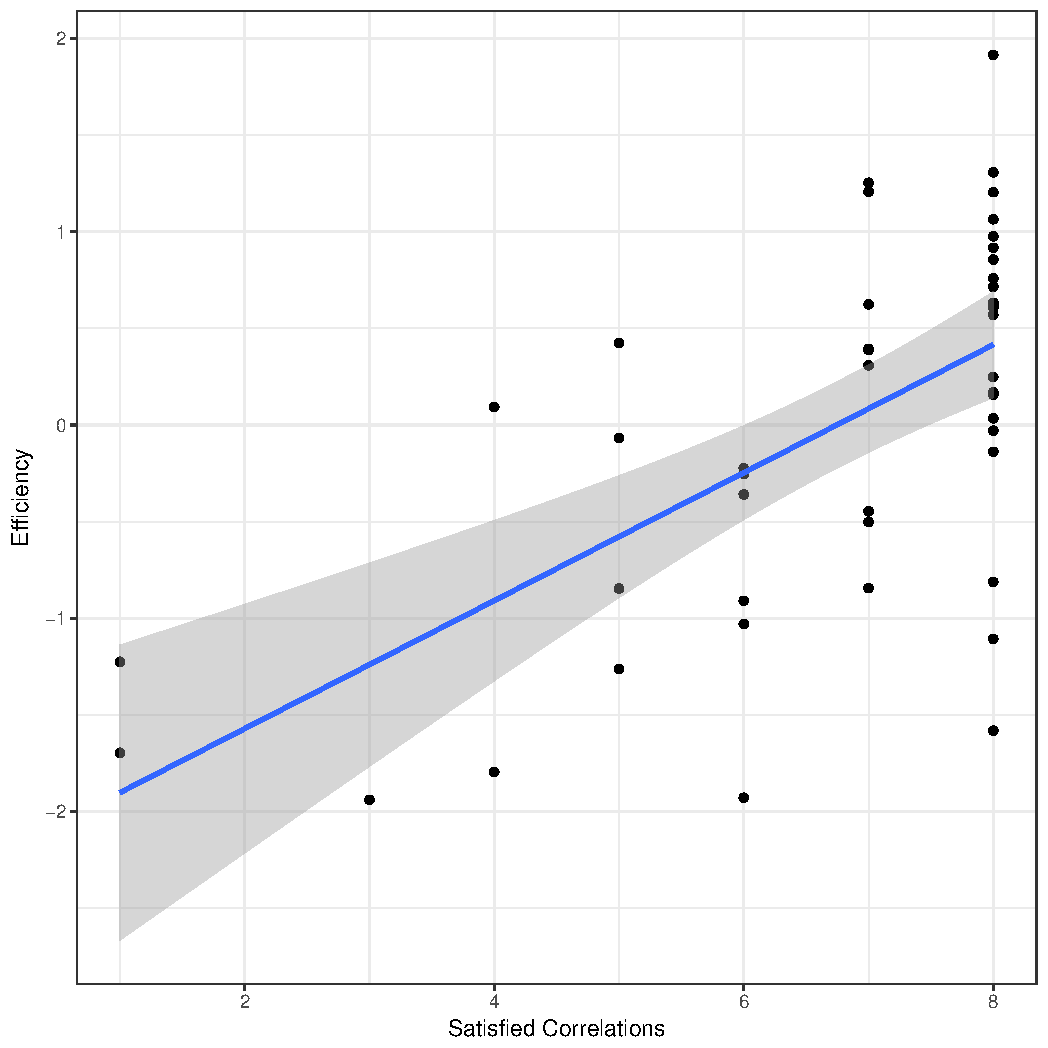
\includegraphics[scale=.55]{../results/correlations/correlations-by-grammar/ground-corrs-efficiency.pdf}
    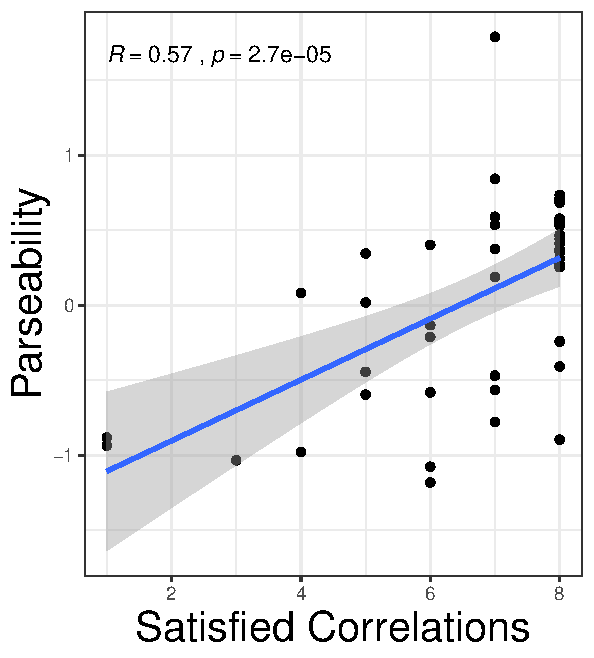
\includegraphics[scale=.55]{../results/correlations/correlations-by-grammar/ground-corrs-parseability.pdf}
    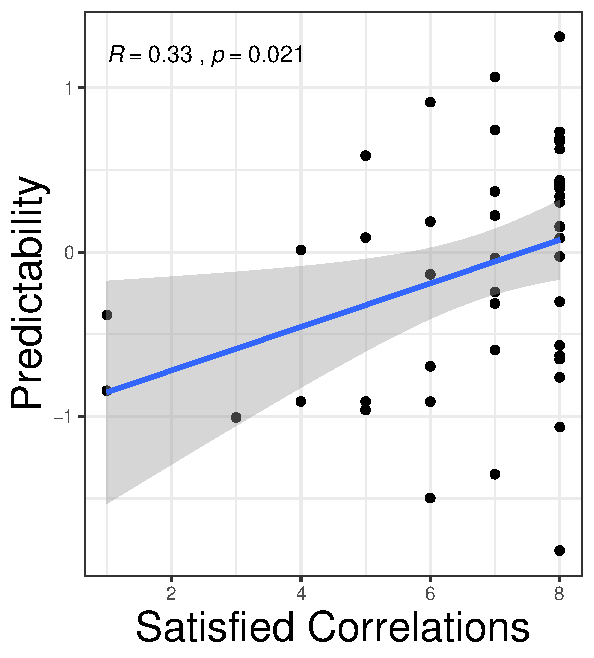
\includegraphics[scale=.55]{../results/correlations/correlations-by-grammar/ground-corrs-predictability.pdf}

	\caption{Correlation between the number of satisfied correlations ($x$-axis) and efficiency, parseability, and predictability ($y$-axis), for the 51 real languages.}
    \label{fig:corr-eff-corr}
\end{figure}



\subsection{Predictions for Individual Languages}


We show predictions for the eight correlations on the level of individual languages in Figure~\ref{fig:per-lang}.
We obtained these predictions for individual languages and each of the eight relations as follows.
For each language and each of the objective functions (efficiency, predictability, parseability), we considered the optimized grammar that yielded the best value of this objective function among the eight optimized grammars (i.e., the grammar where the optimization procedure had been most successful).
We interpreted this grammar as verb-object or object-verb depending on the order in the real grammar of the language.


\begin{figure} 
	\begin{center}
	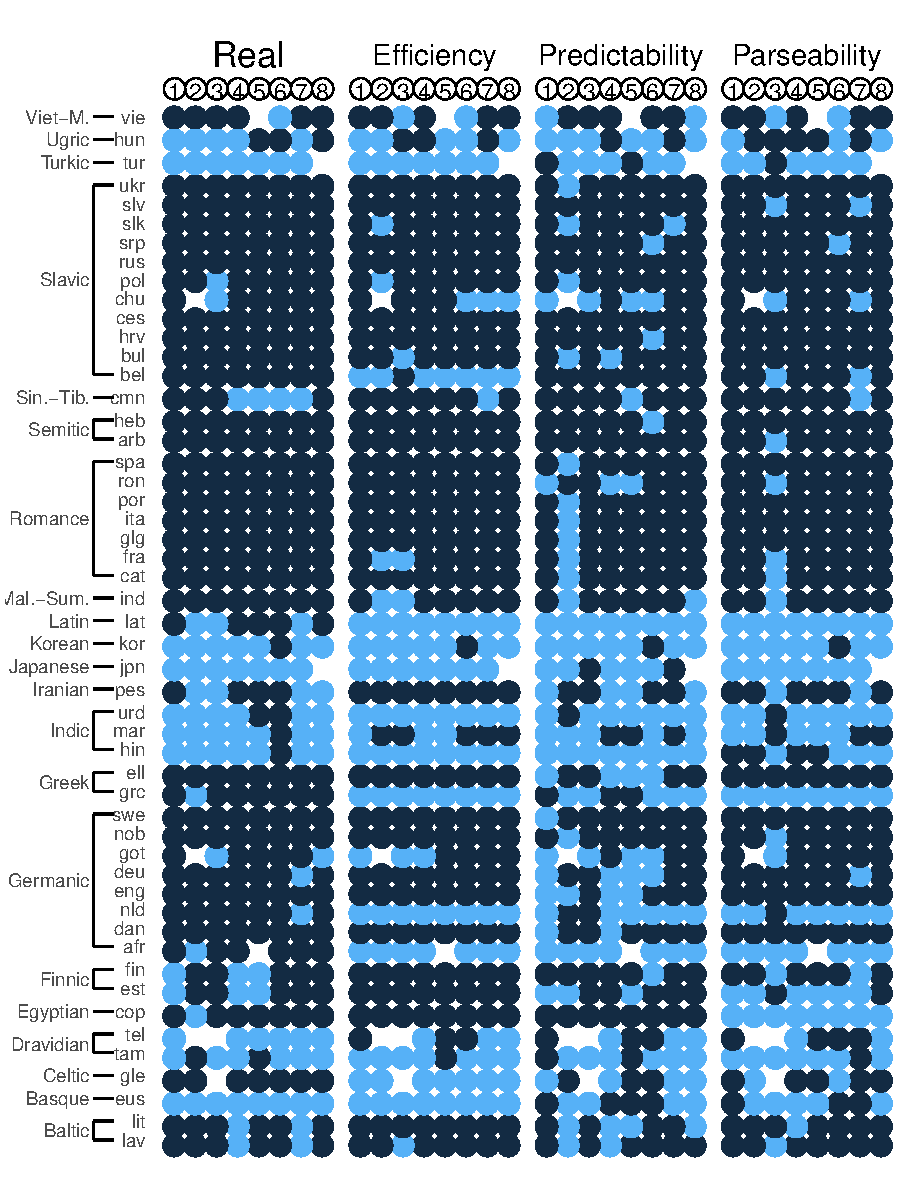
\includegraphics[width=0.7\textwidth]{../results/correlations/figures/pred-eff-pred-pars-families-2.pdf} % figures/pred-eff-families-2.pdf
	\end{center}
	\caption{Order of the eight correlates across 51 languages, in the real grammars (left) and predicted by optimizing for efficiency, predictability, parseability (right). Dark blue: Verb patterner \emph{precedes} object patterner (English, Arabic, ...). Light blue: Verb patterner \emph{follows} object patterner (Japanese, Hindi , ...). White cells indicate that the relation is not annotated in the dataset for the given language.}\label{fig:per-lang}
%	\caption{Order of the eight correlates across 51 languages, in the real grammars (left) and predicted by efficiency optimization (right). Dark blue: Verb patterner \emph{precedes} object patterner(English, Arabic, ...). Light blue: Verb patterner \emph{follows} object patterner (Japanese, Hindi , ...) .}\label{fig:per-lang}
\end{figure}

\subsection{Regression for Predicted Correlations}


%https://github.com/stan-dev/stan/wiki/Prior-Choice-Recommendations

\paragraph{Bayesian Mixed-Effects Regression}
We modeled the probabilities $p_{L,j}$ that a grammar optimized for data from language $L$ satisfies the $j$-th correlation ($j=1,...,8$) using a multilevel logistic model \cite{gelman2013bayesian}, with random intercepts for the language for whose data the grammar had been optimized, and for its language family, annotated according to \url{http://universaldependencies.org/}.
Formally,
\begin{equation}\label{eq:mixed-effects}
logit(p_{L,j}) = \alpha_j + u_{L,j} + v_{f_L,j}
\end{equation}
where $f_L$ is the language family of $L$.
The intercepts $\alpha_j$ ($j=1,...8$) encode the population-level prevalence of the correlations when controlling for differences between datasets from different languages and language families; $u_{L,j}$, $v_{f_L,j}$ encode per-language and per-family deviations from the population-level intercept $\alpha_j$.
%, and
%$u_{L,1,...8} \sim \mathcal{N}(0, \Sigma_{lang})$,
%$v_{f_L,1,...8} \sim \mathcal{N}(0, \Sigma_{fam})$.

%As we constructed 4 verb-object and 4 object-verb grammars for each of the 51 languages, TODO...


Following the recommendations of \cite{ghosh2018use, burkner2018advanced}, we used as a very weakly informative prior a Student's $t$ prior with $\nu=3$ degrees of freedom, mean 0, and scale $\sigma=10$ (i.e., the PDF $p$ is $\frac{1}{\sigma} p_3(x/\sigma)$, where $p_3$ is the PDF of the $t$-distribution with $\nu=3$).
We used this prior for $\alpha_j, \sigma_{L,j}, \tau_{L,j}$.
A correlation that holds in 90\% of cases would correspond to an intercept $\alpha \approx 2.19$ in the logistic model, well within the main probability mass of the prior.

We modeled full covariance matrices of per-language and per-family random intercepts over all eight correlations. We placed an LKJ prior ($\eta=1$) on these matrices, as described in \cite{burkner2018advanced}.
We used MCMC sampling implemented in Stan \cite{carpenter2017stan, hoffman2014no} using the R package \texttt{brms} \cite{buerkner2017brms}.
We ran four chains, with 5000 samples each, of which the first 2500 were discarded as warmup samples.
We confirmed convergence using $\hat{R}$ and visual inspection of chains \cite{gelman2013bayesian}.

We obtained the posterior density plots in Table 2 (Main Paper) and in Figure (\ref{tab:all-predictions-1}) by applying the logistic transformation ($x \mapsto \frac{1}{1+\exp(-x)}$) to the posterior samples of $\alpha_j$ (\ref{eq:mixed-effects}).
As the logistic transformation is inverse to the logit transform (\ref{eq:mixed-effects}), this corresponds to the posterior distribution of the prevalence (between 0.0 and 1.0) of each correlation, controlling for languages and language families.






\paragraph{Robustness}
To ascertain the robustness of our results, we also conducted a frequentist analysis using \texttt{lme4} \cite{bates2015fitting}.
For each of the correlations, we conducted a logistic mixed-effects analysis predicting whether a grammar satisfies the correlation, with random effects of language and language family.
The results are shown in Table~\ref{tab:corr-regression} together with those of the Bayesian analysis.
The frequentist analysis agrees with the Bayesian model; all eight correlations are predicted to hold in more than half of the optimized grammars ($p < 0.01$ each).

Note that the Bayesian analysis  also estimates a posterior distribution of the number of satisfied correlations (see Figure~\ref{fig:posterior}), providing an elegant solution to the multiple-comparisons problem arising from analysing the eight correlation.

% and obtaining $p$-values from the resulting fit: For all eight correlations, the sign of $\alpha$ was positive ($p < 0.05$).


%We obtained qualitatively equivalent results for analyses on the levels of individual relations when estimating frequentist models individually for each correlation using \texttt{lme4} \cite{bates2015fitting} and obtaining $p$-values from the resulting fit: For all eight correlations, the sign of $\alpha$ was positive ($p < 0.05$).


\begin{table}
\small{
\begin{center}
\begin{tabular}{|l||l|lll|llll|ll|llllll}
\hline
 & Prevalence & \multicolumn{3}{c|}{Bayesian} & \multicolumn{4}{c|}{Frequentist} \\ 
& & Mean & SD & $p(\beta \leq 0)$ & $\beta$ & SE & $z$ & p \\
\hline\hline
	\raisebox{.5pt}{\textcircled{\raisebox{-.9pt} {1}}} & 0.779 & 1.449 & 0.273 & $<$ \num{1e-4} & 1.395 & 0.222 & 6.277 & \num{3.5e-10}\\
\raisebox{.5pt}{\textcircled{\raisebox{-.9pt} {2}}} & 0.678 & 0.761 & 0.171 & \num{1.0e-04} & 0.784 & 0.135 & 5.796 & \num{6.8e-09}\\
\raisebox{.5pt}{\textcircled{\raisebox{-.9pt} {3}}} & 0.696 & 1.003 & 0.424 & 0.012 & 0.943 & 0.342 & 2.753 & 0.006\\
\raisebox{.5pt}{\textcircled{\raisebox{-.9pt} {4}}} & 0.782 & 1.586 & 0.318 & $<$ \num{1e-4} & 1.512 & 0.251 & 6.013 & \num{1.8e-09}\\
\raisebox{.5pt}{\textcircled{\raisebox{-.9pt} {5}}} & 0.793 & 1.505 & 0.327 & $<$ \num{1e-4} & 1.434 & 0.272 & 5.281 & \num{1.3e-07}\\
\raisebox{.5pt}{\textcircled{\raisebox{-.9pt} {6}}} & 0.757 & 1.133 & 0.43 & 0.006 & 1.072 & 0.352 & 3.041 & 0.002\\
\raisebox{.5pt}{\textcircled{\raisebox{-.9pt} {7}}} & 0.748 & 1.093 & 0.388 & 0.003 & 1.026 & 0.322 & 3.185 & 0.001\\
\raisebox{.5pt}{\textcircled{\raisebox{-.9pt} {8}}} & 0.911 & 3.854 & 0.878 & $<$ \num{1e-4} & 3.823 & 0.782 & 4.887 & \num{1.0e-06}\\

\hline
\end{tabular}
\end{center}
}
	\caption{Detailed results for Bayesian and Frequentist mixed-effects analyses for the eight correlations. 
We show (1) the raw prevalence of each correlation in the optimized grammars (8 grammars for each of the 51 languages),
(2) for the Bayesian analysis, we provide posterior mean and SD of $\beta$, and the posterior probability that $\beta$ has the opposite sign,
(3) for the Frequentist analysis, we provide the point estimate, SE, $z$, and $p$-values (2-sided).
The frequentist analysis confirms the results of the Bayesian analysis.
}\label{tab:corr-regression}
\end{table}




\paragraph{Comparison to other Formalizations}

Greenberg's original correlations/implications % ?? TODO

\cite{justeson1990explanation} conducted a log-linear analysis on typological judgments of 147 languages, constructing an undirected graphical model.
For the relations examined here, beyond correlations with verb-object order, they found additional correlations between G-N, N-Adp and between Rel-N, N-Adp.
With their model, they found no evidence for a direct correlation V-O, G-N.


\subsection{Comparing Efficiency to its Components}\label{sec:posterior-number}


In Figure~\ref{fig:posterior}, we plot the posterior distribution of the number of correlations predicted to hold in most optimized grammars, as obtained from the Bayesian regression.
For each posterior sample, we say that the $j$-th correlation holds if the value of $\alpha_j$ in that posterior sample is positive.
In the figure, we plot the fraction of posterior samples in which a given number of correlations is satisfied.
In addition to grammars optimized for efficiency, we also report the result for grammars optimized for predictability and for parseability alone.
Efficiency predicts all eight correlations with high posterior probability; predictability and parseability alone do not.

\begin{figure}[ht]
	\begin{center}
	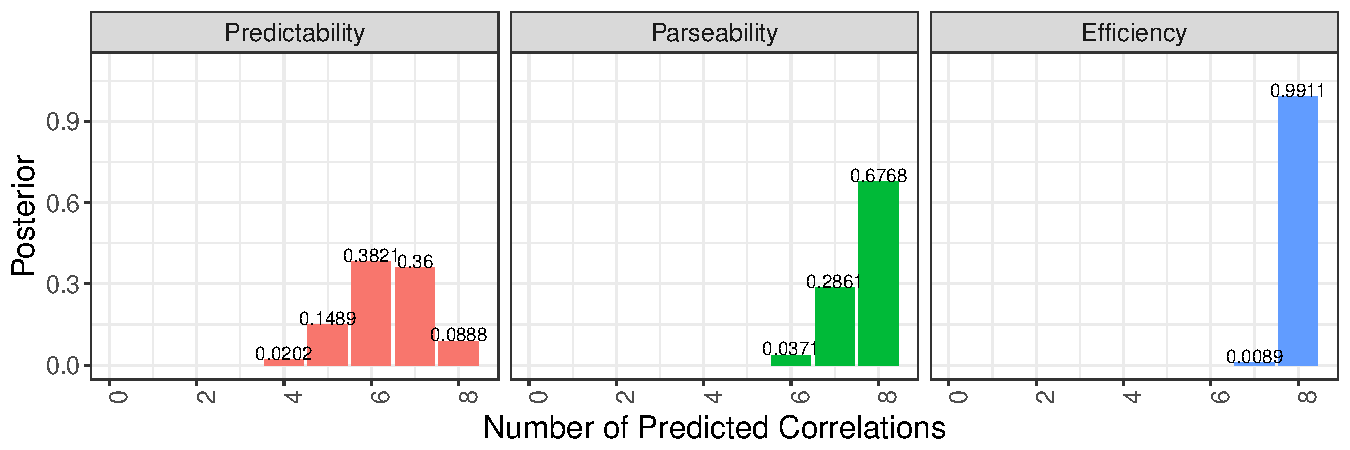
\includegraphics[width=0.98\textwidth]{../results/correlations/figures/posterior-satisfied-universals-together-large-three.pdf}
	\end{center}
	\caption{Posterior of the number of correlations correctly predicted by efficiency and its components, in the Bayesian multivariate mixed-effects logistic regression with random effects for languages and language families. We show results for grammars optimized for only Predictability (left), only Parseability (center), and full Efficiency (right).}\label{fig:posterior}
\end{figure}


%\begin{figure}
%    \centering
%    
%    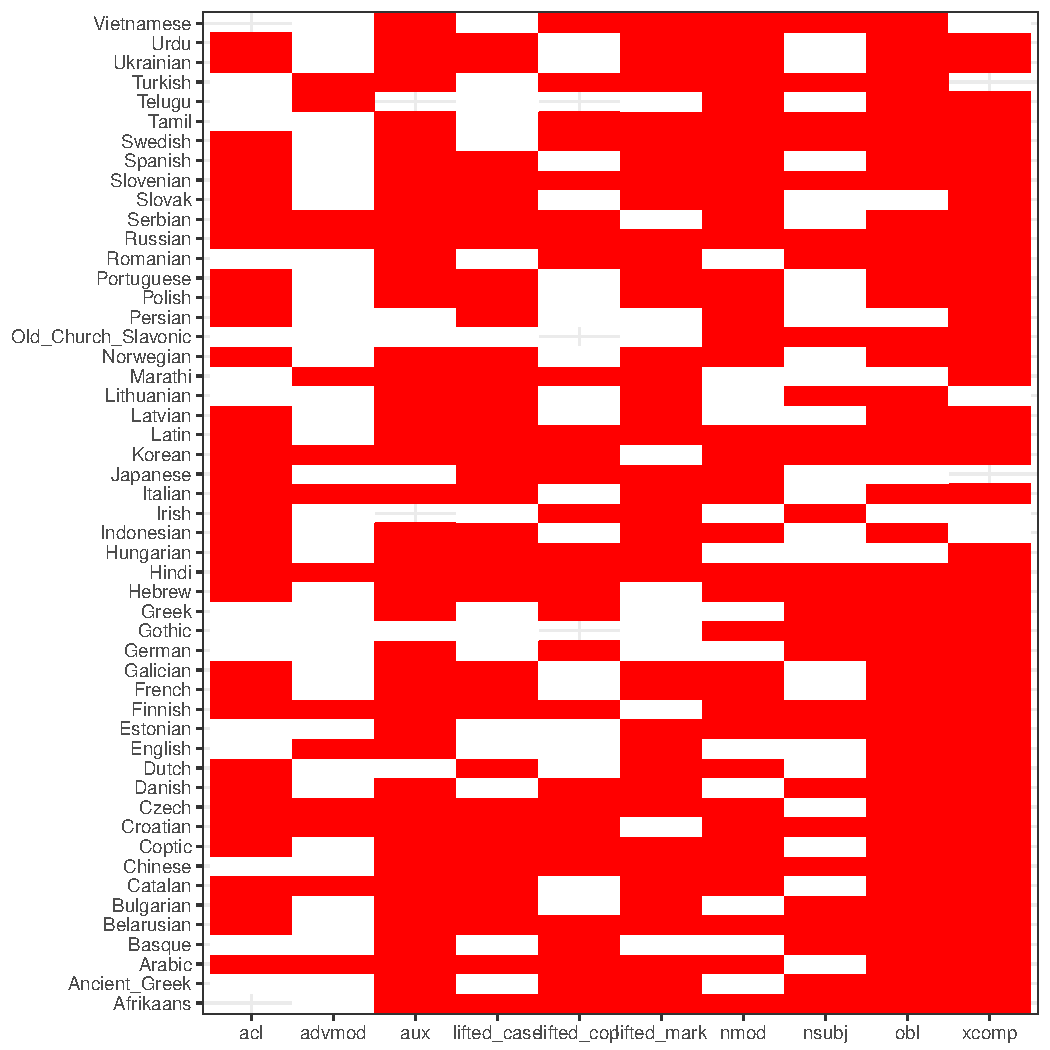
\includegraphics[scale=.25]{../results/correlations/figures/coverage-langmod-best.pdf}
%    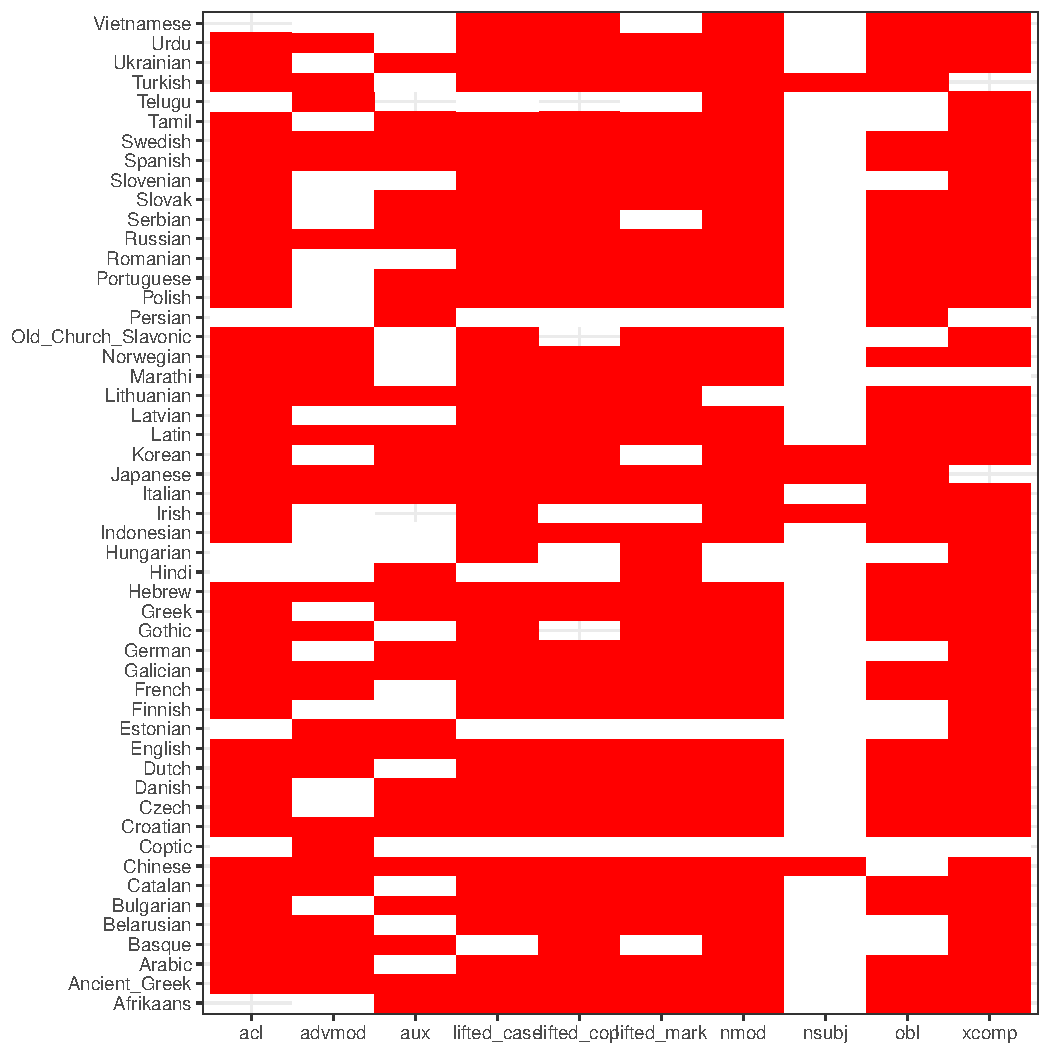
\includegraphics[scale=.25]{../results/correlations/figures/coverage-parse-best.pdf}
%    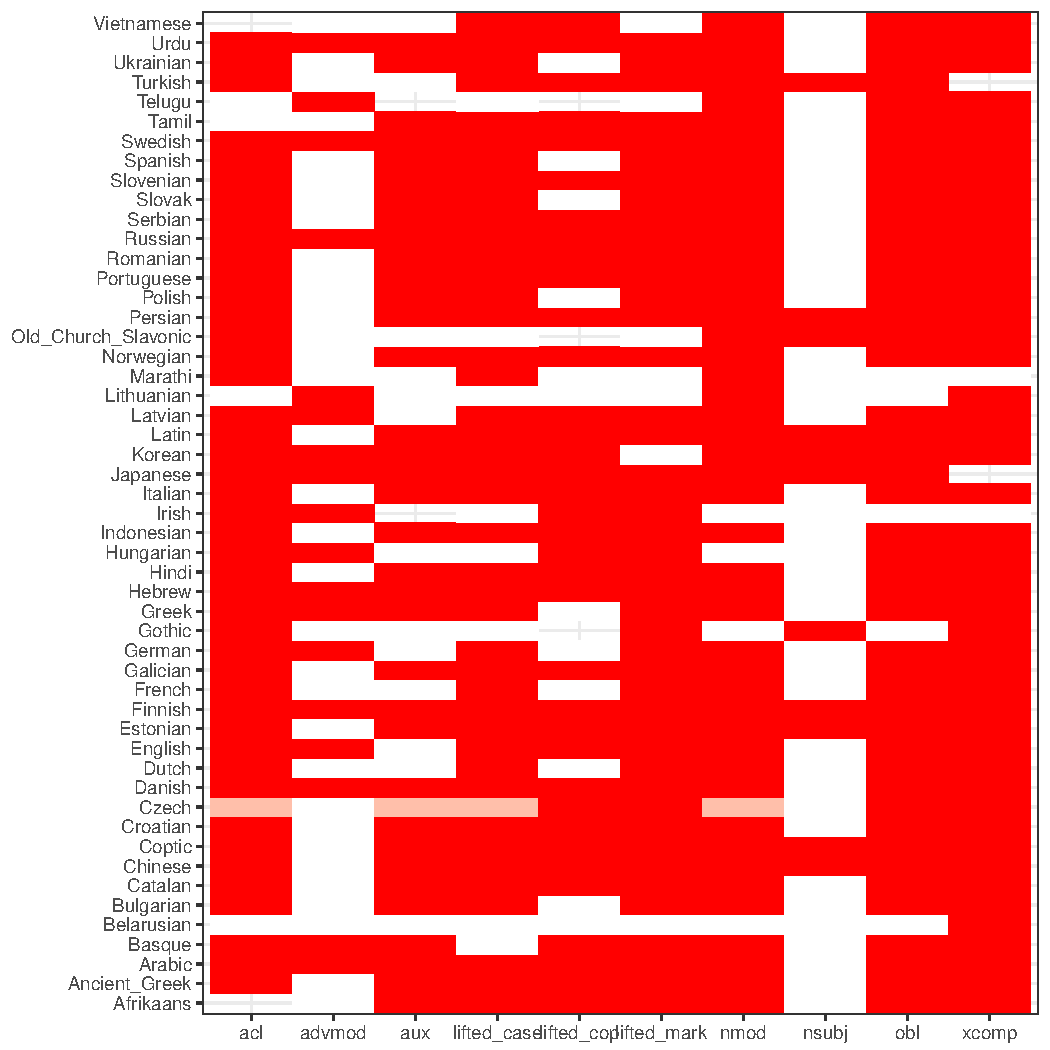
\includegraphics[scale=.25]{../results/correlations/figures/coverage-two-lambda09-best.pdf}
%    
%    
%    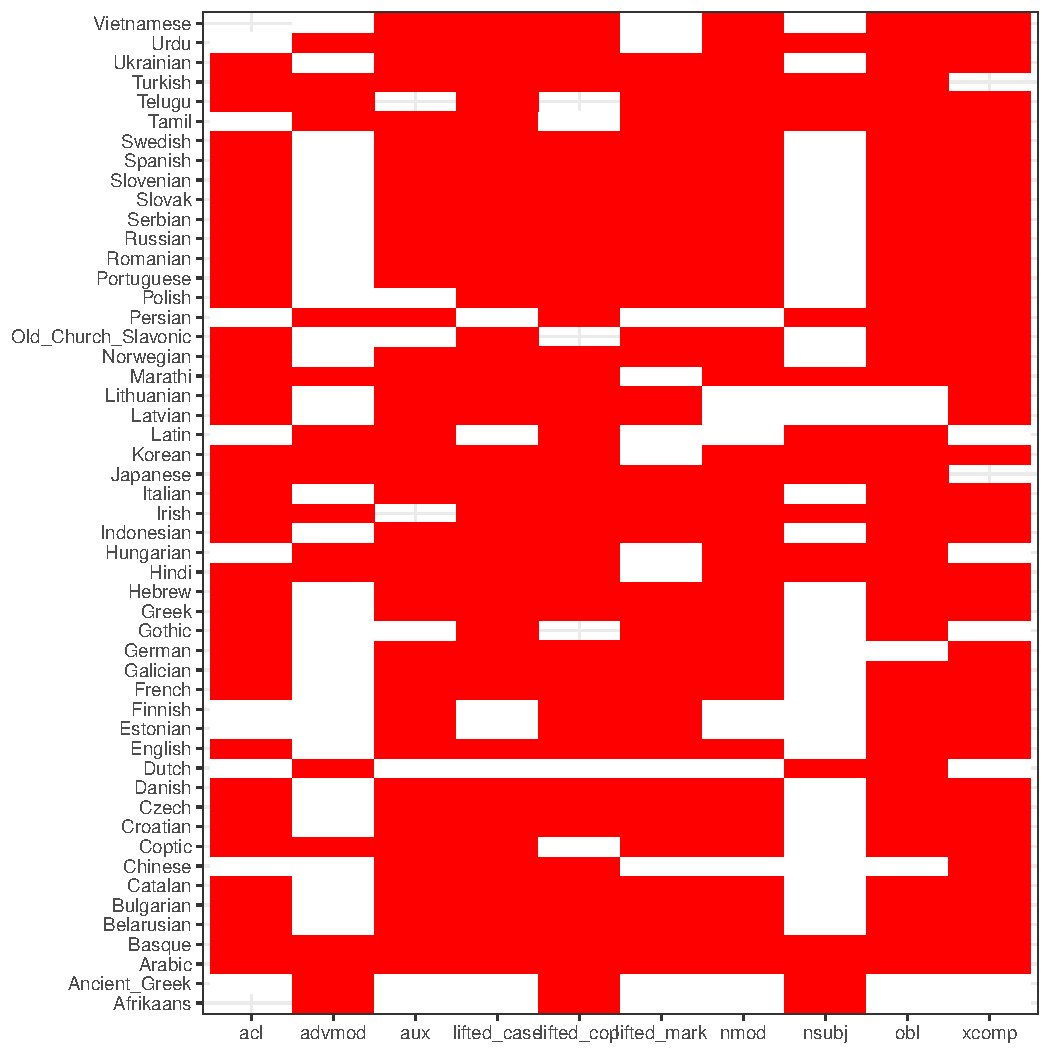
\includegraphics[scale=.25]{../results/correlations/figures/coverage-ground.pdf}
%    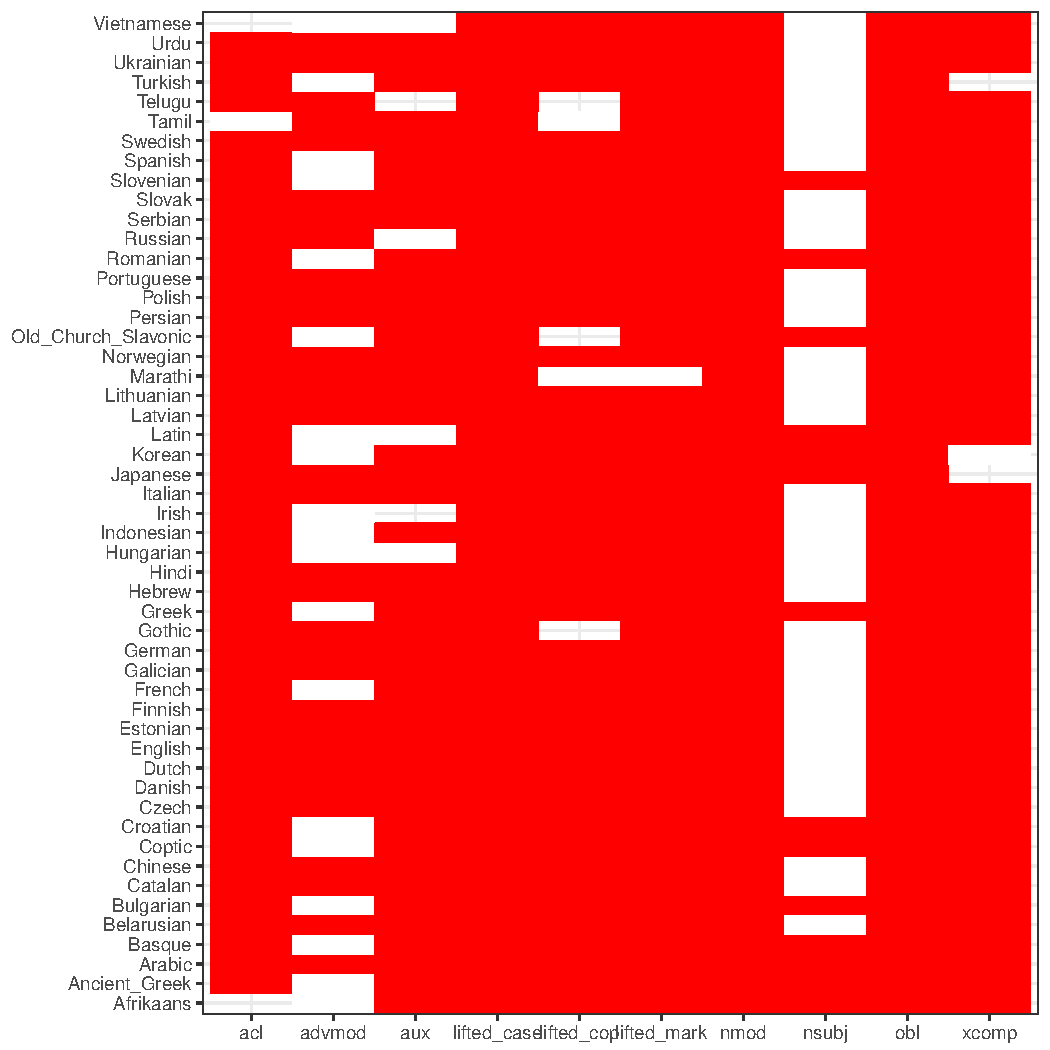
\includegraphics[scale=.25]{../results/correlations/figures/coverage-depl.pdf}
%	\caption{Correlations satisfied by the best word order grammars for predictability, parseability, efficiency, by the UD languages, and by the best grammars for dependency length.}
%    \label{fig:posterior-prevalence}
%\end{figure}



\subsection{Results on all UD Relations}
In this section, we provide the predicted prevalence of correlations between the \emph{obj} dependency and all UD dependency types, along with the expected prevalence according to typological studies.
We also report results for grammars optimized for predictability and parseability individually.


We considered all UD syntactic relations occurring in at least two of the 51 languages.
In Table~\ref{tab:all-predictions-1}, we present the data for the eight correlations discussed in the main paper, and for those other relations for which the typological literature provides data.\footnote{The \emph{aux} syntactic relation in UD has the auxiliary (verb-patterner) as its dependent, and has direction \emph{opposite} to the auxiliary-verb relation \raisebox{.5pt}{\textcircled{\raisebox{-.9pt} {3}}}. Therefore, this relation is \emph{anti-correlated} with the verb-object relation, while \raisebox{.5pt}{\textcircled{\raisebox{-.9pt} {3}}} is \emph{correlated}.  For simplicity, we display this as a corelation in this table.}
Additionally, in Table~\ref{tab:all-predictions-2} we present data for the other UD relations, for which either no typological data is available, or which are not linguistically meaningful.



%We also report results for grammars optimized for Dependency Length Minimization (DLM), which has been argued to be a property of efficient word order, and which we find to be predicted by efficiency optimization (see Section~\ref{sec:DLM}).
%In line with this idea, our results in Table~\ref{tab:all-predictions-1} show that optimizing for DLM makes predictions similar to efficiency optimization.
%These results suggest that it is in part through favoring short dependencies that efficiency predicts word order universals, an idea that has been proposed in prior theoretical studies \citep{hawkins1994performance, hawkins2004efficiency}.
%%Previous theoretical studies arguing for efficiency explanations of word order universals have already suggested that principles akin to DLM explain the Greenberg correlations ; our results provide the first large-scale empirical confirmation of this idea, and show that this can be reduced to efficiency optimization.
%See Section~\ref{sec:DLM} for further discussion.
%



\begin{table*} % TODO figure out away to make this table more aesthetic
	\begin{center}	
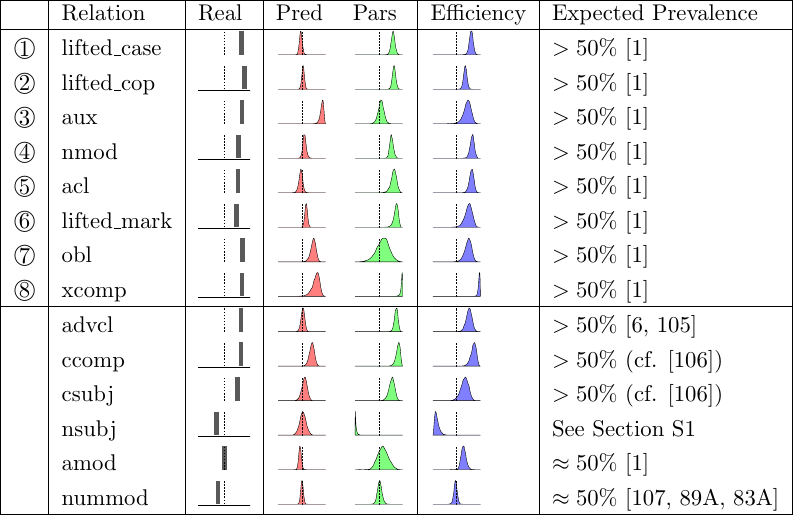
\includegraphics[width=0.8\textwidth]{si-table-perrel-1a-1.png}
\end{center}
\caption{Predictions on UD relations with predictions from the typological literature.
The first section contains the eight correlations discussed in the main paper (See Section~\ref{sec:correlations}); the second section provides other relations for which predictions are available.
The `Real' column provides the prevalence among the 51 languages in the Universal Dependencies data.
We provide posterior prevalences for grammars optimized for Efficiency, and for grammars optimized for Pars(eability) and Pred(ictability) alone, obtained from the Bayesian mixed-effects analysis controlling for languages and language families (as in Table 2 of the main paper).
In the last column, we indicate what prevalence is expected according to the typological literature. 
%We additionally report results obtained when optimizing for Dependency Length Minimization (DLM), a heuristic approximation to efficiency that has been suggested in previous work. See Section~\ref{sec:DLM} for further discussion of DLM and its relation to efficiency. 
}
\label{tab:all-predictions-1}
\end{table*}



%
%%posterior_perRelation_Real_conj.pdf         posterior_perRelation_Real_goeswith.pdf     posterior_perRelation_Real_nummod.pdf       
%%user@user-G751JY:~/grammar-optim/results/correlations$ evince figures/posteriors/posterior_perRelation_Real_csubj.pdf 
%%user@user-G751JY:~/grammar-optim/results/correlations$ 
%
%\begin{table*} % TODO figure out away to make this table more aesthetic
%	\begin{center}	
%\small{
%\begin{tabular}{l|l|l|l|ll|l|l|llllllllllllllllllllllllllll}
%	\hline
%&	Relation & Real & DLM & Pred & Pars & Efficiency & Expected Prevalence  \\ \hline
%% From Dryer	
%\raisebox{.5pt}{\textcircled{\raisebox{-.9pt} {1}}}&	lifted\_case  &  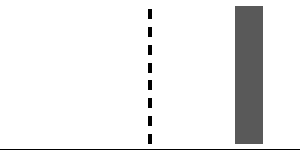
\includegraphics[width=0.06\textwidth]{../results/correlations/figures/posteriors/posterior_perRelation_Real_lifted_case.pdf}   &   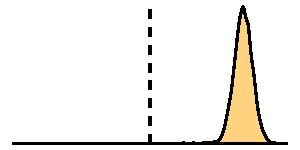
\includegraphics[width=0.06\textwidth]{../results/correlations/figures/posteriors/posterior_perRelation_DependencyLength_lifted_case.pdf}   &   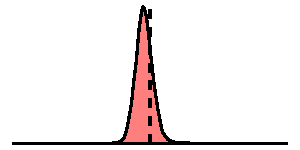
\includegraphics[width=0.06\textwidth]{../results/correlations/figures/posteriors/posterior_perRelation_Predictability_lifted_case.pdf}   &   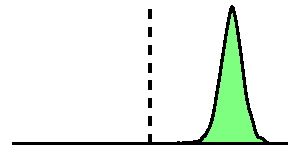
\includegraphics[width=0.06\textwidth]{../results/correlations/figures/posteriors/posterior_perRelation_Parseability_lifted_case.pdf}   &   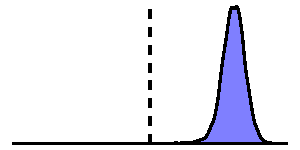
\includegraphics[width=0.06\textwidth]{../results/correlations/figures/posteriors/posterior_perRelation_Efficiency_lifted_case.pdf} & $> 50 \%$ \citep{dryer1992greenbergian}  \\
%\raisebox{.5pt}{\textcircled{\raisebox{-.9pt} {2}}}&	lifted\_cop  &  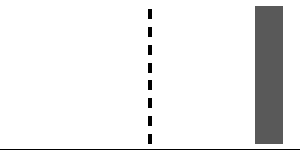
\includegraphics[width=0.06\textwidth]{../results/correlations/figures/posteriors/posterior_perRelation_Real_lifted_cop.pdf}   &   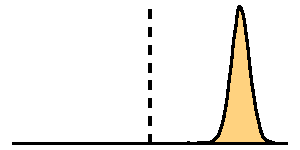
\includegraphics[width=0.06\textwidth]{../results/correlations/figures/posteriors/posterior_perRelation_DependencyLength_lifted_cop.pdf}   &   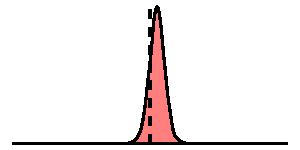
\includegraphics[width=0.06\textwidth]{../results/correlations/figures/posteriors/posterior_perRelation_Predictability_lifted_cop.pdf}   &   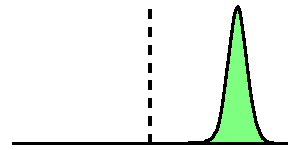
\includegraphics[width=0.06\textwidth]{../results/correlations/figures/posteriors/posterior_perRelation_Parseability_lifted_cop.pdf}   &   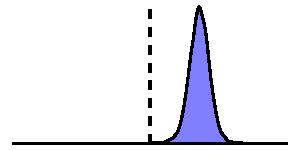
\includegraphics[width=0.06\textwidth]{../results/correlations/figures/posteriors/posterior_perRelation_Efficiency_lifted_cop.pdf} & $> 50 \%$ \citep{dryer1992greenbergian}  \\
%\raisebox{.5pt}{\textcircled{\raisebox{-.9pt} {3}}}&	aux\footnotemark  &  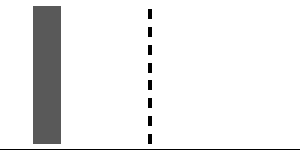
\includegraphics[width=0.06\textwidth]{../results/correlations/figures/posteriors/posterior_perRelation_Real_aux.pdf}   &   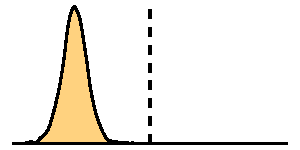
\includegraphics[width=0.06\textwidth]{../results/correlations/figures/posteriors/posterior_perRelation_DependencyLength_aux.pdf}   &   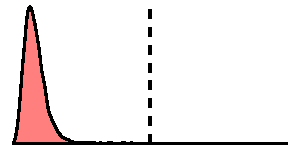
\includegraphics[width=0.06\textwidth]{../results/correlations/figures/posteriors/posterior_perRelation_Predictability_aux.pdf}   &   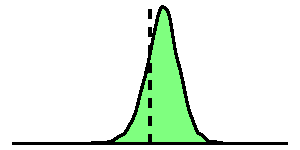
\includegraphics[width=0.06\textwidth]{../results/correlations/figures/posteriors/posterior_perRelation_Parseability_aux.pdf}   &   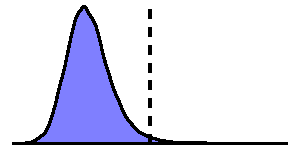
\includegraphics[width=0.06\textwidth]{../results/correlations/figures/posteriors/posterior_perRelation_Efficiency_aux.pdf}  & $<50\%$ \citep{dryer1992greenbergian} \\
%\raisebox{.5pt}{\textcircled{\raisebox{-.9pt} {4}}}&	nmod  &  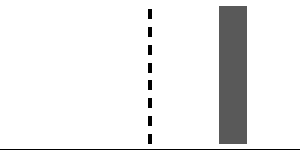
\includegraphics[width=0.06\textwidth]{../results/correlations/figures/posteriors/posterior_perRelation_Real_nmod.pdf}   &   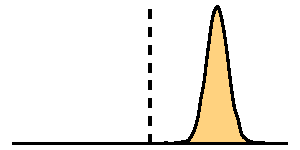
\includegraphics[width=0.06\textwidth]{../results/correlations/figures/posteriors/posterior_perRelation_DependencyLength_nmod.pdf}   &   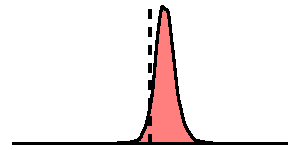
\includegraphics[width=0.06\textwidth]{../results/correlations/figures/posteriors/posterior_perRelation_Predictability_nmod.pdf}   &   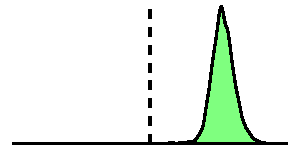
\includegraphics[width=0.06\textwidth]{../results/correlations/figures/posteriors/posterior_perRelation_Parseability_nmod.pdf}   &   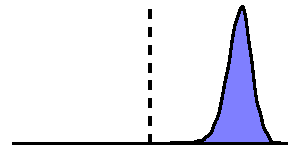
\includegraphics[width=0.06\textwidth]{../results/correlations/figures/posteriors/posterior_perRelation_Efficiency_nmod.pdf}  & $>50\%$ \citep{dryer1992greenbergian} \\
%\raisebox{.5pt}{\textcircled{\raisebox{-.9pt} {5}}}&	acl  &  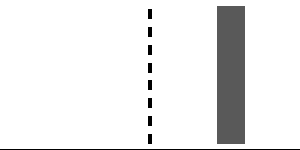
\includegraphics[width=0.06\textwidth]{../results/correlations/figures/posteriors/posterior_perRelation_Real_acl.pdf}   &   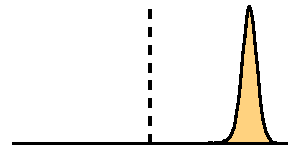
\includegraphics[width=0.06\textwidth]{../results/correlations/figures/posteriors/posterior_perRelation_DependencyLength_acl.pdf}   &   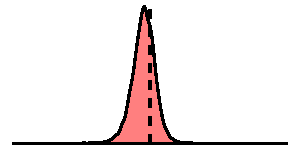
\includegraphics[width=0.06\textwidth]{../results/correlations/figures/posteriors/posterior_perRelation_Predictability_acl.pdf}  &   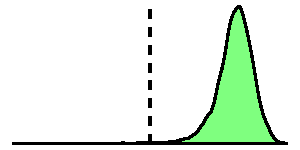
\includegraphics[width=0.06\textwidth]{../results/correlations/figures/posteriors/posterior_perRelation_Parseability_acl.pdf}  &  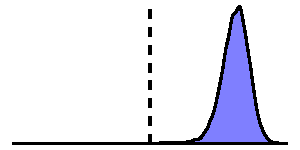
\includegraphics[width=0.06\textwidth]{../results/correlations/figures/posteriors/posterior_perRelation_Efficiency_acl.pdf}   & $>50\%$  \citep{dryer1992greenbergian} \\
%\raisebox{.5pt}{\textcircled{\raisebox{-.9pt} {6}}}&	lifted\_mark  &  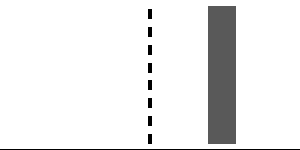
\includegraphics[width=0.06\textwidth]{../results/correlations/figures/posteriors/posterior_perRelation_Real_lifted_mark.pdf}   &   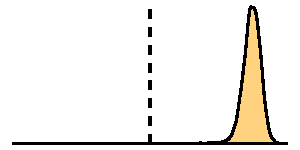
\includegraphics[width=0.06\textwidth]{../results/correlations/figures/posteriors/posterior_perRelation_DependencyLength_lifted_mark.pdf}   &   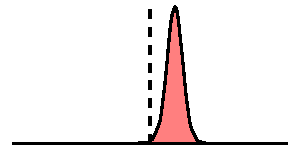
\includegraphics[width=0.06\textwidth]{../results/correlations/figures/posteriors/posterior_perRelation_Predictability_lifted_mark.pdf}   &   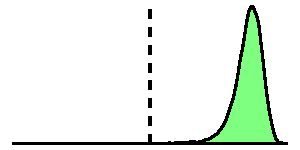
\includegraphics[width=0.06\textwidth]{../results/correlations/figures/posteriors/posterior_perRelation_Parseability_lifted_mark.pdf}   &   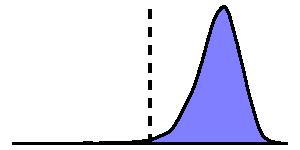
\includegraphics[width=0.06\textwidth]{../results/correlations/figures/posteriors/posterior_perRelation_Efficiency_lifted_mark.pdf} & $> 50 \%$ \citep{dryer1992greenbergian}  \\
%\raisebox{.5pt}{\textcircled{\raisebox{-.9pt} {7}}}&	obl  &  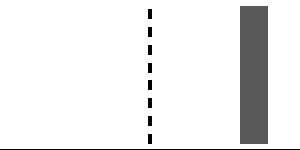
\includegraphics[width=0.06\textwidth]{../results/correlations/figures/posteriors/posterior_perRelation_Real_obl.pdf}   &   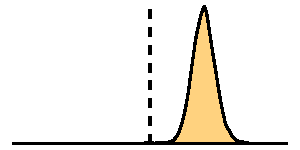
\includegraphics[width=0.06\textwidth]{../results/correlations/figures/posteriors/posterior_perRelation_DependencyLength_obl.pdf}   &   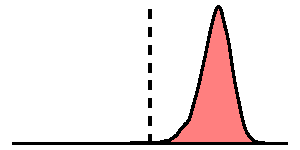
\includegraphics[width=0.06\textwidth]{../results/correlations/figures/posteriors/posterior_perRelation_Predictability_obl.pdf}   &   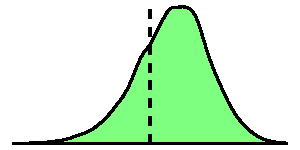
\includegraphics[width=0.06\textwidth]{../results/correlations/figures/posteriors/posterior_perRelation_Parseability_obl.pdf}   &   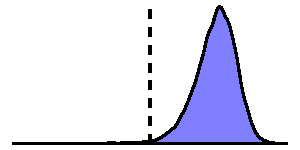
\includegraphics[width=0.06\textwidth]{../results/correlations/figures/posteriors/posterior_perRelation_Efficiency_obl.pdf}  & $>50\%$ \citep{dryer1992greenbergian} \\
%\raisebox{.5pt}{\textcircled{\raisebox{-.9pt} {8}}}&	xcomp  &  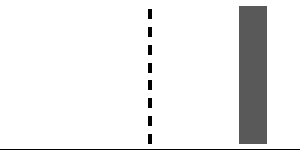
\includegraphics[width=0.06\textwidth]{../results/correlations/figures/posteriors/posterior_perRelation_Real_xcomp.pdf}   &   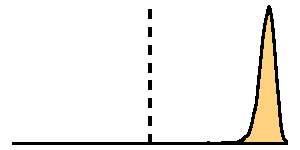
\includegraphics[width=0.06\textwidth]{../results/correlations/figures/posteriors/posterior_perRelation_DependencyLength_xcomp.pdf}   &   \includegraphics[width=0.06\textwidth]{../results/correlations/figures/posteriors/posterior_perRelation_Predictability_xcomp.pdf}   &   \includegraphics[width=0.06\textwidth]{../results/correlations/figures/posteriors/posterior_perRelation_Parseability_xcomp.pdf}   &   \includegraphics[width=0.06\textwidth]{../results/correlations/figures/posteriors/posterior_perRelation_Efficiency_xcomp.pdf}  & $>50\%$ \citep{dryer1992greenbergian} \\
%%\hdashline
%
%\hline
%% Other universals, not in Dryer
%&advcl  &  \includegraphics[width=0.06\textwidth]{../results/correlations/figures/posteriors/posterior_perRelation_Real_advcl.pdf}   &   \includegraphics[width=0.06\textwidth]{../results/correlations/figures/posteriors/posterior_perRelation_DependencyLength_advcl.pdf}   &   \includegraphics[width=0.06\textwidth]{../results/correlations/figures/posteriors/posterior_perRelation_Predictability_advcl.pdf}  &   \includegraphics[width=0.06\textwidth]{../results/correlations/figures/posteriors/posterior_perRelation_Parseability_advcl.pdf}  &  \includegraphics[width=0.06\textwidth]{../results/correlations/figures/posteriors/posterior_perRelation_Efficiency_advcl.pdf}   & $>50\%$ \citep{greenberg1963universals,diessel2001ordering} \\
%&ccomp  &  \includegraphics[width=0.06\textwidth]{../results/correlations/figures/posteriors/posterior_perRelation_Real_ccomp.pdf}   &   \includegraphics[width=0.06\textwidth]{../results/correlations/figures/posteriors/posterior_perRelation_DependencyLength_ccomp.pdf}   &   \includegraphics[width=0.06\textwidth]{../results/correlations/figures/posteriors/posterior_perRelation_Predictability_ccomp.pdf}  &   \includegraphics[width=0.06\textwidth]{../results/correlations/figures/posteriors/posterior_perRelation_Parseability_ccomp.pdf}  &  \includegraphics[width=0.06\textwidth]{../results/correlations/figures/posteriors/posterior_perRelation_Efficiency_ccomp.pdf}   & $>50\%$ (cf. \cite{dryer1980positional}) \\ % TODO According to Dryer 1980, there is a correlation
%&csubj  &  \includegraphics[width=0.06\textwidth]{../results/correlations/figures/posteriors/posterior_perRelation_Real_csubj.pdf}   &   \includegraphics[width=0.06\textwidth]{../results/correlations/figures/posteriors/posterior_perRelation_DependencyLength_csubj.pdf}   &   \includegraphics[width=0.06\textwidth]{../results/correlations/figures/posteriors/posterior_perRelation_Predictability_csubj.pdf}  &   \includegraphics[width=0.06\textwidth]{../results/correlations/figures/posteriors/posterior_perRelation_Parseability_csubj.pdf}  &  \includegraphics[width=0.06\textwidth]{../results/correlations/figures/posteriors/posterior_perRelation_Efficiency_csubj.pdf}   & $>50\%$ (cf. \cite{dryer1980positional}) \\% TODO According to Dryer 1980, there is a correlation
%&nsubj  &  \includegraphics[width=0.06\textwidth]{../results/correlations/figures/posteriors/posterior_perRelation_Real_nsubj.pdf}   &   \includegraphics[width=0.06\textwidth]{../results/correlations/figures/posteriors/posterior_perRelation_DependencyLength_nsubj.pdf}   &   \includegraphics[width=0.06\textwidth]{../results/correlations/figures/posteriors/posterior_perRelation_Predictability_nsubj.pdf}   &   \includegraphics[width=0.06\textwidth]{../results/correlations/figures/posteriors/posterior_perRelation_Parseability_nsubj.pdf}   &   \includegraphics[width=0.06\textwidth]{../results/correlations/figures/posteriors/posterior_perRelation_Efficiency_nsubj.pdf}  & See Section~\ref{sec:correlations} \\
%&amod  &  \includegraphics[width=0.06\textwidth]{../results/correlations/figures/posteriors/posterior_perRelation_Real_amod.pdf}   &   \includegraphics[width=0.06\textwidth]{../results/correlations/figures/posteriors/posterior_perRelation_DependencyLength_amod.pdf}   &   \includegraphics[width=0.06\textwidth]{../results/correlations/figures/posteriors/posterior_perRelation_Predictability_amod.pdf}  &   \includegraphics[width=0.06\textwidth]{../results/correlations/figures/posteriors/posterior_perRelation_Parseability_amod.pdf}  &  \includegraphics[width=0.06\textwidth]{../results/correlations/figures/posteriors/posterior_perRelation_Efficiency_amod.pdf}   &  $\approx 50\%$ \citep{dryer1992greenbergian} \\
%&nummod  &  \includegraphics[width=0.06\textwidth]{../results/correlations/figures/posteriors/posterior_perRelation_Real_nummod.pdf}   &   \includegraphics[width=0.06\textwidth]{../results/correlations/figures/posteriors/posterior_perRelation_DependencyLength_nummod.pdf}   &   \includegraphics[width=0.06\textwidth]{../results/correlations/figures/posteriors/posterior_perRelation_Predictability_nummod.pdf}  &   \includegraphics[width=0.06\textwidth]{../results/correlations/figures/posteriors/posterior_perRelation_Parseability_nummod.pdf}  &  \includegraphics[width=0.06\textwidth]{../results/correlations/figures/posteriors/posterior_perRelation_Efficiency_nummod.pdf}   &$\approx 50\%$ \citep[][89A, 83A]{wals} \\ 
% \hline
%%comp. &
%%\multirow{3}{*}{NP}&
%%	AP &
%\end{tabular}
%}
%
%\end{center}
%\caption{Predictions on UD relations with predictions from the typological literature. The first section contains the eight correlations discussed in the main paper (See Section~\ref{sec:correlations}); the second section provides other relations for which predictions are available. In the last column, we indicate what direction would be expected typologically.}
%\label{tab:all-predictions-1}
%\end{table*}
%





%\footnotetext{Note that we report an \emph{anti-correlation}. The \emph{aux} syntactic relation in UD has the auxiliary (verb-patterner) as its dependent, and has direction \emph{opposite} to the auxiliary-verb relation \raisebox{.5pt}{\textcircled{\raisebox{-.9pt} {3}}}. Therefore, this relation is \emph{anti-correlated} with the verb-object relation, while \raisebox{.5pt}{\textcircled{\raisebox{-.9pt} {3}}} is \emph{correlated}.  }





\begin{table*} % TODO figure out away to make this table more aesthetic
	\begin{center}	
\includegraphics[width=0.7\textwidth]{si-table-perrel-2a-1.png}  
\end{center}
\caption{Predictions on UD relations for which no predictions are available in the typological literature.  ``Uninterpretable'' UD relations are those which collapse so many different linguistic relationships that they are not linguistically meaningful. ``UD artifact'' relations are those whose order is determined strictly by UD parsing standards, such that their order is not linguistically meaningful: these include dependencies such as the connection between two parts of a word that have been separated by whitespace inserted as a typo (\emph{goeswith}).
We provide results for grammars optimized for Efficiency, and for grammars optimized for Pars(eability) and Pred(ictability) alone.
}
\label{tab:all-predictions-2}
\end{table*}





%
%\begin{table*} % TODO figure out away to make this table more aesthetic
%	\begin{center}	
%\small{
%\begin{tabular}{|l|l|l|ll|l|l|llllllllllllllllllllllllllll}
%	\hline
%	Relation & Real & DLM & Pred & Pars & Efficiency & Expected Prevalence  \\ \hline
%\hline
%appos  &  \includegraphics[width=0.06\textwidth]{../results/correlations/figures/posteriors/posterior_perRelation_Real_appos.pdf}   &   \includegraphics[width=0.06\textwidth]{../results/correlations/figures/posteriors/posterior_perRelation_DependencyLength_appos.pdf}   &   \includegraphics[width=0.06\textwidth]{../results/correlations/figures/posteriors/posterior_perRelation_Predictability_appos.pdf}  &   \includegraphics[width=0.06\textwidth]{../results/correlations/figures/posteriors/posterior_perRelation_Parseability_appos.pdf}  &  \includegraphics[width=0.06\textwidth]{../results/correlations/figures/posteriors/posterior_perRelation_Efficiency_appos.pdf}   &                                               Unknown \\           
%lifted\_cc  &  \includegraphics[width=0.06\textwidth]{../results/correlations/figures/posteriors/posterior_perRelation_Real_lifted_cc.pdf}   &   \includegraphics[width=0.06\textwidth]{../results/correlations/figures/posteriors/posterior_perRelation_DependencyLength_lifted_cc.pdf}   &   \includegraphics[width=0.06\textwidth]{../results/correlations/figures/posteriors/posterior_perRelation_Predictability_lifted_cc.pdf}  &   \includegraphics[width=0.06\textwidth]{../results/correlations/figures/posteriors/posterior_perRelation_Parseability_lifted_cc.pdf}  &  \includegraphics[width=0.06\textwidth]{../results/correlations/figures/posteriors/posterior_perRelation_Efficiency_lifted_cc.pdf}   &                  Unknown \\          
%expl  &  \includegraphics[width=0.06\textwidth]{../results/correlations/figures/posteriors/posterior_perRelation_Real_expl.pdf}   &   \includegraphics[width=0.06\textwidth]{../results/correlations/figures/posteriors/posterior_perRelation_DependencyLength_expl.pdf}   &   \includegraphics[width=0.06\textwidth]{../results/correlations/figures/posteriors/posterior_perRelation_Predictability_expl.pdf}  &   \includegraphics[width=0.06\textwidth]{../results/correlations/figures/posteriors/posterior_perRelation_Parseability_expl.pdf}  &  \includegraphics[width=0.06\textwidth]{../results/correlations/figures/posteriors/posterior_perRelation_Efficiency_expl.pdf}   &                                                        Unknown \\         
%iobj  &  \includegraphics[width=0.06\textwidth]{../results/correlations/figures/posteriors/posterior_perRelation_Real_iobj.pdf}   &   \includegraphics[width=0.06\textwidth]{../results/correlations/figures/posteriors/posterior_perRelation_DependencyLength_iobj.pdf}   &   \includegraphics[width=0.06\textwidth]{../results/correlations/figures/posteriors/posterior_perRelation_Predictability_iobj.pdf}  &   \includegraphics[width=0.06\textwidth]{../results/correlations/figures/posteriors/posterior_perRelation_Parseability_iobj.pdf}  &  \includegraphics[width=0.06\textwidth]{../results/correlations/figures/posteriors/posterior_perRelation_Efficiency_iobj.pdf}   &                                                        Unknown \\     
%vocative  &  \includegraphics[width=0.06\textwidth]{../results/correlations/figures/posteriors/posterior_perRelation_Real_vocative.pdf}   &   \includegraphics[width=0.06\textwidth]{../results/correlations/figures/posteriors/posterior_perRelation_DependencyLength_vocative.pdf}   &   \includegraphics[width=0.06\textwidth]{../results/correlations/figures/posteriors/posterior_perRelation_Predictability_vocative.pdf}  &   \includegraphics[width=0.06\textwidth]{../results/correlations/figures/posteriors/posterior_perRelation_Parseability_vocative.pdf}  &  \includegraphics[width=0.06\textwidth]{../results/correlations/figures/posteriors/posterior_perRelation_Efficiency_vocative.pdf}   &                            Unknown \\ 
%
%\hline
%% Uninterpretable
%compound  &  \includegraphics[width=0.06\textwidth]{../results/correlations/figures/posteriors/posterior_perRelation_Real_compound.pdf}   &   \includegraphics[width=0.06\textwidth]{../results/correlations/figures/posteriors/posterior_perRelation_DependencyLength_compound.pdf}   &   \includegraphics[width=0.06\textwidth]{../results/correlations/figures/posteriors/posterior_perRelation_Predictability_compound.pdf}  &   \includegraphics[width=0.06\textwidth]{../results/correlations/figures/posteriors/posterior_perRelation_Parseability_compound.pdf}  &  \includegraphics[width=0.06\textwidth]{../results/correlations/figures/posteriors/posterior_perRelation_Efficiency_compound.pdf}   &                       Uninterpretable \\        
%det  &  \includegraphics[width=0.06\textwidth]{../results/correlations/figures/posteriors/posterior_perRelation_Real_det.pdf}   &   \includegraphics[width=0.06\textwidth]{../results/correlations/figures/posteriors/posterior_perRelation_DependencyLength_det.pdf}   &   \includegraphics[width=0.06\textwidth]{../results/correlations/figures/posteriors/posterior_perRelation_Predictability_det.pdf}  &   \includegraphics[width=0.06\textwidth]{../results/correlations/figures/posteriors/posterior_perRelation_Parseability_det.pdf}  &  \includegraphics[width=0.06\textwidth]{../results/correlations/figures/posteriors/posterior_perRelation_Efficiency_det.pdf}   &                                                    Uninterpretable \\        
%dislocated  &  \includegraphics[width=0.06\textwidth]{../results/correlations/figures/posteriors/posterior_perRelation_Real_dislocated.pdf}   &   \includegraphics[width=0.06\textwidth]{../results/correlations/figures/posteriors/posterior_perRelation_DependencyLength_dislocated.pdf}   &   \includegraphics[width=0.06\textwidth]{../results/correlations/figures/posteriors/posterior_perRelation_Predictability_dislocated.pdf}  &   \includegraphics[width=0.06\textwidth]{../results/correlations/figures/posteriors/posterior_perRelation_Parseability_dislocated.pdf}  &  \includegraphics[width=0.06\textwidth]{../results/correlations/figures/posteriors/posterior_perRelation_Efficiency_dislocated.pdf}   &             Uninterpretable \\               
%dep  &  \includegraphics[width=0.06\textwidth]{../results/correlations/figures/posteriors/posterior_perRelation_Real_dep.pdf}   &   \includegraphics[width=0.06\textwidth]{../results/correlations/figures/posteriors/posterior_perRelation_DependencyLength_dep.pdf}   &   \includegraphics[width=0.06\textwidth]{../results/correlations/figures/posteriors/posterior_perRelation_Predictability_dep.pdf}  &   \includegraphics[width=0.06\textwidth]{../results/correlations/figures/posteriors/posterior_perRelation_Parseability_dep.pdf}  &  \includegraphics[width=0.06\textwidth]{../results/correlations/figures/posteriors/posterior_perRelation_Efficiency_dep.pdf}   &                                                 Uninterpretable \\
%advmod  &  \includegraphics[width=0.06\textwidth]{../results/correlations/figures/posteriors/posterior_perRelation_Real_advmod.pdf}   &   \includegraphics[width=0.06\textwidth]{../results/correlations/figures/posteriors/posterior_perRelation_DependencyLength_advmod.pdf}   &   \includegraphics[width=0.06\textwidth]{../results/correlations/figures/posteriors/posterior_perRelation_Predictability_advmod.pdf}  &   \includegraphics[width=0.06\textwidth]{../results/correlations/figures/posteriors/posterior_perRelation_Parseability_advmod.pdf}  &  \includegraphics[width=0.06\textwidth]{../results/correlations/figures/posteriors/posterior_perRelation_Efficiency_advmod.pdf}   &                                         Uninterpretable \\ 
%
%\hline
%% UD artifacts
%conj  &  \includegraphics[width=0.06\textwidth]{../results/correlations/figures/posteriors/posterior_perRelation_Real_conj.pdf}   &   \includegraphics[width=0.06\textwidth]{../results/correlations/figures/posteriors/posterior_perRelation_DependencyLength_conj.pdf}   &   \includegraphics[width=0.06\textwidth]{../results/correlations/figures/posteriors/posterior_perRelation_Predictability_conj.pdf}  &   \includegraphics[width=0.06\textwidth]{../results/correlations/figures/posteriors/posterior_perRelation_Parseability_conj.pdf}  &  \includegraphics[width=0.06\textwidth]{../results/correlations/figures/posteriors/posterior_perRelation_Efficiency_conj.pdf}   &                                                      UD Artifact \\
%discourse  &  \includegraphics[width=0.06\textwidth]{../results/correlations/figures/posteriors/posterior_perRelation_Real_discourse.pdf}   &   \includegraphics[width=0.06\textwidth]{../results/correlations/figures/posteriors/posterior_perRelation_DependencyLength_discourse.pdf}   &   \includegraphics[width=0.06\textwidth]{../results/correlations/figures/posteriors/posterior_perRelation_Predictability_discourse.pdf}  &   \includegraphics[width=0.06\textwidth]{../results/correlations/figures/posteriors/posterior_perRelation_Parseability_discourse.pdf}  &  \includegraphics[width=0.06\textwidth]{../results/correlations/figures/posteriors/posterior_perRelation_Efficiency_discourse.pdf}   &                 UD Artifact \\ 
%fixed  &  \includegraphics[width=0.06\textwidth]{../results/correlations/figures/posteriors/posterior_perRelation_Real_fixed.pdf}   &   \includegraphics[width=0.06\textwidth]{../results/correlations/figures/posteriors/posterior_perRelation_DependencyLength_fixed.pdf}   &   \includegraphics[width=0.06\textwidth]{../results/correlations/figures/posteriors/posterior_perRelation_Predictability_fixed.pdf}  &   \includegraphics[width=0.06\textwidth]{../results/correlations/figures/posteriors/posterior_perRelation_Parseability_fixed.pdf}  &  \includegraphics[width=0.06\textwidth]{../results/correlations/figures/posteriors/posterior_perRelation_Efficiency_fixed.pdf}   &                                             UD Artifact \\ 
%flat  &  \includegraphics[width=0.06\textwidth]{../results/correlations/figures/posteriors/posterior_perRelation_Real_flat.pdf}   &   \includegraphics[width=0.06\textwidth]{../results/correlations/figures/posteriors/posterior_perRelation_DependencyLength_flat.pdf}   &   \includegraphics[width=0.06\textwidth]{../results/correlations/figures/posteriors/posterior_perRelation_Predictability_flat.pdf}  &   \includegraphics[width=0.06\textwidth]{../results/correlations/figures/posteriors/posterior_perRelation_Parseability_flat.pdf}  &  \includegraphics[width=0.06\textwidth]{../results/correlations/figures/posteriors/posterior_perRelation_Efficiency_flat.pdf}   &                                                      UD Artifact \\
%goeswith  &  \includegraphics[width=0.06\textwidth]{../results/correlations/figures/posteriors/posterior_perRelation_Real_goeswith.pdf}   &   \includegraphics[width=0.06\textwidth]{../results/correlations/figures/posteriors/posterior_perRelation_DependencyLength_goeswith.pdf}   &   \includegraphics[width=0.06\textwidth]{../results/correlations/figures/posteriors/posterior_perRelation_Predictability_goeswith.pdf}  &   \includegraphics[width=0.06\textwidth]{../results/correlations/figures/posteriors/posterior_perRelation_Parseability_goeswith.pdf}  &  \includegraphics[width=0.06\textwidth]{../results/correlations/figures/posteriors/posterior_perRelation_Efficiency_goeswith.pdf}   &                          UD Artifact \\
%list  &  \includegraphics[width=0.06\textwidth]{../results/correlations/figures/posteriors/posterior_perRelation_Real_list.pdf}   &   \includegraphics[width=0.06\textwidth]{../results/correlations/figures/posteriors/posterior_perRelation_DependencyLength_list.pdf}   &   \includegraphics[width=0.06\textwidth]{../results/correlations/figures/posteriors/posterior_perRelation_Predictability_list.pdf}  &   \includegraphics[width=0.06\textwidth]{../results/correlations/figures/posteriors/posterior_perRelation_Parseability_list.pdf}  &  \includegraphics[width=0.06\textwidth]{../results/correlations/figures/posteriors/posterior_perRelation_Efficiency_list.pdf}   &                                                      UD Artifact \\
%orphan  &  \includegraphics[width=0.06\textwidth]{../results/correlations/figures/posteriors/posterior_perRelation_Real_orphan.pdf}   &   \includegraphics[width=0.06\textwidth]{../results/correlations/figures/posteriors/posterior_perRelation_DependencyLength_orphan.pdf}   &   \includegraphics[width=0.06\textwidth]{../results/correlations/figures/posteriors/posterior_perRelation_Predictability_orphan.pdf}  &   \includegraphics[width=0.06\textwidth]{../results/correlations/figures/posteriors/posterior_perRelation_Parseability_orphan.pdf}  &  \includegraphics[width=0.06\textwidth]{../results/correlations/figures/posteriors/posterior_perRelation_Efficiency_orphan.pdf}   & UD Artifact \\                                        
%parataxis  &  \includegraphics[width=0.06\textwidth]{../results/correlations/figures/posteriors/posterior_perRelation_Real_parataxis.pdf}   &   \includegraphics[width=0.06\textwidth]{../results/correlations/figures/posteriors/posterior_perRelation_DependencyLength_parataxis.pdf}   &   \includegraphics[width=0.06\textwidth]{../results/correlations/figures/posteriors/posterior_perRelation_Predictability_parataxis.pdf}  &   \includegraphics[width=0.06\textwidth]{../results/correlations/figures/posteriors/posterior_perRelation_Parseability_parataxis.pdf}  &  \includegraphics[width=0.06\textwidth]{../results/correlations/figures/posteriors/posterior_perRelation_Efficiency_parataxis.pdf}   &                 UD Artifact \\   
%reparandum  &  \includegraphics[width=0.06\textwidth]{../results/correlations/figures/posteriors/posterior_perRelation_Real_reparandum.pdf}   &   \includegraphics[width=0.06\textwidth]{../results/correlations/figures/posteriors/posterior_perRelation_DependencyLength_reparandum.pdf}   &   \includegraphics[width=0.06\textwidth]{../results/correlations/figures/posteriors/posterior_perRelation_Predictability_reparandum.pdf}  &   \includegraphics[width=0.06\textwidth]{../results/correlations/figures/posteriors/posterior_perRelation_Parseability_reparandum.pdf}  &  \includegraphics[width=0.06\textwidth]{../results/correlations/figures/posteriors/posterior_perRelation_Efficiency_reparandum.pdf}   &                UD Artifact \\          
%
% \hline
%%comp. &
%%\multirow{3}{*}{NP}&
%%	AP &
%\end{tabular}
%}
%
%\end{center}
%\caption{Predictions on UD relations for which no predictions are available in the typological literature.  ``Uninterpretable'' UD relations are those which collapse so many different linguistic relationships that they are not linguistically meaningful. ``UD artifact'' relations are those whose order is determined strictly by UD parsing standards, such that their order is not linguistically meaningful: these include dependencies such as the connection between two parts of a word that have been separated by whitespace inserted as a typo (\emph{goeswith}).}
%\label{tab:all-predictions-2}
%\end{table*}
%
%






\subsection{Previous Experiments}\label{sec:previous-exps}
In Table~\ref{table:corr-resu-previous} we report the results of our two previous, preregistered, simulations\footnote{\url{http://aspredicted.org/blind.php?x=8gp2bt}, \url{https://aspredicted.org/blind.php?x=bg35x7}. For the results of the Locality simulations described in the first preregistration, see the Dependency Length Minimization results in Table~\ref{tab:all-predictions-1b}, with discussion in Section~\ref{sec:DLM}.} together with results from the main experiment.
These experiments all had the same setup described in Section~\ref{sec:neural-architectures}, which was fixed before starting simulations; differences are that (1) one simulation places fully equal weight on parseability and predictability ($\lambda=1.0$), and (2) the final experiment uses three random seeds per grammar.
Results across all three experiments agree; jointly optimizing grammars for parseability and predictability produces all eight correlations.


\begin{table}[hbt!]

	\begin{center}
\includegraphics[width=0.4\textwidth]{si-table-perrel-3-1.png}  
\end{center}

	\begin{center}
\begin{tabular}{cccc}
$\lambda=0.0$ & $\lambda=0.9$ & $\lambda=0.9$ & $\lambda=1.0$ \\
	\includegraphics[width=0.15\textwidth]{../results/correlations/figures/posterior-satisfied-universals-parseability.pdf}&
	\includegraphics[width=0.15\textwidth]{../results/correlations/figures/posterior-satisfied-universals-together-large-prior-efficiency09.pdf}&
	\includegraphics[width=0.15\textwidth]{../results/correlations/figures/posterior-satisfied-universals-efficiency-large.pdf}&
	\includegraphics[width=0.15\textwidth]{../results/correlations/figures/posterior-satisfied-universals-together-large-prior-efficiency10.pdf}
\end{tabular}
	\end{center}
	\caption{Results from optimization experiments for different values of $\lambda$, including our two previous preregistered experiments (Section~\ref{sec:previous-exps}). For comparison, we also show results for $\lambda=0$, corresponding to optimizing for parseability only (same results as reported in Tables (\ref{tab:all-predictions-1}-\ref{tab:all-predictions-2})). For $\lambda=0.9$, we report results from one preliminary preregistered experiment (left) and the final experiment (right). For $\lambda=1.0$, we report the other preliminary preregistered experiment.
Giving similar weight to parseability and predictability -- that is, $\lambda$ close to $1$ -- results in more accurate word order predictions than choosing a small value of $\lambda$ such as $\lambda=0.0$. Note that $\lambda$ cannot take values smaller than zero, or greater than one, see Section \ref{sec:lambda}.
}\label{table:corr-resu-previous}
\end{table}



%\section{Joint optimization of grammar, parser, and language model parameters}
\section{Creating Optimized Grammars}

In this section, we describe the method we employ for creating grammars that are optimized for efficiency, and how we extract grammars describing the actual ordering rules of languages.
%Our method will be applicable more generally to the task of optimizing grammars for a broad class of objective functions.
We carry out grammar optimization in an extended space of grammars that interpolates continuously between different grammars (Section~\ref{sec:diff-gramm}).
More specifically, we include probabilistic relaxations of grammars, which describe probability distributions over different ways of ordering a syntactic structure into a sentence.
This makes efficiency a \emph{differentiable} function of the grammar parameters, and enables efficient optimization with stochastic gradient descent, as we describe in Section~\ref{sec:optim-eff}.

This method addresses a major challenge noted in previous work optimizing grammars, namely that the predictability (and parseability) of an individual sentence depends on the entire distribution of the language.
Previously, \citet{gildea2015human} optimized grammars for dependency length and trigram surprisal using a simple hill-climbing method on the grammar parameters, which required reestimating the trigram surprisal model in every iteration.
Such a method would be computationally prohibitive for efficiency optimization, as it would require reestimating the neural network models after every change to the grammar, which would amount to reestimating them hundreds or thousands of times per grammar.
Our method, by allowing for the use of stochastic gradient descent, addresses this challenge, as we describe in Section~\ref{sec:optim-eff}.


\subsection{Differentiable Ordering Grammars}\label{sec:diff-gramm}

We extended the parameter space of grammars by continuously interpolating between grammars, making efficiency a \emph{differentiable} function of grammar parameters.
The parameters of such a \key{differentiable word order grammar} are as follows. 
For each dependency label type $\tau$, we have (1) a \key{Direction Parameter} $a_\tau \in [0,1]$, and (2) a \key{Distance Parameter} $b_\tau \in \mathbb{R}$. 
Each dependent is ordered on the left of its head with probability $a_\tau$ and to the right with probability $1-a_\tau$. 
Then for each set of co-dependents $\{s_1, \dots , s_n\}$ placed on one side of a head, their order outward from the head is determined by iteratively sampling from the distribution $\operatorname{softmax}(b_{\tau_1}, \dots, b_{\tau_n})$ (\cite{goodfellow2016deep}, p. 184) without replacement. 

If $a_\tau \in \{0, 1\}$, and the distances between values of $b_\tau$ (for different $\tau$) become very large, such a differentiable grammar becomes deterministic, assigning almost full probability to exactly one ordering for each syntactic structure.
In this case, the grammar can be converted into an equivalent grammar of the form described in Materials and Methods, by extracting a single parameter in $[-1, 1]$ for each relation $\tau$.

We provide an example in Figure~\ref{fig:grammar-sample}, illustrating grammar parameters for the relations in Figure 3 of the main paper.
Note that the grammatical formalism simplifies some aspects of the word order regularities of natural languages.
For instance, it does not represent cases where ordering varies between main and embedded clauses, as it does not condition ordering decisions on the larger context.
%Our method extracts the most frequent ordering and applies it throughout all 
More complex and powerful ordering grammar models have been proposed \cite{futrell2015experiments, wang2016galactic}; however, they have similar limitations, and for our purposes, the model adopted here has the advantage of being simple and interpretable.
%There currently is no grammatical formalism that is at the same time capable of representing the full range of word order regularities that are found, 
%\cite{futrell2015experiments}



\begin{figure}
	\begin{center}
\begin{tabular}{l||l|ll||l|lllll}
	& \multicolumn{3}{c||}{English}    &  \multicolumn{3}{c}{Japanese}  \\ 
	Relation                     &  Par.   & $a_\tau$ & $b_\tau$            & Par.   & $a_\tau$ & $b_\tau$     \\ \hline \hline
	object (\textit{obj})        &  $0.1$   &   $0.04$   & $-1.46$            & $-0.1$  & $0.99$ & $-0.7$2 \\
	oblique (\textit{obl})       &  $0.3$   &   $0.13$     & $1.25$             & $-0.3$  & $0.99$ & $0.73$ \\
	case (\textit{lifted\_case}) &  $0.2$   &   $0.07$       &   $-0.89$         & $-0.2$  &  $0.92$ & $0.02$  \\
\end{tabular}
	\end{center}
	\caption{Sample Coefficients from grammars extracted from the real English and Japanese orderings (Section~\ref{sec:extract-grammars}), for the relations occurring in Figure 3 (Main Paper). We show parameters in $[-1,1]$ for deterministic word order grammars as described in \emph{Materials and Methods}, and the coefficients ($a_\tau, b_\tau$) for corresponding differentiable ordering grammars. For the deterministic grammars (`Par.'), positive coefficients indicate that the dependent will be placed after the head. For the differentiable grammars, $a_\tau > 0.5$ indicates predominance of ordering of dependents before heads, and larger $b_\tau$ indicates greater distance between head and dependent.}\label{fig:grammar-sample}
\end{figure}


\subsection{Extracting Grammars from Datasets}\label{sec:extract-grammars}
We extract grammars for each actual language by fitting a differentiable ordering grammar maximizing the likelihood of the observed orderings.
To prevent overfitting, we regularize each $a_\tau$, $b_\tau$ with a simple Bayesian prior $logit(a_\tau) \sim \mathcal{N}(0,1)$, $b_\tau \sim \mathcal{N}(0,1)$.
We implemented this regularized optimization as mean-field ELBO variational inference in Pyro~\cite{bingham2018pyro}.
We then extract the posterior means for each parameter $a_\tau, b_\tau$, and convert the resulting differentiable grammar into an ordinary ordering grammar.




We validated the extracted grammars by comparing the dominant orders of six syntactic relations that are also annotated in the World Atlas of Linguistic Structures (WALS, \cite{haspelmath2005world}).
Among the eight Greenbergian correlations that we were able to test, five are annotated in WALS: adpositions, complementizers, relative clauses, genitives, and oblique PPs.
In Table~\ref{tab:grammars-wals}, we compare our grammars with WALS on these five relations, and the verb-object relation.
WALS has data for 74\% of the entries\footnote{Serbian and Croatian are listed as a single language Serbian-Croatian in WALS. In the table, we compare those with the grammar we extracted for Croatian, noting that it fully agrees with the Serbian grammar.}, and lists a dominant order for 91\% of these.
The grammars we extracted from the corpora agree with WALS in 96~\%  of these cases.




\begin{table}
\small{
\begin{center}
\begin{tabular}{l||ll|ll|ll|ll|ll|ll|llllll}
%	   for(dep in c("obj", "lifted_mark", "acl", "nmod", "obl")) {
		   Language 
		   &	\multicolumn{2}{c|}{Objects} 
		   &	\multicolumn{2}{c|}{Adpositions} 
		   &	\multicolumn{2}{c|}{Compl.} 
		   &	\multicolumn{2}{c|}{Rel.Cl.} 
		   &	\multicolumn{2}{c|}{Genitive} 
		   &	\multicolumn{2}{c|}{PP}  \\ \hline\hline
	Afrikaans  & DH  & ?  & HD  & ?  & HD  & ?  & --  & ?  & HD  & ?  & HD  & ?  & \\ 
Anc.Grk.  & DH  & ?  & HD  & ?  & HD  & ?  & HD  & ?  & HD  & ?  & HD  & ?  & \\ 
Arabic  & HD  & HD  & HD  & HD  & HD  & HD  & HD  & ?  & HD  & HD  & HD  & HD  & \\ 
Basque  & DH  & DH  & DH  & DH  & DH  & DH  & DH  & DH  & DH  & DH  & DH  & DH  & \\ 
Belarusian  & HD  & *  & HD  & ?  & HD  & ?  & HD  & HD  & HD  & HD  & HD  & *  & \\ 
Bulgarian  & HD  & HD  & HD  & HD  & HD  & HD  & HD  & HD  & HD  & *  & HD  & HD  & \\ 
Catalan  & HD  & HD  & HD  & HD  & HD  & ?  & HD  & HD  & HD  & HD  & HD  & ?  & \\ 
Chinese  & HD  & HD  & HD  & *  & DH  & ?  & DH  & DH  & DH  & DH  & DH  & DH  & \\ 
Coptic  & HD  & HD  & HD  & HD  & HD  & HD  & HD  & HD  & HD  & HD  & HD  & HD  & \\ 
Croatian  & HD  & HD  & HD  & HD  & HD  & HD  & HD  & ?  & HD  & *  & HD  & ?  & \\ 
Czech  & HD  & HD  & HD  & HD  & HD  & HD  & HD  & HD  & HD  & *  & HD  & ?  & \\ 
Danish  & HD  & HD  & HD  & HD  & HD  & HD  & HD  & HD  & \textit{HD} & DH  & HD  & HD  & \\ 
Dutch  & DH  & *  & HD  & HD  & HD  & HD  & HD  & HD  & HD  & HD  & DH  & *  & \\ 
English  & HD  & HD  & HD  & HD  & HD  & HD  & HD  & HD  & HD  & *  & HD  & HD  & \\ 
Estonian  & HD  & HD  & DH  & DH  & HD  & HD  & \textit{DH} & HD  & DH  & DH  & HD  & HD  & \\ 
Finnish  & HD  & HD  & DH  & DH  & HD  & HD  & \textit{DH} & HD  & DH  & DH  & HD  & HD  & \\ 
French  & HD  & HD  & HD  & HD  & HD  & HD  & HD  & HD  & HD  & HD  & HD  & HD  & \\ 
Galician  & HD  & ?  & HD  & ?  & HD  & ?  & HD  & ?  & HD  & ?  & HD  & ?  & \\ 
German  & HD  & *  & HD  & HD  & HD  & HD  & HD  & HD  & HD  & HD  & DH  & *  & \\ 
Gothic  & HD  & ?  & HD  & ?  & HD  & ?  & HD  & ?  & HD  & ?  & HD  & ?  & \\ 
Greek  & HD  & HD  & HD  & HD  & HD  & HD  & HD  & HD  & HD  & HD  & HD  & ?  & \\ 
Hebrew  & HD  & HD  & HD  & HD  & HD  & HD  & HD  & HD  & HD  & HD  & HD  & ?  & \\ 
Hindi  & DH  & DH  & DH  & DH  & HD  & HD  & DH  & *  & DH  & DH  & DH  & ?  & \\ 
Hungarian  & \textit{DH} & HD  & DH  & DH  & HD  & HD  & HD  & *  & DH  & DH  & DH  & ?  & \\ 
Indonesian  & HD  & HD  & HD  & HD  & HD  & HD  & HD  & HD  & HD  & HD  & HD  & HD  & \\ 
Irish  & HD  & HD  & HD  & HD  & HD  & HD  & HD  & HD  & HD  & HD  & HD  & HD  & \\ 
Italian  & HD  & HD  & HD  & HD  & HD  & HD  & HD  & HD  & HD  & HD  & HD  & ?  & \\ 
Japanese  & DH  & DH  & DH  & DH  & DH  & DH  & DH  & DH  & DH  & DH  & DH  & DH  & \\ 
Korean  & DH  & DH  & DH  & DH  & \textit{HD} & DH  & DH  & DH  & DH  & DH  & DH  & ?  & \\ 
Latin  & DH  & ?  & HD  & ?  & HD  & ?  & HD  & ?  & HD  & ?  & DH  & ?  & \\ 
Latvian  & HD  & HD  & HD  & HD  & HD  & HD  & HD  & HD  & DH  & DH  & DH  & ?  & \\ 
Lithuanian  & HD  & HD  & HD  & HD  & HD  & HD  & HD  & HD  & DH  & DH  & DH  & ?  & \\ 
Marathi  & DH  & DH  & DH  & DH  & HD  & *  & DH  & DH  & DH  & DH  & DH  & ?  & \\ 
Norwegian  & HD  & HD  & HD  & HD  & HD  & HD  & HD  & HD  & HD  & *  & HD  & ?  & \\ 
O.C.Slav.  & HD  & ?  & HD  & ?  & HD  & ?  & HD  & ?  & HD  & ?  & HD  & ?  & \\ 
Persian  & DH  & DH  & HD  & HD  & HD  & HD  & HD  & HD  & HD  & HD  & DH  & ?  & \\ 
Polish  & HD  & HD  & HD  & HD  & HD  & HD  & HD  & HD  & HD  & HD  & HD  & ?  & \\ 
Portuguese  & HD  & HD  & HD  & HD  & HD  & ?  & HD  & HD  & HD  & HD  & HD  & ?  & \\ 
Romanian  & HD  & HD  & HD  & HD  & HD  & HD  & HD  & HD  & HD  & HD  & HD  & ?  & \\ 
Russian  & HD  & HD  & HD  & HD  & HD  & HD  & HD  & HD  & HD  & HD  & HD  & ?  & \\ 
Serbian  & HD  & ?  & HD  & ?  & HD  & ?  & HD  & ?  & HD  & ?  & HD  & ?  & \\ 
Slovak  & HD  & ?  & HD  & ?  & HD  & ?  & HD  & ?  & HD  & ?  & HD  & ?  & \\ 
Slovenian  & HD  & HD  & HD  & HD  & HD  & ?  & HD  & ?  & HD  & *  & HD  & ?  & \\ 
Spanish  & HD  & HD  & HD  & HD  & HD  & HD  & HD  & HD  & HD  & HD  & HD  & HD  & \\ 
Swedish  & HD  & HD  & HD  & HD  & HD  & HD  & HD  & HD  & \textit{HD} & DH  & HD  & HD  & \\ 
Tamil  & DH  & DH  & DH  & DH  & DH  & *  & \textit{HD} & DH  & DH  & DH  & DH  & DH  & \\ 
Telugu  & DH  & DH  & DH  & DH  & DH  & *  & DH  & DH  & DH  & DH  & DH  & ?  & \\ 
Turkish  & DH  & DH  & DH  & DH  & DH  & *  & DH  & DH  & DH  & DH  & DH  & DH  & \\ 
Ukrainian  & HD  & HD  & HD  & HD  & HD  & HD  & HD  & HD  & HD  & ?  & HD  & ?  & \\ 
Urdu  & DH  & DH  & DH  & DH  & HD  & HD  & HD  & *  & DH  & DH  & DH  & ?  & \\ 
Vietnamese  & HD  & HD  & HD  & HD  & \textit{DH} & HD  & --  & HD  & HD  & HD  & HD  & HD  & \\ 

\end{tabular}
\end{center}
}
\caption{Comparing grammars extracted from databases to linguistic judgments in the World Atlas of Linguistic Structures. For each of the six syntactic relation, the first column provides the ordered coded in the extracted grammar; the second column provides the order coded in WALS (DH for dependent-head, HD for head-dependent order). `?' indicates that WALS has no data.
$*$ indicates that WALS does not list a dominant order; as \citet{dryer2011evidence} describes, this can mean that neither order is dominant in the language, or that insufficient data was available when compiling WALS.
Finally, `--' indicates that the relation does not occur in the Universal Dependencies corpus.
}\label{tab:grammars-wals}
\end{table}




\subsection{Optimizing Grammars for Efficiency}\label{sec:optim-eff}

In this section, we describe how we optimized grammar parameters for efficiency.
A word order grammar can be viewed as a function $\mathcal{L}_\theta$, whose behavior is specified by parameters $\theta$, which takes an unordered dependency tree $t$ as input and produces as output an ordered sequence of words $u = \mathcal{L}_\theta(t)$ linearizing the tree.
More generally, if $\mathcal{L}_\theta$ is a differentiable ordering grammar (Section~\ref{sec:diff-gramm}), then $\mathcal{L}_\theta(t)$ defines a \emph{probability distribution} $p_{\mathcal{L}_\theta}(u|t)$ over ordered sequences of words $u$.
In the limit where $\mathcal{L}_\theta$ becomes deterministic, the distribution $p_{\mathcal{L}_\theta}(u|t)$ concentrates on a single ordering $u$.

Recall the definition of efficiency
\begin{equation}\label{eq:efficiency-recall}
	R_{\textit{Eff}} := R_{\textit{Pars}} + \lambda R_\textit{Pred},
\end{equation}
where
\begin{equation}\label{eq:rpars}
	R_{Pars} := \operatorname{I}[\utterance,\tree] = \sum_{t,u} p(t,u) \log \frac{p(t|u)}{p(t)} 
\end{equation}
\begin{equation}
	R_{Pred} := - \operatorname{H}[\utterance] = \sum_{u} p(u) \log p(u),
\end{equation}
where $t \sim \tree$ is the distribution over syntactic structures as found in databases of the language, and $u \sim p_{\mathcal{L}_\theta}(u|t)$ denotes the corresponding linearized sentences.

These quantities are estimated using two neural models, as described in Section~\ref{sec:neural-architectures}:
A \key{parser} recovers syntactic structures from utterances by computing a distribution $p_\phi(t|u)$, parameterized via parser parameters $\phi$.
The degree to which a parser with parameters $\phi$ succeeds in parsing a sentence $u$ with structure $t$ is\footnote{Note that, in the definition of $R_{Pars}$ (\ref{eq:rpars}), the term $p(t)$ is a constant independent of $\phi$ and the word order grammar $\mathcal{L}_\theta$; it can therefore be ignored in the optimization process.} 
\begin{equation}
	R_{Pars}^{\phi}(u,t) =  \log p_\phi(t|u).
\end{equation}
%and we can write
%\begin{equation}
%	R_{Pars}^\phi := \operatorname{I}[\utterance,\tree] = \sum_{t,u} p(t,u) R_{Pars}^{\phi}(u,t)
%\end{equation}
%
A \key{language model}, with some parameters $\psi$, calculates the word-by-word surprisal of an utterance:
\begin{equation}
	R_{Pred}^{\psi}(u) = \sum_{i=1}^{|u|} \log p_\psi(u_i|u_{1\dots i-1}).
\end{equation}
Using this and Gibbs' inequality~\cite{cover2006elements}, we can rewrite Efficiency~(\ref{eq:efficiency-recall}), for a given grammar $\theta$, equivalently into the parseability and predictability achieved with the best parser and language models:
\begin{equation}
	R_{\textit{Eff}}^{\theta} := \max_{\phi,\psi} R_{\textit{Eff}}^{\theta, \phi, \psi},
\end{equation}\label{eq:efficiency-rewrite}
where we have written
\begin{equation}
R_{\textit{Eff}}^{\theta, \phi, \psi} := \E_{t \sim \mathcal{T}} \E_{u \sim p_{\mathcal{L}_\theta}(u|t)} \left[R_{Pars}^{\phi}(u,t) + \lambda R_{Pred}^{\psi}(u)\right].
\end{equation}
%
%The parsers and language models appropriate to a tree distribution $\tree$ and a differentiable ordering grammar $\mathcal{L}_\theta$ are the ones minimizing parsing loss and surprisal:
%\begin{equation}
%\phi(\theta) = \argmax_\phi \displaystyle \E_{t \sim T} \E_{{\bf w} \sim L_\theta(t)} [ R^\phi_{Pred}({\bf w}, \phi) ].
%\end{equation}
%\begin{equation}
%\psi(\theta) = \argmax_\phi \displaystyle \E_{t \sim T} \E_{{\bf w} \sim L_\theta(t)} [ R_{Pars}({\bf w}, \psi) ].
%\end{equation}
%
%Using these models, we can rewrite 
%\begin{equation}
%R_{Pars}^{\psi(\theta)}= \E_t \E_{u \sim p_\theta(u|t)} R_{Pars}^{\psi(\theta)}(u,t) 
%\end{equation}
%where $R_{Pars}(u,t) = \log \frac{p_\phi(t|u)}{p(t)}$, and $p_\theta(u|t)$ is the probability assigned to sentence $u$ by the distribution $\mathcal{L}_\theta(t)$ defined by the differentiable word order grammar $\mathcal{L}_\theta$,
%and
%\begin{equation}
%R_{Pred} = \E_t \E_{u \sim p_\theta(u|t)} R_{Pred}(u)
%\end{equation}
%where $R_{Pred}(u) = \log p_\psi(u)$.
%Therefore, we can rewrite efficiency as
%\begin{equation}\label{eq:efficiency}
%R_{\textit{Eff}}^\theta := \E_t \E_{u \sim p_\theta(u|t)} \left[R_{Pars}^{\phi(\theta)}(u,t) + \lambda R_{Pred}^{\psi(\theta)}(u)\right]
%\end{equation}
%Directly applying gradient descent to this expression is hard due to the complicated dependence of $\phi(\theta), \psi(\theta)$ on $\theta$.
%
%However, we can rewrite
%\begin{equation}\label{eq:efficiency}
%\argmax_\theta\	R_{\textit{Eff}}^\theta 
%\end{equation}
%equivalently into
In order to find an optimal grammar $\theta$, we thus need to compute 
\begin{equation}\label{eq:efficiency}
\argmax_\theta\	R_{\textit{Eff}}^{\theta} = \argmax_\theta\	\max_{\phi, \psi} R_{\textit{Eff}}^{\theta, \phi, \psi} 
%= \argmax_\theta\	\max_{\phi, \psi} \E_t \E_{u \sim p_\theta(u|t)} \left[R_{Pars}^{\phi}(u,t) + \lambda R_{Pred}^{\psi}(u)\right]
\end{equation}
Importantly, $R_{\textit{Eff}}^{\theta, \phi, \psi}$ is differentiable in $\theta, \phi, \psi$: %, and we can apply stochastic gradient descent to carry out this optimization.
\begin{align}
\partial_\theta R_{\textit{Eff}}^{\theta, \phi, \psi} &= \E_t \E_{u \sim p_{\mathcal{L}_\theta}(u|t)} \left[  \left[\partial_\theta \log p_{\mathcal{L}_\theta}(u|t)\right] \cdot    \left(R_{Pars}^{\phi}(u,t) + \lambda R_{Pred}^{\psi}(u)\right) \right] \label{eq:dtheta}\\ 
\partial_\phi R_{\textit{Eff}}^{\theta, \phi, \psi} &= \E_t \E_{u \sim p_{\mathcal{L}_\theta}(u|t)}  \left[\partial_\phi R_{Pars}^{\phi}(u,t)\right] \\
\partial_\psi R_{\textit{Eff}}^{\theta, \phi, \psi} &= \E_t \E_{u \sim p_{\mathcal{L}_\theta}(u|t)}  \left[\lambda \cdot \partial_\psi R_{Pred}^{\psi}(u)\right] \label{eq:dpsi},
\end{align}
where (\ref{eq:dtheta}) is derived using the \emph{score-function} or \emph{REINFORCE} theorem~\cite{williams1992simple}.
Note that the derivatives inside the expectations on the right hand sides can all be computed using backpropagation for our neural network architectures.

We can therefore apply stochastic gradient descent to jointly optimize $\theta, \phi, \psi$:
In each optimization step, we sample a dependency tree $t$ from the database, then sample an ordering from the current setting of $\theta$ to obtain a linearized sentence ${\bf w} \sim p_{\theta}(\cdot|t)$.
Then we %update $\thetal$ with ordinary gradient descent, and $\thetad$ with the REINFORCE estimator~\ref{williams-simple-1992}.
do a gradient descent step using the estimator given by the expressions in the square brackets in (\ref{eq:dtheta}-\ref{eq:dpsi}).


Optimizing for only parseability (or predictability) is very similar---in this case, the terms involving $R_{Pred}^\phi$ (or $R_{Pars}^\psi$) are removed.


At the beginning of the optimization procedure, we initialize all values $a_\tau := 0.5$, $b_\tau := 0$ (except for the \emph{obj} dependency, for which we fix $a_\tau$ to 0 or 1, see Section~\ref{sec:neural-architectures}).
The neural parser and language model are also randomly initialized at the beginning of optimization.
Empirically, we observe that optimizing differentiable ordering grammars for efficiency leads to convergence towards deterministic behavior, allowing us to extract equivalent deterministic grammars as described in Section~\ref{sec:diff-gramm}.

See Section~\ref{sec:neural-architectures}, paragraph `Optimization Details' for the stopping criterion and learning rates used in this optimization scheme.



%
%%(analogous for $R_{Pars}$ instead of $R_{Pred}$)
%\begin{equation}\label{eq:estimator}
%{ \partial_\theta \left(\log P_{L_\theta}({\bf w}|t)\right) \cdot R^\phi_{Pred} (t; {\bf w}) \choose  \partial_\phi R_{Pred}^\phi(t; {\bf w})}
%%{- \partial_\thetad \left(\log P_\thetad({\bf w})\right) \cdot R_{Pred}(\bf{w}, \thetal) \choose  - \partial_\thetal \sum_{i=1}^{\#{\bf w}} \log P_\thetal(w_{i+1}|w_{1\dots i})}
%\end{equation}
%%$${- \partial_\thetad \left(\log P_\thetad({\bf w})\right) \cdot \sum_{i=1}^{\#{\bf w}} \log P_\thetal(w_{i+1}|w_{1\dots i}) \choose  - \partial_\thetal \sum_{i=1}^{\#{\bf w}} \log P_\thetal(w_{i+1}|w_{1\dots i})}$$
%for the gradient
%$${ \partial_\theta \choose \partial_\phi} \E_{{\bf w'} \sim L_\theta(t)} R_{Pred}^\phi(t; {\bf w'}).$$
%This unbiased estimator is the ordinary gradient estimator for $\phi$, and the REINFORCE estimator for $\theta$ \citep{williams1992simple}.
%


%
%
%Let $T$ be a distribution over unordered dependency trees and let $L_\theta$ be a differentiable word order grammar. Our goal is to find parameters $\theta$ which maximize an objective function $J$ in expectation over utterances:
%\begin{equation}
%\label{eq:exp-over-utts}
%J_T(\theta) = \E_{t \sim T} \E_{\mathbf{w} \sim \mathcal{L}_\theta(t)} [R(t; \mathbf{w})], % TODO make the expectations look better!!
%\end{equation}
%where the function $R$ specifies a score for an individual utterance $\mathbf{w}$ expressing a tree $t$. In practice, $T$ will be the empirical distribution over unordered trees observed in a dependency treebank.
%Below we discuss possible values of $R$, which may implement predictability, parseability, or a weighted combination of the two, representing overall efficiency.
%
%
%
%We formalize predictability as follows. Given a language model $P_\phi$ with parameters $\phi$, the log probability of a sentence ${\bf w}$ is:
%\begin{equation*}
%R_{Pred}^\phi(t; {\bf w}) = \sum_{i=1}^{\#{\bf w}} \log P_\phi(w_{i+1}|w_{1\dots i}),
%\end{equation*}
%where the language model parameters $\phi$ are chosen predict the language induced by tree distribution $T$ and word order grammar $\mathcal{L}_\theta$ as accurately as possible (maximizing predictability):
%\begin{equation*}
%	\phi(\theta) = \argmax_\phi \displaystyle \E_{t \sim T} \E_{{\bf w} \sim L_\theta(t)} [ R^\phi_{Pred}({\bf w}, \phi) ].
%\end{equation*}
%
%
%We specify parseability as the mutual information between strings and trees, or equivalently the quantity of information provided by strings about trees. Formally, we say the parseability score of an utterance $\mathbf{w}$ is the pointwise mutual information of the $\mathbf{w}$ and the tree $t$ it was generated from, calculated using a parser with parameters $\psi$:\footnote{Note that $P(t)$ is a constant term which will be ignored in the optimization process.}
%\begin{align}
%\nonumber
%R_{Pars}^\psi(t; {\bf w}) &= \log \frac{P_\psi (t|\mathbf{w})}{P(t)} \\
%\nonumber
%&= \displaystyle \sum_{i=1}^{\#\mathbf{w}} \log P_\psi\left(\begin{array}{@{}l@{}}head(w_{i}) \\ label(w_i)\end{array}{\big |}\textbf{w}\right) - \log P(t),
%\end{align}
%where the parser parameters $\psi$ are chosen to maximize parsing accuracy:
%\begin{equation*}
%\psi(\theta) = \argmax_\phi \displaystyle \E_{t \sim T} \E_{{\bf w} \sim L_\theta(t)} [ R_{Pars}({\bf w}, \psi) ].
%\end{equation*}
%
%For efficiency, we linearly combine the two terms:
%\begin{equation}
%\label{eq:combined-score}
%R_{Efficiency}^{\phi,\psi}(t; {\bf w}) = R_{Pars}^\psi(t; {\bf w}) + \lambda R_{Pred}^\phi(t; {\bf w}),
%\end{equation}
%
%
%%\begin{equation}
%%    \label{eq:depl}
%%	R_{DepL}(t; {\bf w}) = -\sum_{i=1}^{\# {\bf w}} |i - head(t; w_i)|,
%%\end{equation}
%%where $head(t; i) \in \{1, ..., n\}$ is the index of the head of $w_i$, and the sum is negative because dependency length is seen as a cost. 
%
%For each of our objective functions, we seek parameters $\theta$ of a word order grammar $\mathcal{L}_\theta$ that maximize the average utility of sentences in the language obtained by linearizing unordered trees $t \sim T$ according to $\mathcal{L}_\theta$. The calculation of the predictability and parseability objectives also requires fitting language models parameterized by $\phi$ and parsers parameterized by $\psi$, respectively; and the calculation of the efficiency objective requires joint optimization of the word order grammar, language models, and parsers. The optimization problems come out to:
%\begin{align}
%%\max_\theta &\E_{t \sim T}\E_{{\bf w} \sim L_\theta(t)} R_{DepL}(t; {\bf w}) \label{eq:maximize-depl}\\
%\max_{\theta,\phi} &\E_{t \sim T}\E_{{\bf w} \sim L_\theta(t)} R_{Pred}^{\phi(\theta)}(t; {\bf w}) \label{eq:maximize-pred}\\
%\max_{\theta,\psi} &\E_{t \sim T}\E_{{\bf w} \sim L_\theta(t)} R_{Pars}^{\psi(\theta)}(t; {\bf w}) \label{Eq:maximize-pars} \\
%\max_{\theta,\phi,\psi} &\E_{t \sim T}\E_{{\bf w} \sim L_\theta(t)} R_{Efficiency}^{\psi(\theta), \phi(\theta)}(t; {\bf w}). \label{eq:maximize-efficiency} 
%\end{align}
%Note that the original word orders from the treebank never enter this objective---in particular, they do not influence the language model and the parser, which are entirely determined by $\theta$.
%
%
%%The case of predictability, parseability, and efficiency are more challenging, as 
%%e need to simultaneously look for an ordering model optimized for the loss of a language model and/or a parser, and for a language model and/or parser that are optimized for that given ordering model.
%We solve Eqs.~\ref{eq:maximize-pred}--\ref{eq:maximize-efficiency} by performing stochastic gradient descent over all sets of parameters $\theta, \phi$, and/or $\psi$ simultaneously.
%Below we discuss the process only for the predictability objective (Eq.~\ref{eq:maximize-pred}); the other objectives are optimized analogously.
%
%We initialize all values $a_\tau := 0.5$, $b_\tau := 0$ (except for the \emph{obj} dependency, for which we fix $a_\tau$ to 0 or 1, see Section).
%
%In each optimization step, we sample a dependency tree $t$ from the treebank, then sample an ordering from the current setting of $\theta$ to obtain a linearized sentence ${\bf w} \sim P_{L_\theta}(\cdot|t)$.
%Then we %update $\thetal$ with ordinary gradient descent, and $\thetad$ with the REINFORCE estimator~\ref{williams-simple-1992}.
%do a gradient descent step using the estimator %(analogous for $R_{Pars}$ instead of $R_{Pred}$)
%\begin{equation}\label{eq:estimator}
%{ \partial_\theta \left(\log P_{L_\theta}({\bf w}|t)\right) \cdot R^\phi_{Pred} (t; {\bf w}) \choose  \partial_\phi R_{Pred}^\phi(t; {\bf w})}
%%{- \partial_\thetad \left(\log P_\thetad({\bf w})\right) \cdot R_{Pred}(\bf{w}, \thetal) \choose  - \partial_\thetal \sum_{i=1}^{\#{\bf w}} \log P_\thetal(w_{i+1}|w_{1\dots i})}
%\end{equation}
%%$${- \partial_\thetad \left(\log P_\thetad({\bf w})\right) \cdot \sum_{i=1}^{\#{\bf w}} \log P_\thetal(w_{i+1}|w_{1\dots i}) \choose  - \partial_\thetal \sum_{i=1}^{\#{\bf w}} \log P_\thetal(w_{i+1}|w_{1\dots i})}$$
%for the gradient
%$${ \partial_\theta \choose \partial_\phi} \E_{{\bf w'} \sim L_\theta(t)} R_{Pred}^\phi(t; {\bf w'}).$$
%This unbiased estimator is the ordinary gradient estimator for $\phi$, and the REINFORCE estimator for $\theta$ \citep{williams1992simple}.
%
%See Section~\ref{sec:neural-architectures} for the stopping criterion and learning rates.
%


%The case of dependency length in Eq.~\ref{maximize-depl} is the simplest, requiring only coordinate descent on the parameters $a_\tau, b_\tau \in \theta$. A similar optimization problem was solved by hill-climbing in \citet{gildea2007optimizing} and \citet{gildea2015human}.
%We optimize this objective by stochastic gradient descent with a batch size of one unordered dependency tree.



%In addition, we estimated maximum-likelihood ordering grammars on the original ordered dependency trees with SGD. For nonprojective trees, we ignore discontinuities.
%and $\ell_2$ regularization.

%A different commonly considered information-theoretic objective function for word order is Uniform Information Density~\citep{jaeger2010redundancy}, formalized as minimizing a superlinear function of per-word surprisal~\citep{levy:2018cogsci}.
%Note that optimizing grammars for this objective faces additional challenges, as the optimization problem cannot be rewritten as joint optimization in the form (\ref{eq:maximize-pred}).
%We thus do not evaluate this objective function here.




%We extract grammars for the actual languages using a Bayesian data analysis method.
%We specify a simple Bayesian prior over differentiable ordering grammars:
%$$logit(a_\tau) \sim \mathcal{N}(0,1),\ \ \ \ b_\tau \sim \mathcal{N}(0,1)$$
%for each $\tau$.
%Recall that, given a syntactic structure, a differentiable ordering grammar assigns a probability distribution over possible orderings.
%We extract 


\section{Neural Network Architectures}\label{sec:neural-architectures}

In this section, we describe the details of the neural network architectures.
Choices follow standard practice in machine learning.
All choices, except where explicitly noted otherwise, were made before evaluating word order properties, and the efficiency of real grammars.

%\paragraph{Locality}
%In Equation~\ref{eq:depl}, we assume that $head(w_i) = i$ iff $w_i$ is the root of the sentence, so that the root does not contribute to dependency length.

\paragraph{Estimating Predictability}
We choose a standard LSTM language model \citep{goldberg2017neural, hochreiter1997long}, as such recurrent neural models are the strongest known predictors of the surprisal effect on human processing effort~\cite{frank2011insensitivity,goodkind2018predictive}.
This model uses a recurrent neural network to compute the predictability of a sentence $u = u_1...u_n$\footnote{Technically, $u_1...u_{n-1}$ are words, and $u_n$ is an end-of-sentence token, to ensure the probability distribution over all sentences is normalized.}:
\begin{equation}
\log p_\psi(u) = \sum_{i=1}^n \log p_\psi(u_i|u_{1\dots i-1})
\end{equation}
where $\psi$ are the parameters of the recurrent LSTM network, optimized on training data (see paragraph `Optimization Details').


We estimate the average predictability of a language as a Monte Carlo estimate on held-out data:
\begin{equation}
	R_{Pred} := - \operatorname{H}[\utterance] = \sum_{u} p(u) \log p_\psi(u) \approx \frac{1}{|\text{Heldout Data}|} \sum_{u \in \text{Heldout Data}} \log p_\psi(u)
\end{equation}
by averaging over all sentences $u$ occurring in the corpus.


For computational reasons, we restrict the vocabulary to the most frequent 50,000 words in the treebanks for a given language.
Given the moderate size of the corpora, this limit is only attained only for few languages.
In each time step, the input is a concatenation of embeddings for the word, for language-specific POS tags, and for universal POS tags.
The model predicts both the next word and its POS tags in each step.
Using POS tags is intended to prevent overfitting on small corpora.

%\begin{equation}\label{eq:rpars}
%	R_{Pars} := \operatorname{I}[\utterance,\tree] = \sum_{t,u} p(t,u) \log \frac{p(t|u)}{p(t)} 
%\end{equation}
%\begin{equation}
%	R_{Pred} := - \operatorname{H}[\utterance] = \sum_{u} p(u) \log p(u)
%\end{equation}



\paragraph{Estimating Parseability}
We use a biaffine attention parser architecture \citep{kiperwasser2016simple,zhang2017dependency,dozat2017stanford}. This architecture is remarkably simple: the words of a sentence are encoded into context-sensitive embeddings using bidirectional LSTMs, then a classifier is trained to predict the head for each work. The classifier works by calculating a score for every pair of word embeddings $(w_i, w_j)$, indicating the likelihood that the $j$th word is the head of the $i$th word. This is a highly generic architecture for recovering graph structures from strings, and is a simplification of graph-based parsers which reduce the parsing problem to a minimal spanning tree problem \citep{mcdonald2005nonprojective}.
The parseability of a sentence $u = u_1\dots u_n$ with syntactic structure $t$ is computed as
\begin{equation}
	\log p_\phi(t|u) = \sum_{i=1}^n \log p_\phi(\text{head}_i, \text{label}_i | u, i)
\end{equation}
where $\text{head}_i \in \{\textsc{root}, 1,\dots,n\}$ is the index of the head of $u_i$ in the syntactic structure, and $\text{label}_i$ is its syntactic relation as formalized in UD; $\phi$ denotes the parameters estimated on the training data (see paragraph `Optimization Details').
The overall parseability is estimated as a Monte Carlo estimate on held-out data:
\begin{equation}\label{eq:rpars}
	R_{Pars} := \operatorname{I}[\utterance,\tree] = \sum_{t,u} p(t,u) \log \frac{p_\phi(t|u)}{p(t)} = \frac{1}{|\text{Heldout Data}|} \sum_{t,u \in \text{Heldout Data}} \log \frac{p_\phi(t|u)}{p(t)}
\end{equation}
The constant $p(t)$ only depends on the language (but not on the word order rules), and can thus be ignored when comparing different grammars applied to the same language, and when optimizing grammars for a given language; we therefore do not attempt to explicitly estimate it.


To reduce overfitting on small corpora, we choose a delexicalized setup, parsing only from POS tags. Preliminary experiments showed that a parser incorporating word forms overfitted long before the ordering grammar had converged; parsing from POS tags prevents early overfitting.
This decision was made before evaluating word order properties.

\paragraph{Hyperparameters}
Neural network models have hyperparameters such as the number of hidden units, and the learning rate. 
For predictability and parseability optimization, we first selected hyperparameters on the respective objectives for selected languages on the provided development partitions.
These parameters are shown in Table~\ref{tab:hyperparameters}.
Then, for each language and each objective function, we created eight random combinations of these selected hyperparameter values, and selected the setting that yielded the best value of the respective objective function (efficiency, predictability, parseability) on the language. We then used this setting for creating optimized word order grammars. 




All word and POS embeddings are randomly initialized with uniform values from $[-0.01, 0.01]$.
We do not use pretrained embeddings \citep{peters2018deep}; while these could improve performance of language models and parsers, they would introduce confounds from the languages' actual word orders as found in the unlabeled data.


\begin{table}[]
    \centering
    \begin{tabular}{|l|l|l|}
\hline
\multirow{2}{*}{Optimization}&    Learning Rate     & 5e-6, 1e-5, 2e-5, 5e-5 \\
&    Momentum & 0.8, 0.9 \\ \hline
\multirow{6}{*}{Language Model} &    Learning Rate  & 0.5, 0.1, 0.2 \\
&    Dropout Rate& 0.0, 0.3, 0.5 \\
& Embedding Size (Words) & 50 \\
& Embedding Size (POS) & 20 \\
&    LSTM Layers  & 2 \\
&    LSTM Dimensions  & 128 \\
 \hline
\multirow{5}{*}{Parser}&    Learning Rate  & 0.001 \\
&    Dropout Rate  & 0.2 \\
&    Embedding Size  & 100 \\
&    LSTM Layers  & 2 \\
&    LSTM Dimensions  & 200 \\
\hline
    \end{tabular}
    \caption{Hyperparameters}
    \label{tab:hyperparameters}
\end{table}

\paragraph{Improved Unbiased Gradient Estimator}
We employ two common variance reduction methods to improve the estimator~(\ref{eq:dtheta}), while keeping it unbiased.
%For dependency length and 
% (and its head, in the case of dependency length)
For predictability, note that the surprisal of a specific word only depends on the preceding words (not on the following words), and thus only depends on ordering decisions made up to that word.
We represent the process of linearizing a tree as a dynamic stochastic computation graph, and use these independence properties to apply the method described in \citet{schulman2015gradient} to obtain a version of~(\ref{eq:dtheta}) with lower variance.
Second, we use a word-dependent moving average of recent per-word losses (the word's surprisal in the case of predictability, and the negative log-probability of the correct head and relation label in the case of parseability) as control variate \cite{williams1992simple}.
These two methods reduce the variance of the estimator and thereby increase the speed of optimization and reduce training time, without biasing the results.
For numerical stability, we represent $a_\tau \in [0,1]$ via its logit $\in \mathbb{R}$.
Furthermore, to encourage exploration of the parameter space, we add an entropy regularization term \citep{xu2015show} for each Direction Parameter $a_\tau$, which penalizes $a_\tau$ values near $0$ or $1$. The weight of the entropy regularization was chosen together with the other hyperparameters.\footnote{Explored values: 0.0001, 0.001.}


These techniques for improving (\ref{eq:dtheta}) are well-known in the machine learning literature, and we fixed these before evaluating optimized grammars for word order properties.

\paragraph{Optimization Details}
We update word order grammar parameters $\theta$ using Stochastic Gradient Descent with momentum.
For the language model parameters $\phi$, we use plain Stochastic Gradient Descent without momentum, as recommended by \citet{merity2018regularizing}. 
For the parser parameters $\psi$, we use Adam \citep{kingma2014adam}, following \citet{dozat2017stanford}.
The learning rates and other optimization hyperparameters were determined together with the other hyperparameters.

All corpora have a predefined split in training and held-out (development) sets.
We use the training set for optimizing parameters, and apply Early Stopping~\citep{prechelt1998early} using the held-out set.

For \key{estimating the parseability or predictability} of a given grammar, we optimize the neural model on data ordered according to this grammar, and report the parseability/predictability on the held-out set to avoid overfitting to the training set.
For Early Stopping, we evaluate on the held-out set at the end of every epoch. %run through the training set.

For \key{optimizing grammars}, we jointly apply gradient descent to the grammar parameters and the neural models, using the gradient estimator (\ref{eq:dtheta}-\ref{eq:dpsi}).
For Early Stopping, we evaluate on the held-out set in intervals of 50,000 sentences, using a Monte-Carlo estimate of $R_{\textit{Eff}}^{\theta, \phi, \psi}$ (\ref{eq:efficiency-rewrite}), sampling a single linearized sentence for each syntactic structure in the held-out set.
When reporting the parseability/predictability of an optimized grammar, we evaluate these values for its fully deterministic version (Section~\ref{sec:diff-gramm}) to allow fair comparison with baseline grammars.

%We compute a Monte-Carlo estimate of the objective on the UD development set in intervals of 50,000 training steps, and stop optimization once the value of the objective deteriorates compared to the last previous estimate.
%This is a standard technique for optimizing neural models, and helps prevent overfitting to the specific corpora used.

The choice of optimization methods and the stopping criterion were fixed before we investigated language efficiency or word order correlations.

\paragraph{Optimized Grammars}
As described in the main paper, for each language, we created 8 optimized languages for each optimization criterion.
We enforced balanced distribution of object--verb and verb--object ordering among optimized languages by fixing $a_\tau$ for the \textit{obj} dependency to be 0.0 in four of these languages, and 1.0 in the other four.
This maximizes statistical precision in detecting and quantifying correlations between the verb-object relation and other relations.

For efficiency optimization, for each grammar, we ran efficiency optimization with three different random seeds, selecting among these the seed that yielded the best overall efficiency value.
We did this in order to control for possible variation across random seeds for the stochastic gradient descent optimization method.
As described in our preregistration \url{http://aspredicted.org/blind.php?x=ya4qf8}, this choice was made after conducting a preliminary version of Study 2 reported in Section~\ref{sec:previous-exps}; results reported there show qualitatively identical results regarding the prediction of the eight word order correlations by efficiency optimization.


 % TODO we could use some language at the top of this section on the general guiding principles for all these decisions. Were these implementation decisions made before or after looking at the word order universals results? If they were made before, we should highlight that.


\section{Robustness to different language models and parsers}


Here we take up the question of the extent to which our results are dependent on the particular parser and language model used in the optimization process. We want to know: when we optimize a word order grammar for efficiency, have we produced a language which is highly efficient \emph{in general}, or one which is highly efficient \emph{for a specific parser}? We wish to argue that natural language syntax is optimized for efficiency in general, meaning that syntactic trees are highly recoverable from word orders in principle. If it turns out that our optimized languages are only optimal for a certain parser from the NLP literature, then we run the risk of circularity: it may be that the reason this parser was successful in the NLP literature was because it implicitly encoded word order universals in its inductive biases, and thus it would be no surprise that languages which are optimized for parseability also show those universals.

In this connection, we note that the parser and language model architectures we use are highly generic, and do not encode any obvious bias toward natural-language-like word orders. The LSTM language model is a generic model of sequence data which is also been used to model financial time series \citep{sirignano2018universal} and purely theoretical chaotic dynamical systems \citep{ogunmolu2016nonlinear}; the neural graph-based parser is simply solving a minimal spanning tree problem \citep{mcdonald2005nonprojective}. Nevertheless, it may be the case that a bias toward word order universals is somehow encoded implicitly in the hyperparameters and architectures of these models.

Here we address this question by demonstrating that our languages optimized for efficiency are also optimal under a range of different language models and parsers. These results show that our optimization process creates languages in which strings are generally predictable and informative about trees, without dependence on particular prediction and parsing algorithms.


\subsection{CKY Parsers}


We constructed simple Probabilistic Context-Free Grammars (PCFGs) from corpora and word order grammars, using a simplified version of the models of \cite{collins2003head} (Model 1).
In our PCFGs, each head independently generates a set of left and right dependents.
We formulate this as a PCFG where each rule has the form:
\begin{center}
	POS$_H$ $\rightarrow$ POS$_H$ POS$_D$
\end{center}
for head-initial structures, and
\begin{center}
	POS$_H$ $\rightarrow$ POS$_D$ POS$_H$
\end{center}
for head-final structures, where each symbol is a POS tag.
Thus, POS tags act both as terminals and as nonterminals.

We estimated probabilities by taking counts in the training partition, and performing Laplace smoothing with a pseudocount $\alpha=1$ for each possible rule of this form.
For such a PCFG, exact parsing is possible using Dynamic Programming, and specifically the CKY algorithm \cite{kasami1966efficient}.

This parsing strategy is very different from the neural graph-based parser:
While the graph-based parser solves a minimum spanning tree problem, the CKY algorithm uses dynamic programming to compute the exact probabilities of trees given a sentence, as specified by the generative model encoded in the PCFG.
Second, while the graph-based neural parser uses machine learning to induce syntactic knowledge from data, the CKY parser performs exact probabilistic inference.
%In this sense, the CKY algorithm does not have any architectural biases in itself.
%On the other hand, the PCFG makes severely simplifying independence assumptions, compared to the universal approximation capabilities of neural network-based systems.

We used the CKY algorithm to compute the syntactic ambiguity $\operatorname{H}[\tree|\utterance]$ on the validation partition of the English and Japanese UD corpora, for random and optimized ordering grammars.
Results (Figure~\ref{fig:cky-parser}) show that optimized grammars are more parseable than baseline grammars, for exact parsing of a simple PCFG.
% TODO get UAS for compatibility with other parts of SI
%We then compared parsability of random and optimized word order grammars on English data.


\begin{figure}
    \centering
    \includegraphics[scale=.7]{../results/cky/cky-parse.pdf} 
	\caption{Parsing loss $\operatorname{H}[\tree|\utterance]$ (lower is better) computed by a simple CKY parser, for random word order grammars (red) and word order grammars optimized for efficiency (blue). We report $\operatorname{H}[\tree|\utterance]$ normalized by sentence length.}
    \label{fig:cky-parser}
\end{figure}



\subsection{Distorted graph-based parsers}
\label{sec:distorted}

In this section, we address the idea that the graph-based parser might have a built-in bias toward certain kinds of orderings, and the question whether this might be responsible for our findings.
In particular, we address the idea that the graph-based parser might have a bias toward parses involving short dependencies, which we call a \key{locality bias}. 
We address this by changing the order in which the parser sees words, in such a way that the distance between words in the input is not indicative of syntactic relations.

%In particular, this allows us to show tha

%Many of the word order biases explained by parseability in Table~\ref{tab:result-dryer} are also explained by dependency length minimization. Therefore, we address here the idea that the graph-based parser might have a built-in bias toward parses involving short dependencies, which we call a \key{locality bias}.
%A simple way to eliminate or alter a locality bias for any parser would be to change the order in which the parser sees words. Suppose that a parser $P$ has a bias toward positing a dependency between a word and the immediate previous word. 


\paragraph{Even--odd order.} A sequence of $n$ words originally ordered as $w_1 w_2 w_3 w_4 \cdots w_n$ is reordered by separating the even and odd indices: $w_2 w_4 w_6 \cdots w_{n-1} w_1 w_3 w_5 \cdots w_n$ (assuming $n$ odd). Therefore all words that are adjacent in the original order will be separated by a distance of $\approx n/2$ in the distorted order, while all words of distance 2 in the original order will become adjacent.

\paragraph{Interleaving order.} In interleaving ordering, a sequence originally ordered as $w_1 w_2 w_3 \cdots w_n$ is split in half at the middle (index $m=\ceiling{n/2}$), and the two resulting sequences are interleaved, yielding $w_1 w_m w_2 w_{m+1} w_3 w_{m+3} \cdots w_n$. Thus all words that were originally adjacent will have distance 2 in the distorted order, with the intervening word coming from a very distant part of the sentence.

\paragraph{Inwards order.} A sequence originally ordered as $w_1 w_2 w_3 \cdots w_{n-1} w_n$ is ordered from the edges of the string inwards, as $w_1 w_n w_2 w_{n-1} \cdots w_{\ceiling{n/2}}$. This corresponds to folding the string in on itself once, or equivalently, splitting the sequence in half at the middle, then interleaving the two resulting sequences after reversing the second one. The result is that the most non-local possible dependencies in the original order become the most local dependencies in the distorted order.

\paragraph{Lexicographic order.} A sequence is reordered by sorting by POS tags, and randomizing the order within each block of identical POS tags.
To each word, we then add a symbol encoding the original position in the sequence.
For instance
\begin{center}
PRON VERB PRON
\end{center}
may be reordered as
\begin{center}
PRON 1 PRON 3 VERB 2
\end{center}
or
\begin{center}
PRON 3 PRON 1 VERB 2
\end{center}
The numbers are provided to the parser as atomic symbols from a vocabulary ranging from 1 to 200; numbers greater than 200 (which may occur in extremely long sentences) are replaced by an out-of-range token.

The result is that distance between words in the input is not indicative at all of the presence of absence of syntactic relations between them.

\paragraph{Experiments}
Using English and Japanese data, we trained parsers for ten random word order grammars and for the best grammar optimized for efficiency, with the input presented in each of the distorted orderings.
Resulting parsing scores are shown in Figure~\ref{fig:distorted-parser}.
In all settings, the language optimized for efficiency achieved lower parsing loss (i.e., higher parseability) than random ordering grammars, showing that the parser's preference for optimized languages cannot be attributed to a locality bias.
%Note that absolute values of parsing accuracy vary between the orderings, being higher for the actual orderings than for distorted orderings, in which trees become nonprojective.

\begin{figure}
    \centering
    English
    
    \includegraphics[scale=.5]{../results/permuted/adversarial-parse-loss-english.pdf}
    
    Japanese
    
    \includegraphics[scale=.5]{../results/permuted/adversarial-parse-loss-japanese.pdf}
	\caption{Parseability of baseline grammars and grammars optimized for efficiency, in English (top) and Japanese (bottom), measured by parsing loss $\operatorname{H}[\tree|\utterance]$ (lower is better), for the four distorted orderings, and the actual orderings (`real'). We report $\operatorname{H}[\tree|\utterance]$ normalized by sentence length.}
    \label{fig:distorted-parser}
\end{figure}


\subsection{$n$-gram language models}

We model predictability using LSTM language models, which are are the strongest known predictors of the surprisal effect on human processing effort~\citep{frank2011insensitivity,goodkind2018predictive}.
In previous work, such as \cite{gildea2015human}, predictability has often been measured using $n$-gram models.

Here, we show that languages optimized for LSTM predictability are also optimal for $n$-gram predictability.
Specifically, we constructed bigram models with Kneser-Ney smoothing~\cite{kneser1995improved, chen1999empirical}.
A bigram model predicts each word taking only the previous word into account.
This contrasts with LSTMs, which take the entire context into consideration.
Thus, bigram models and LSTMs stand on opposing ends of a spectrum of language models taking more and more aspects of the context into account.

We estimated language models on the training partitions, and used the validation partitions to estimate surprisal.
We conducted this for ten random and the best optimized ordering grammars on English and Japanese data.
Results (Figure~\ref{fig:bigrams}) show that languages optimized for efficiency are also optimal for a bigram language model.

\begin{figure}
    \centering
    \includegraphics[scale=.6]{../results/bigrams/bigrams.pdf} 
	\caption{Surprisal (i.e., negative predictability, lower is better) computed from Bigram model, on English and Japanese data ordered according to random ordering grammars (red) and ordering grammars optimized for efficiency (blue).}
    \label{fig:bigrams}
\end{figure}



\section{Other Methods of Estimating Efficiency and Efficiency Optimization}

\subsection{Lexicalized Models}

\begin{figure}
\centering
\includegraphics[width=\textwidth]{../results/plane/unlexicalized/pareto-plane-perLanguage-lexicalized.pdf}
	\caption[Predictability and Parseability]{Predictability and parseability of 51 languages, for \emph{lexicalized} models, compare Figure~\ref{fig:pareto-per-lang}.}
\end{figure}

\subsection{Original UD Format}

\subsection{Nondeterministic Baseline Grammars}





%\subsection{Discussion}
%
%It is always a logical possibility in studies such as this one that the results are dependent on the particular probabilistic models used. 

\section{Effects of data sparsity}

Here, we investigate whether the difference between real and baseline grammars is affected by the size of available datasets.
We are addressing the following confound: It is conceivable that with enough data, our neural network language models and parsers would do equally well on real grammars and baseline grammars.
If the difference between random and real grammars is due to data sparsity in this way, then we expect that the difference will decrease as the amount of training data is increased.
If, on the other hand, there is an inherent difference in efficiency between random and real grammars, we expect that the difference will persist as training data is increased.

We considered Czech, the UD language with the largest amount of available treebank data (approx. 2.2 million words), up to $\approx$ 300 times more data than is available for some other UD languages.
We considered both a random ordering grammar, and the best ordering grammar optimized for parseabaility.
For both of these ordering grammars, we trained the parser on successively larger portions of the training data (0.1 \%, 1 \%, 5\%, 10\%, 20 \%, ..., 90 \%, 100 \%) and recorded parsing accuracy.
Furthermore, for the random grammar, we varied the number of neurons in the BiLSTM (200, 400, 800) to test whether results depend on the capacity of the network.


The resulting curves are shown in Figure~\ref{fig:learning-czech}.
%A gap in parsing accuracy of about 0.07-0.1 appears already at 0.01 \% of the training data (2000 words), and persists for larger amounts of training data.
A gap in parsing loss of about 0.2 nats appears already at 0.01 \% of the training data (2000 words), and persists for larger amounts of training data.
This shows that the observed efficiency differences between grammars cannot be attributed to data sparsity. 

\begin{figure}[ht]
    \centering
%    \includegraphics[scale=.4]{../results/learning-curves/figures/learning-parser-czech.pdf} 
    \includegraphics[scale=.4]{../results/learning-curves/figures/learning-parser-czech-logloss.pdf} 

	\caption{Parsing loss ($\operatorname{H}[\tree|\utterance]$, normalized by sentence length) for optimized (light blue) and random (black) ordering grammar on Czech data, as a function of the fraction of total training data provided.}
    \label{fig:learning-czech}
\end{figure}







%\section{Comparing Extracted Grammars to Linguistic Judgments}

% user@user-X510UAR:~/grammar-optim/results/grammars$ git add comparison-table.tex 



\section{Languages and Corpus Sizes}
In Table~\ref{tab:langs-iso-sizes}, we list the 51 languages with ISO codes and families, with the size of the available data per language.
We included all UD 2.1 languages for which a training partition was available.

\begin{table}[ht]
\small{
\begin{tabular}{lllllll}
Language & ISO Code & Family & Sentences (train/held-out) & Words (train/held-out) \\ \hline
Afrikaans & afr & Germanic & 1315/194 & 30765/4808   \\
Ancient Greek & grc & Greek & 26322/2156 & 323993/33468   \\
Arabic & arb & Semitic & 21864/2895 & 737410/93666   \\
Basque & eus & Basque & 5396/1798 & 61040/20122   \\
Belarusian & bel & Slavic & 260/65 & 4328/1274   \\
Bulgarian & bul & Slavic & 8907/1115 & 106813/13822   \\
Catalan & cat & Romance & 13123/1709 & 375524/50954   \\
Chinese & cmn & Sino-Tibetan & 3997/500 & 85013/10899   \\
Coptic & cop & Egyptian & 364/41 & 8818/871   \\
Croatian & hrv & Slavic & 7689/600 & 148560/12922   \\
Czech & ces & Slavic & 102993/11311 & 1547431/163578   \\
Danish & dan & Germanic & 4383/564 & 69273/8952   \\
Dutch & nld & Germanic & 18310/1518 & 234859/19115   \\
English & eng & Germanic & 17062/3070 & 263328/39537   \\
Estonian & est & Finnic & 6959/855 & 69754/8709   \\
Finnish & fin & Finnic & 27198/3239 & 248283/29204   \\
French & fra & Romance & 32347/3232 & 780289/77416   \\
Galician & glg & Romance & 2472/1260 & 76208/36450   \\
German & deu & Germanic & 13814/799 & 229204/10727   \\
Gothic & got & Germanic & 3387/985 & 35024/10114   \\
Greek & ell & Greek & 1662/403 & 38139/9404   \\
Hebrew & heb & Semitic & 5241/484 & 122122/10050   \\
Hindi & hin & Indic & 13304/1659 & 262389/32850   \\
Hungarian & hun & Ugric & 910/441 & 17282/9974   \\
Indonesian & ind & Malayo-Sumbawan & 4477/559 & 82963/10676   \\
Irish & gle & Celtic & 121/445 & 2864/9554   \\
Italian & ita & Romance & 17427/1070 & 329477/18790   \\
Japanese & jpn & Japanese & 7164/511 & 145240/10404   \\
Korean & kor & Korean & 27410/3016 & 312830/32849   \\
Latin & lat & Latin & 30598/2568 & 387236/29858   \\
Latvian & lav & Baltic & 4124/989 & 51562/10773   \\
Lithuanian & lit & Baltic & 153/55 & 2536/883   \\
Marathi & mar & Indic & 373/46 & 2447/342   \\
Norwegian & nob & Germanic & 29870/4639 & 432741/62802   \\
Old Church Slavonic & chu & Slavic & 4123/1073 & 37432/10100   \\
Persian & pes & Iranian & 4798/599 & 110345/14474   \\
Polish & pol & Slavic & 6100/1027 & 52445/8613   \\
Portuguese & por & Romance & 17995/1770 & 401487/37388   \\
Romanian & ron & Romance & 8664/752 & 170551/14898   \\
Russian & rus & Slavic & 52664/7163 & 773678/105285   \\
Serbian & srp & Slavic & 2935/465 & 57581/8825   \\
Slovak & slk & Slavic & 8483/1060 & 65044/10648   \\
Slovenian & slv & Slavic & 7532/1817 & 106904/22083   \\
Spanish & spa & Romance & 28492/3054 & 731920/79171   \\
Swedish & swe & Germanic & 7041/1416 & 102400/23585   \\
Tamil & tam & Southern Dravidian & 400/80 & 5664/1118   \\
Telugu & tel & South-Central Dravidian & 1051/131 & 3926/519   \\
Turkish & tur & Southwestern Turkic & 3685/975 & 31271/8203   \\
Ukrainian & ukr & Slavic & 4506/577 & 61011/8384   \\
Urdu & urd & Indic & 4043/552 & 103152/13888   \\
Vietnamese & vie & Viet-Muong & 1400/800 & 17325/9873   \\

\end{tabular}
}
\caption{Languages with ISO codes, families (according to \url{https://universaldependencies.org/}), and the number of available sentences and words.}\label{tab:langs-iso-sizes}
\end{table}



\section{Dependency Length Minimization}\label{sec:DLM}



Prior work has suggested \emph{Dependency Length Minimization} (DLM) as a characteristic of efficient word order~\cite{futrell2015largescale,liu2017dependency,temperley2018minimizing}.
This is the idea that word order minimizes the average distance between syntactically related words.
It is known that human languages reduce dependency length compared to random baselines~\cite{futrell2015largescale,liu2017dependency,temperley2018minimizing}.
Prior work has suggested principles akin to DLM as approximating efficiency optimization of grammars~\cite{hawkins1994performance,hawkins2004efficiency,futrell2017memory, futrell2017generalizing}.
It is a heuristic formalization of the idea that long dependencies should create high memory requirements in parsing and prediction~\cite{hawkins1994performance,gibson1998linguistic,gibson2000dependency, futrell2017memory}.
Indeed, \cite{futrell2017memory} argues specifically that it emerges from efficiency optimization.

Dependency length is typically quantified as the average distance between all pairs of syntactically related words, measured by the number of intervening words~\cite{futrell2015largescale}.
Dependency length quantified in this manner is a heuristic measure of complexity:
The actual empirically-measured processing complexity induced by long dependencies is not a linear function of length and depends crucially on the types of dependencies involved \cite{demberg2008data} and the specific elements intervening between the head and dependent \cite{gibson1998linguistic,gibson2000dependency,lewis2005activationbased}.

We asked whether efficiency optimization predicts dependency length minimization effects.
We first computed dependency length for grammars optimized for efficiency.
We found that 100\% of grammars optimized for efficiency reduce average dependency length compared to baseline grammars ($p < 0.05$, by one-sided $t$-test). 
This suggests that the reduction of dependency length observed in natural language is indeed predicted by efficiency maximization, confirming theoretical arguments made in prior work~\cite{hawkins1994performance,hawkins2004efficiency,futrell2017memory, futrell2017generalizing}.
Next, we constructed grammars that minimize average dependency length, using the same gradient descent method as we used for efficiency optimization (Section~\ref{sec:optim-eff}).
We expect that such grammars should have shorter dependency length than the real grammars, or grammars optimized for efficiency.
In Figure~\ref{fig:dlm-avg}, we plot the mean dependency length for optimized, real, and baseline orderings.
We find that optimizing grammars for efficiency reduces dependency length to a similar degree as found in the actual orderings in the corpora, almost up to the limit given by directly optimizing for dependency length.
We also plot more detailed results for four languages in Figure~\ref{fig:dlm-4langs}, plotting dependency length as a function of sentence length as reported in prior work \cite{futrell2015largescale}.
Optiziming grammars for efficiency produces dependency lengths similar to those found in the actual orderings.

\begin{figure}[ht]
    \centering
     \includegraphics[width=0.5\textwidth]{depl-violin-all-1.png} % ../results/dependency-length/figures/depl-violin-all.pdf 
        \caption{Average dependency length for grammars optimized to minimize dependency length (DLM, left), optimized for efficiency (second), the real orderings found in corpora (third), and random baseline grammars (right). The lines connect the mean points for each of the 51 languages in our sample.}
    \label{fig:dlm-avg}
\end{figure}

\begin{figure}[ht]
    \centering
	\includegraphics[width=0.9\textwidth]{depLength-facet-1.png} %../results/dependency-length/figures/depLength-facet.pdf} 
        \caption{Total dependency length as a function of sentence length, for four diverse languages. We show results for optimized grammars (parseability, predictability, efficiency), for grammars specifically optimized to minimize dependency length, of the actual real orderings, and of the baseline grammars.}
    \label{fig:dlm-4langs}
\end{figure}


Next, we examined the word order properties of grammars optimized for DLM.
In Table~\ref{tab:all-predictions-1b}, we report the posterior prevalence of word order correlations in grammars optimized for DLM; our results show that optimizing for DLM makes predictions similar to efficiency optimization.
This is itself a novel result, suggesting that it is in part through favoring short dependencies that efficiency predicts word order universals, an idea that has been proposed in prior theoretical studies \citep{hawkins1994performance, hawkins2004efficiency}.
We find that these grammars also exhibit the eight correlations, similar to grammars directly optimized for efficiency.
On other correlations, predictions of DLM also resemble those of efficiency optimization.
However, it predicts strong correlations with \textit{amod} (adjectival modifiers) and \textit{nummod} (numeral modifiers) (see bottom of Table~\ref{tab:all-predictions-1b}), which are not borne out typologically.
In these cases, efficiency optimization predicts prevalences closer to 50\%, in line with typological data.


\begin{table}[ht] % TODO figure out away to make this table more aesthetic
	\begin{center}	
\includegraphics[width=0.7\textwidth]{si-table-perrel-1b-1.png}
\end{center}
\caption{Predictions on UD relations with predictions from the typological literature (compare Table~\ref{tab:all-predictions-1}), for languages optimized for Efficiency and Dependency Length Minimization.
}
\label{tab:all-predictions-1b}
\end{table}




In conclusion, these results suggest that the phenomenon of dependency length minimization is a by-product of efficiency optimization, providing support to theoretical arguments from the linguistic literature~\cite{hawkins1994performance,futrell2017memory, futrell2017generalizing}.
Furthermore, optimizing for dependency length correctly predicts a range of word order facts, though it appears to \emph{overpredict} correlations when compared to direct optimization for communicative efficiency.





%
%We also report results for grammars optimized for Dependency Length Minimization (DLM), which has been argued to be a property of efficient word order, and which we find to be predicted by efficiency optimization (see Section~\ref{sec:DLM}).
%In line with this idea, our results in Table~\ref{tab:all-predictions-1} show that optimizing for DLM makes predictions similar to efficiency optimization.
%These results suggest that it is in part through favoring short dependencies that efficiency predicts word order universals, an idea that has been proposed in prior theoretical studies \citep{hawkins1994performance, hawkins2004efficiency}.
%%Previous theoretical studies arguing for efficiency explanations of word order universals have already suggested that principles akin to DLM explain the Greenberg correlations ; our results provide the first large-scale empirical confirmation of this idea, and show that this can be reduced to efficiency optimization.
%See Section~\ref{sec:DLM} for further discussion.
%
%
%
%
%\begin{table*} % TODO figure out away to make this table more aesthetic
%        \begin{center}
%\includegraphics[width=0.8\textwidth]{si-table-perrel-1a-1.png}
%\end{center}
%\caption{Predictions on UD relations with predictions from the typological literature.
%The first section contains the eight correlations discussed in the main paper (See Section~\ref{sec:correlations}); the second section provides other relations for which predictions are available.
%In the last column, we indicate what direction would be expected typologically.
%We additionally report results obtained when optimizing for Dependency Length Minimization (DLM), a heuristic approximation to efficiency that has been suggested in previous work. See Section~\ref{sec:DLM} for further discussion of DLM and its relation to efficiency. }
%\label{tab:all-predictions-1}
%\end{table*}
%
%
%
%



%Further, we report results for grammars optimized for dependency length minimization (DLM, see Section~\ref{sec:DLM}).
%Following \cite{futrell2015largescale}, we formalize the dependency length of a sentence as the sum of the distances of all pairs of syntactically related words, where distance is measured by the number of intervening words.
%Prior work has suggested principles akin to DLM as approximating efficiency optimization of grammars~\cite{hawkins1994performance,futrell2017memory, futrell2017generalizing}.
%Indeed, we found that DLM is predicted by efficiency optimization, as reported in Discussion (Main Paper).
%In line with these ideas, we show that optimizing for DLM makes predictions similar to efficiency optimization, itself a novel result.


%Following \cite{futrell2015largescale}, we formalize the dependency length of a sentence as the sum of the distances of all pairs of syntactically related words, where distance is measured by the number of intervening words.
%We optimize grammars using the same stochastic gradient descent method as we use for efficiency optimization (Section ).
%Indeed, we found that DLM is predicted by efficiency optimization, as discussed in Section .
%Results in Table~\ref{tab:all-predictions-1} show that optimizing for DLM makes predictions similar to efficiency optimization, itself a novel result.





%DLM turns out to be predicted by our model


\section{Simulation for Parseability and Correlating Orders}

%VP -> V
%VP -> VP[head] VP[xcomp]
%VP -> VP[head] NP[obj]
%
%NP -> N
%NP -> NP[head] VP[acl]

When we optimize grammars for efficiency, we find that the optimized grammars exhibit dependency length minimization and the Greenbergian word order correlations. To some extent, this result is surprising, because previous functional explanations for DLM (and the Greenbergian correlations, which are predicted by DLM) have been based on the idea of limitations in working memory, and yet our models do not instantiate any explicit working memory pressures. Nor is it the case that our parsers have implicit locality biases, as demonstrated by the experiments in Section~\ref{sec:distorted} above. Our results therefore suggest that DLM and word order correlations might arise purely because they enable tree structures to be better recovered from trees, and/or they make sequences more predictable. 

Here we perform some simulation studies to bolster the argument that DLM and word order correlations can enhance the recoverability of tree structures in a generic sense, without any appeal to memory limitations. To do so, we experiment with toy grammars that can be defined to either (1) exhibit word order correlations or (2) not, and we test whether the grammars of type (1) are more or less parseable than the grammars of type (2). We measure parseability using a CYK PCFG parser, thus removing any potential confounds arising from the neural network parsing model.

Our toy grammar consists of the following head-outward generative model.
Verbs generate verb dependents (\emph{xcomp}) and noun dependents (\emph{obj}), independently.
The overall number $N$ of dependents is $NB(1, p_\text{branching})$, the number of \emph{obj} dependents is $Binom(p_{obj}, N)$.
Nouns can generate verb dependents (\emph{acl}), of number $NB(1, p_\text{acl})$.

Trees are linearized using one of two grammars: One (`Correlating') places \emph{obj}, \emph{xcomp}, and \emph{acl} dependents on the same side of the head, and (in accordance with crosslinguistic tendencies, which are predicted by DLM) places the \emph{obj} dependents closer to the head than \emph{xcomp} dependents.
The other grammar (`Anti-Correlating') places \emph{xcomp} and \emph{acl} dependents opposite to \emph{obj} dependents.

We formulated this model as a binary-branching PCFG, and used a CKY parser to estimate $I[\mathcal{T}, \mathcal{U}]$ from 10,000 random sample sentences.

We computed this for different settings of $p_\text{branching} \in [0, 0.5]$ and $p_{obj} \in [0,1]$, at $p_\text{acl} \in \{0, 0.3\}$.\footnote{For $p_\text{acl} = 0.3$, we only computed values for $p_\text{branching} \leq 0.4$, due to high computational cost on long sentences resulting from $p_\text{branching} = 0.5$ and $p_\text{acl} = 0.3$.}
For these settings, we computed the difference in $I[\mathcal{T}, \mathcal{U}]$ between the two grammars.

\begin{figure}
	\begin{center}	
\includegraphics[width=0.4\textwidth]{../models/revision/toy_simulations/result_NPBranching0_0.pdf}
\includegraphics[width=0.4\textwidth]{../models/revision/toy_simulations/result_NPBranching0_3.pdf}
\end{center}

	\caption{Difference in parseability $I[\mathcal{T}, \mathcal{U}]$ (normalized by sentence length) between the correlating and anti-correlating grammars, for $p_\text{acl} = 0.0$ (left) and $p_\text{acl} = 0.3$ (right). Positive values indicate greater values of $I[\mathcal{T}, \mathcal{U}]$ for correlating grammars.}\label{fig:toy-parseability}
\end{figure}


Results are shown in Figure~\ref{fig:toy-parseability}. For all parameter regimes, the correlating grammars have better parseability than the anti-correlating grammars. This is especially the case for grammars with high $p_\text{branching}$. 


\nocite{diessel2001ordering, dryer1980positional, wals} 


\bibliographystyle{unsrtnat}
\bibliography{everything}


\end{document}





\begin{table*} % TODO figure out away to make this table more aesthetic
	\begin{center}	
\small{
\begin{tabular}{|l|l|l|ll|l|l|}
	\hline
	Relation & Real & DepL & Pred & Pars & Efficiency & Expected Prevalence  \\ \hline
% From Dryer	
acl  &  80   &   \textbf{85}$^{***}$   &   43   &   \textbf{82}$^{***}$   &   \textbf{71}$^{***}$  & $>50\%$  \citep{dryer1992greenbergian} \\
aux  &  12   &   \textbf{26}$^{***}$   &   \textbf{19}$^{***}$   &   49   &   \textbf{35}$^{**}$  & $<50\%$ \citep{dryer1992greenbergian} \\
lifted\_case  &  86   &   \textbf{81}$^{***}$   &   \textbf{40}$^{**}$   &   \textbf{77}$^{***}$   &   \textbf{67}$^{***}$ & $> 50 \%$ \citep{dryer1992greenbergian}  \\
lifted\_cop  &  94   &   \textbf{80}$^{***}$   &   59   &   \textbf{72}$^{***}$   &   \textbf{63}$^{**}$  & $> 50 \%$ \citep{dryer1992greenbergian} \\
lifted\_mark  &  76   &   \textbf{85}$^{***}$   &   \textbf{57}$^{*}$   &   \textbf{76}$^{***}$   &   \textbf{72}$^{***}$  & $> 50 \%$ \citep{dryer1992greenbergian} \\
nmod  &  80   &   \textbf{82}$^{***}$   &   49   &   \textbf{71}$^{***}$   &   \textbf{68}$^{***}$  & $> 50 \%$ \citep{dryer1992greenbergian} \\ 
obl  &  88   &   \textbf{78}$^{***}$   &   \textbf{71}$^{***}$   &   46   &   \textbf{68}$^{***}$  &  $> 50 \%$ \citep{dryer1992greenbergian} \\
xcomp  &  88   &   \textbf{90}$^{***}$   &   \textbf{76}$^{***}$   &   \textbf{89}$^{***}$   &   \textbf{85}$^{***}$  &  $> 50 \%$ \citep{dryer1992greenbergian} \\
\hdashline
nsubj  &  33   &   \textbf{29}$^{***}$   &   53   &   \textbf{7}$^{***}$   &   \textbf{23}$^{***}$  & $> 50 \%$ \citep{dryer1992greenbergian} \\

\hline
% Other universals, not in Dryer
advcl  &  86   &   \textbf{84}$^{***}$   &   51   &   \textbf{67}$^{***}$   &   \textbf{67}$^{*}$  & $>50\%$ \citep{greenberg1963universals,diessel2001ordering} \\
ccomp  &  86   &   \textbf{88}$^{***}$   &   \textbf{70}$^{**}$   &   \textbf{77}$^{***}$   &   \textbf{77}$^{**}$ & $>50\%$ (cf. \cite{dryer1980positional}) \\ % TODO According to Dryer 1980, there is a correlation
csubj  &  79   &   \textbf{78}$^{***}$   &   60   &   \textbf{66}$^{***}$   &   \textbf{68}$^{**}$  & $>50\%$ (cf. \cite{dryer1980positional}) \\% TODO According to Dryer 1980, there is a correlation
amod  &  51   &   \textbf{84}$^{***}$   &   42   &   \textbf{53}$^{*}$   &   51   & $\approx 50\%$ \citep{dryer1992greenbergian} \\
nummod  &  37   &   \textbf{74}$^{**}$   &   49   &   52   &   52 & $\approx 50\%$ \citep[][89A, 83A]{wals} \\ % 

\hline
% Typological data not available
appos  &  77   &   \textbf{77}$^{***}$   &   49   &   \textbf{67}$^{***}$   &   \textbf{62}$^{**}$ &  Unknown \\%($>50\%$? correlates with \textit{nmod} according to Greenberg U 23)  \\ % \cite{cinque2009greenberg} claims it correlates with OV/VO. However, it's not clear to me how closely appos matches the subject of the typological claim
lifted\_cc  &  71   &   \textbf{83}$^{***}$   &   51   &   \textbf{81}$^{***}$   &   \textbf{71}$^{***}$  & Unknown \\
expl  &  12   &   36   &   62   &   40   &   53  & Unknown \\
iobj  &  74   &   49   &   \textbf{78}$^{***}$   &   \textbf{38}$^{*}$   &   62  & Unknown \\
vocative  &  46   &   \textbf{42}$^{*}$   &   59   &   45   &   \textbf{45}$^{*}$  & Unknown \\

\hline
% Uninterpretable
compound  &  66   &   \textbf{61}$^{*}$   &   48   &   \textbf{58}$^{*}$   &   52  & Uninterpretable \\
det  &  31   &   \textbf{71}$^{***}$   &   \textbf{56}$^{*}$   &   48   &   54  & Uninterpretable \\%$.50\%$ for articles, $\approx 50\%$ for others, \citep{dryer1992greenbergian} \\
dislocated  &  47   &   61   &   \textbf{68}$^{**}$   &   55   &   58  & Uninterpretable \\
dep  &  56   &   \textbf{64}$^{*}$   &   52   &   58   &   \textbf{58}$^{*}$   & Uninterpretable \\
advmod  &  35   &   51   &   \textbf{18}$^{***}$   &   47   &   \textbf{39}$^{**}$  & Uninterpretable \\

\hline
% UD artifacts
conj  &  72   &   \textbf{82}$^{***}$   &   \textbf{42}$^{**}$   &   \textbf{62}$^{***}$   &   \textbf{59}$^{*}$  & UD artifact  \\
discourse  &  24   &   \textbf{36}$^{**}$   &   \textbf{41}$^{*}$   &   49   &   46  & UD artifact   \\
fixed  &  78   &   \textbf{32}$^{***}$   &   45   &   47   &   44  & UD artifact   \\
flat  &  73   &   \textbf{66}$^{**}$   &   45   &   \textbf{59}$^{**}$   &   54  & UD artifact   \\
goeswith  &  61   &   57   &   44   &   57   &   52  & UD artifact   \\
list  &  94   &   59   &   50   &   54   &   52  & UD artifact  \\
orphan  &  82   &   \textbf{70}$^{**}$   &   50   &   \textbf{55}$^{*}$   &   59  & UD artifact   \\
parataxis  &  66   &   56   &   43   &   57   &   59  & UD artifact  \\
reparandum  &  18   &   53   &   57   &   43   &   48  & UD artifact  \\


 \hline
%comp. &
%\multirow{3}{*}{NP}&
%	AP &
    \multicolumn{7}{l}{\footnotesize{Significance levels: $^*$: $p < 0.05$, $^{**}$: $p < 0.01$, $^{***}$: $p < 0.001$}}
\end{tabular}
}

\end{center}
\caption{Predictions on all UD relations occurring in more than one language. Numbers are the fraction of languages where the direction of the given relation agrees in direction with the \emph{obj} relation. In the last column, we indicate what direction would be expected typologically. The first section correspond to universals from Dryer. ``Uninterpretable'' UD relations are those which collapse so many different linguistic relationships that they are not linguistically meaningful. ``UD artifact'' relations are those whose order is determined strictly by UD parsing standards, such that their order is not linguistically meaningful: these include dependencies such as the connection between two parts of a word that have been separated by whitespace inserted as a typo (\emph{goeswith}).}
\label{tab:all-predictions}
\end{table*}


